\documentclass[11pt,a4paper]{report}

%%%%%%%% PACKAGES %%%%%%%%
\usepackage[utf8]{inputenc}
\usepackage{graphicx}
\usepackage{url}
\def\UrlBreaks{\do\/\do-}
\usepackage{breakurl}
\usepackage[numbers,sort]{natbib}


%\usepackage{algpseudocode}
\usepackage{algorithm}
\usepackage{algorithmic,subfigure}
\usepackage{booktabs}
\usepackage{multirow}
\usepackage{epsfig}
\usepackage{amsthm}
\usepackage{amssymb}
\usepackage{amsmath}
\usepackage{amsfonts}
\usepackage{mathrsfs}
\usepackage{color}
\usepackage{multirow}
\usepackage{tabularx,booktabs}
\usepackage{dcolumn}
\newcolumntype{d}[1]{D{.}{.}{#1}}
\usepackage{rotating} % To use "sidewaystable"


\usepackage{comment} % PS
%\usepackage{pdflscape} % if pdflatex used reverses  also in PDF -- PS
\usepackage{lscape} %   PS
\usepackage{pbox} % 3rd paper
\usepackage[breaklinks,pdfpagelabels,plainpages=false]{hyperref} % Hyperref should be the last package called, to prevent problems
\hypersetup{
  colorlinks,
  citecolor=black,
  filecolor=black,
  linkcolor=black,
  urlcolor=black
}
\textwidth16cm
\oddsidemargin0mm
\evensidemargin\oddsidemargin

%%%%%%%%%%%%%%%%%%%%%%%%%%

%%%%%%%%% MACROS %%%%%%%%%
% This LaTeX file contains some macros for the CC license page.
%\input{aux/creativecommons}

% My self defined commands
%\input{aux/commands}

%%The above aux/commands - PS
% default figure
\newcommand{\DefFig}[5][]{% title, % label, file, width, caption
	\begin{figure}[hbt]
        \centering
		\mbox{#1}\\
        \includegraphics[width=#4\hsize]{#3}
        \caption{#5}
        \label{#2}
    \end{figure}
}

\newtheorem{lemma}{Lemma}
\newtheorem{proposition}{Proposition}
\newtheorem{definition}{Definition}
\newtheorem{observation}{Observation}
%\newtheorem{claim}{Claim}
\newtheorem{theorem}{Theorem}
%\newcommand{\proof}[1]{{\em Proof}}
\newtheorem{claim}{Claim}

\newcommand{\Oh}[1]
  {\ensuremath{\mathcal{O}\!\left( {#1} \right)}}
\newcommand{\forward}
  {\ensuremath{\mathsf{forward}}}
\newcommand{\backward}
  {\ensuremath{\mathsf{backward}}}
\newcommand{\lastchar}
  {\ensuremath{\mathsf{lastchar}}}
\newcommand{\shorter}
  {\ensuremath{\mathsf{shorter}}}
\newcommand{\longer}
  {\ensuremath{\mathsf{longer}}}
\newcommand{\maxlen}
  {\ensuremath{\mathsf{maxlen}}}
\newcommand{\rank}
  {\ensuremath{\mathsf{rank}}}
\newcommand{\select}
  {\ensuremath{\mathsf{select}}}
\newcommand{\rsucc}
  {\ensuremath{\mathsf{succ}}}
\newcommand{\nodelabel}
  {\ensuremath{\mathsf{label}}}
\newcommand{\BWT}
	{\ensuremath{\mathsf{BWT}}}
\newcommand{\C}
	{\ensuremath{\mathsf{C}}}
\newcommand{\LF}
	{\ensuremath{\mathsf{LF}}}
\newcommand{\Psiop}
	{\ensuremath{\mathsf{\Psi}}}
\newcommand{\mus}[1]
	{\SI{#1}{\micro\second}}
\newcommand{\elabel}{\ensuremath{\mathsf{label}}}
\newcommand{\EBWT}{\ensuremath{\mathsf{EBWT}}}
\def\ours{\mbox{\rm {\sc Vari}}}
\newcommand{\ignore}[1]{}

\def\child{\textit{outgoing}}
\def\parent{\textit{incoming}}
\def\cdeg{\textit{outdegree}}
\def\pdeg{\textit{indegree}}
\def\cedge{\textit{cedge}}
\def\search{\textit{index}}
\def\last{\textit{last}}
\def\Node{\textit{Node}}
\def\fwd{\textit{fwd}}
\def\bwd{\textit{bwd}}
%\newcommand{\comment}[1]{} % commented -- PS
\newcommand{\Order}{\mathcal{O}}
\newcommand{\order}{o}
%\newcommand{\order}{\mathcal{o}}
\def\polylog{{\mathop{\mathrm{polylog}}\nolimits}}
\def\rank{\textit{rank}}
\def\select{\textit{select}}
\def\access{\textit{access}}
\def\pred{\textit{pred}}
\def\succ{\textit{succ}}

%% end The above aux/commands - PS


%%%%%%%%%%%%%%%%%%%%%%%%%%

%%%%%%%% SETTINGS %%%%%%%%
% The paths to the graphics files:
\graphicspath{{images/}{generated/}}

% Section counting
\setcounter{secnumdepth}{3}
\setcounter{tocdepth}{3}
%%%%%%%%%%%%%%%%%%%%%%%%%%

\def\pyt#1{}
\def\pyt#1{\marginpar{\tiny #1}} % comment this to remove margin comments

\def\vardir{chapters/variable-order-dbg_sections} % Path for the 2nd paper sections
\def\coldir{chapters/colour-dbg_sections} % Path for the 3rd paper sections

%\includeonly{chapters/introduction}

\begin{document}

\title{Succinct de Bruijn Graphs}
\author{Alex Bowe\\
\texttt{alex@nii.ac.jp} \\ \\
Ph.D. Thesis\\ \\
\textbf{Supervisors:} Takeaki Uno, Kunihiko Sadakane\\ \\
School of Multidisciplinary Sciences \\
Department of Informatics \\
National Institute of Informatics \\
Chiyoda-ku, Tokyo, Japan}

\date{\today}

\maketitle

%\begin{abstract}
%%\begin{abstract}
Modern genome sequencing is largely based on a process of randomly breaking replicated copies of a genome into fragments, using various technologies to capture the nucleotide sequence within these fragments (resulting in strings known as reads), and then using assembly software to attempt to reconstruct the original genome sequence from the reads.
This process is challenging as genomes contain repeated regions, and repeated regions much longer than read length confound assemblers, limiting their ability to completely and correctly reconstruct genomes successfully.
Correct and complete genome assembly is important because genomes encode elements that cooperate with others in close proximity, and thus not just the content, but  genome structure has important biological implications.
To the extent quality automated genome reconstruction is possible, there is an additional challenge of accessibility, as some of the most successful assembly software requires unusually high-end servers or clusters.
This limits their usefulness to biologists with access and skill to use such machines and hence more efficient computational techniques are of value.
Beyond efficiency and correctness of algorithms, there is interplay between computational approach, sequencing technology (which vary in read length, accuracy, applicability, and level of detail), and the assembly quality that may result.
In this report, we will expand on the concepts introduced here and review a selection of modern computational assembly tools, the sequence data on which they operate, and discuss important advantages, limitations, and possible extensions of them as well as their relationship to each other in the context of the sequence assembly problem.
%\end{abstract}
 \\ \\
%\textbf{Keywords:} de Bruijn graphs, succinct data structures, DNA assembly, pan-genomics
%\end{abstract}

%\include{chapters/LicenseDisclaimer}

\setcounter{tocdepth}{1}
\newpage
\tableofcontents
\newpage

\chapter{Introduction}
\label{chp:introduction}

While consumer-grade genotyping - such as that used by 23andMe - has proven a popular and inexpensive method to determine Single Nucleotide Polymorphisms (SNPs) in individuals, such methods can only detect a set of reference genes, thus limiting their ability to detect all but the simplest variations.

Whole genome sequencing (without a reference) is a powerful alternative, albeit comparatively expensive. However, the price has been steadily declining: while the Human Genome Project cost \$2.7 billion to complete in 2003~\cite{HGP}, as of 2019 it is possible to have a genome sequenced for \$299~\cite{dantelabscost}, and the price continues to drop.

This decline in price is in large part owed to the advent of Next Generation Sequencing (NGS) machines. The “Sanger” sequencing method used in the Human Genome project required a high degree of human interaction, which NGS machines have subsequently automated, greatly increasing the speed and decreasing the cost. And although NGS machines produce much shorter reads (200 bases versus 800 bases in Sanger sequencing - a human genome is 3.4 billion bases), this is overcome by re-sequencing the same DNA.

%There has been another family of DNA sequencers appearing over the past eight years, which can read an entire chromosome at a time. However, they have unpredictable error profiles, making it difficult to sanitize the data, and it is unlikely this will improve without a major breakthrough in physics (cite). Consequently, instead of replacing NGS machines, they are often used in tandem by providing a reference when combining the short read data that NGS machines produce (cite).

The process of combining short reads into longer sequences is called assembly, and while finding the best overlap is NP-hard~\cite{Mye95}, many practical approaches have been proposed (see surveys \cite{KasMor06, MilKor10, Pop09}).

Traditionally, assembly employed an overlap graph, where each read is a node, and an edge exists if two reads have sufficient overlap~\cite{BatJaf02,HuaYan05,MyeSut00}. Assembly then involves computing a Hamiltonian tour of all nodes. This was an acceptable drawback when dealing with Sanger reads, but is prohibitively expensive when dealing with the abundant data that NGS machines produce.

Eulerian assembly~\cite{IW95, PTW} replaces the overlap graph with a de Bruijn graph, where every k-length substring of the reads is a node, and edges represent the k-1 length overlaps, where k is a user selected parameter. The contigs are then found by finding non-branching paths through this graph. Most modern assembler programs use this paradigm~\cite{bankevich2012spades,peng2010idba,Li:2010,Simpson:2009,Butler:2008,Zerbino:2008,SahShi12,MacPrz09}. See \cite{compeau11} for a thorough explanation of de Bruijn graphs and their use in assembly.

\includegraphics*[width=100ex]{images/graph-nodummies.pdf}
\includegraphics*[width=100ex]{images/cdbg.pdf}

While the de Bruijn graph can be constructed more efficiently than the overlap graph, it remains a bottleneck in assembly, both in terms of speed and size, with a de Bruijn graph of a human genome requiring 300 GB of RAM~\cite{Simpson:2009}. Previous work has reduced this to 30 GB~\cite{Conway}. This thesis reduces this to 2 GB, bringing it in line with commodity hardware - a student or field biologist could now perform this on their laptop. Around the same time as the work done in this thesis, an alternative approach with similar performance was published~\cite{wabi}, but the Burrows-Wheeler approach taken in this thesis offers more flexibility and faster edge traversal.

However, it is common for modern assemblers to build multiple de Bruijn graphs. This is because the k parameter significantly influences the topology - if k is too large, the vertices may not have edges, but if k is too small, the graph can become tangled (diagram). The perfect value of k is different for every set of reads, and in fact, due to non-uniform coverage of NGS data, different areas of the same graph may benefit from differing k values. Hence it has become common practice to build multiple graphs with increasing k, and use them in tandem (cite iterative dbg paper). The work in this thesis bypasses this iterative step, and introduces the first de Bruijn graph that can be built once, yet change k values on-the-fly, at only a modest increase in size over the base succinct de Bruijn graph (mention numbers).

Finally, in population genomics, biologists assemble multiple genomes in order to study the variations (give examples and cite). To avoid constructing multiple graphs, Iqbal et al. proposed the Colored de Bruijn Graph~\cite{ICTFM12}. This graph capitalizes on the fact that DNA is rarely unique to an individual. It does this by first constructing a de Bruijn Graph of the entire populations NGS reads, then, each individual is assigned a unique “color”, and the vertices and edges are annotated with the colors that they belong to. In this thesis, we further augment our succinct de Bruijn Graph to efficiently store these colors. When tested with four plant genomes, Iqbal’s structure required 101 GB RAM, while ours only requires 4 GB of RAM. Furthermore, our structure was able to store all known E. Coli genomes in 42 GB, where Iqbal’s was not able to complete, but is estimated to require 3 TB of RAM. We also demonstrate the use of our structure in creating a database of all Antimicrobial Resistance Genes, requiring 245 GB of RAM (an estimated 18 TB with Iqbal’s structure), for rapidly locating resilient bacterial outbreaks in food supply chains.

These three papers demonstrate that the burrows-wheeler approach is efficient, but can also be augmented to support extra queries that are commonplace in many modern assemblers. Due to the wealth of research on Burrows-Wheeler transforms and Suffix Arrays on which the data
structures in this thesis are based, it is likely that the set of supported operations will continue to grow as applications are found.

\section*{Original Work}
%Sections of this thesis are repeated verbatim from these original published papers:
%<each paper title, where it appeared, and a brief description>.
%Succinct de Bruijn Graphs:
%Variable Order de Bruijn Graphs:
%Succinct Colored de Bruijn Graphs:
%


\chapter{Succinct de Bruijn Graphs}

\begin{quote}
We propose a new succinct de Bruijn graph representation.  
If the de Bruijn graph of $k$-mers in a DNA sequence of length $N$ has $m$ edges,
it can be represented in $4m + \order(m)$ bits.
This is much smaller than existing ones.
The numbers of outgoing and incoming edges of a node are computed in constant time, and
the outgoing and incoming edge with given label are found in constant time
and $\Order(k)$ time, respectively.
The data structure is constructed in $\Order(Nk \log m/\log\log m)$
time using no additional space.  
\end{quote}

\section{Introduction}
\label{p1-sec:introduction}
Within the last two decades, assembling a genome from enormous 
amount of reads from various DNA sequencers 
has been one of the most challenging and important 
computational problems in molecular biology. 
Though the problem is proved to be NP-hard~\cite{Mye95}, 
many algorithms have been proposed for the problem (see the 
surveys~\cite{KasMor06,MilKor10,Pop09}). 
Most of these algorithms follow a so-called Overlap-Layout-Consensus strategy, 
where an algorithm first finds overlaps between reads, next layouts 
these reads, and finally finds the consensus genome. 
These algorithms can be categorized into two types, due to the graph used in 
the overlap phase. 

Most old-time assembly algorithms (especially for the long Sanger reads) 
first construct a graph called the {\it overlap graph} 
after finding the overlapping pairs of reads, 
where each node represents a read and edges are constructed between nodes 
{\it iff} the corresponding two reads have an overlap of enough 
length~\cite{BatJaf02,HuaYan05,MyeSut00}. 
But this strategy is difficult to apply against the huge data from more recent 
epoch-making next-generation sequencers (NGSs). 
The NGS machines can sequence vast amount of genome data. 
It makes it computationally very hard to compare all the pairs of reads. 
Moreover, most NGSs cannot 
read long DNA fragments ({\it e.g.}, at most 200bp in the case of Illumina HiSeq2000),  
and their read lengths are not long enough to detect overlaps with enough lengths 
between reads. 
To conquer these problems, many recent assembler algorithms utilize a graph 
called the {\it de Bruijn graph} in the overlap 
phase~\cite{Li:2010,MacPrz09,PTW,SahShi12,Simpson:2009,ZerBir08}, 
instead of the overlap graph. 

A de Bruijn graph is a graph where each node represents a $k$-mer
(a substring of length $k$)
that exists in the reads, and an edge exists {\it iff} there is an 
exact overlap of length $k-1$ between the corresponding $k$-mers. 
The de Bruijn graph can be constructed more efficiently than the overlap graph 
in many cases, 
but the overlap phase is still the bottleneck of most assembly algorithms based 
on the de Bruijn graph. 
This is because storing the de Bruijn graph requires huge amount of memory. 
Thus we focus on reducing the memory required for the de Bruijn graph in this paper. 

There have been proposed only two data structures for
reducing the size of memory for the de Bruijn graph.
The succinct data structure proposed by Conway and Bromage~\cite{conway}
is a data structure that straightforwardly
represents the de Bruijn graph by a bit vector.
Its representation should be smaller than a naive ordinary implementation of
the de Bruijn graph, but it still requires $O(m\cdot k)$ memory,
where $k$ is the $k$-mer length and $m$ is the number of edges in the de Bruijn graph,
which means it would be very large when $k$ is large.
The other data structure is by Ye et al.~\cite{YeMa12}, which
stores only a subset of nodes of the de Bruijn graph to save memory,
but it is not actually the de Bruijn graph.

In this paper, we propose a new succinct representation of a de Bruijn graph
which only requires $m(2+\log \sigma)$ bit to store\footnote{The base of logarithm is $2$.}, where
$\sigma$ is the alphabet size ({\it i.e.}, $\sigma = 4$ in the case of DNA).
The size of this representation is not affected by the value of $k$ and is
much smaller than either of the two previous methods.
Moreover we will present the algorithm to construct the data structure on-line.
Our main result is summarized as follows:
\begin{theorem}
The $k$-dimensional de Bruijn graph of $M$ string of total length $N$ on an alphabet of size $\sigma$
can be stored in $m(2+\log \sigma) + \Order((\sigma+M) \log m) + \order(m \log\sigma)$
bits where $m$ is the number of edges in the graph.  
The numbers of outgoing and incoming edges of a node are computed in $\Order(\log\sigma/\log\log m)$ time,
and the outgoing and incoming edge with given label are found in $\Order(\log\sigma/\log\log m)$ time
and $\Order(k\log^2\sigma/\log\log m)$ time, respectively.
The node for a given $k$-mer is found in $\Order(k\log\sigma/\log\log m)$ time.
If $\sigma = \polylog(m)$, the time complexities become $\Order(1)$, $\Order(1)$, $\Order(k\log\sigma)$,
and $\Order(k)$ time, respectively.
\end{theorem}

\begin{theorem}
The $k$-dimensional de Bruijn graph of a string of length $N$
can be constructed in $\Order\left(Nk \cdot \frac{\log m}{\log \log m}
(1+\frac{\log\sigma}{\log\log m})\right)$ time using no additional space.
This representation can be converted to the static one in 
$\Order\left(\frac{m\log m}{\log \log m}
(1+\frac{\log\sigma}{\log\log m})\right)$ time.
\end{theorem}
For DNA sequences ($\sigma=4$), the succinct de Bruijn graph can be constructed in 
$\Order(Nk \log m/\log\log m)$ time and its space becomes $4m + \order(m)$ bits.
This is much smaller than existing ones.
For example, the succinct representation of Conway and Bromage~\cite{conway}
uses 40.8GB for storing a de Bruijn graph with $m = $ 12,292,819,311 edges
and $k = 27$ (28.5 bits per edge).  
On the other hand, if we use an efficient implementation
of {\rank}/{\select} data structures~\cite{bitvector} for our representation,
the estimated size is less than $5$ bits per edge.  
Therefore the above graph is stored in less than 8GB.
\emergencystretch=20pt\par


%%%%%%%%%%%%%%%%%%%%%%%%%%%%%%%%%%%%%%%%%%%%%%%%%%%%%%%%%%%%%%%%%%%%%%%%%%%%%%

\section{Preliminaries}\label{p1-sec:preliminaries}

\subsection{de Bruijn graphs}
In the original definition~\cite{deBruijn46}, the $k$-dimensional de Bruijn graph of $\sigma$ symbols
is a directed graph representing overlaps between strings of symbols defined as follows.
The graph has $\sigma^k$ nodes, consisting of all length-$k$ strings of the symbols.
A node is denoted by $(u_1,\ldots,u_k)$ where $u_1,\ldots,u_k$ are symbols.
For any pair of nodes $u = (u_1,\ldots,u_k)$ and $v = (v_1,\ldots,v_k)$ 
such that 
$u_2 = v_1, u_3 = v_2, \ldots, u_k = v_{k-1}$, the graph has a directed
edge from $u$ to $v$ labeled with $v_k$.
In this paper we call it the complete $k$-dimensional de Bruijn graph
of $\sigma$ symbols.

The de Bruijn graphs considered in this paper are subgraphs of the complete de Bruijn graph.
We define the $k$-dimensional de Bruijn graph of a string $T$ as follows.
The nodes of the graph correspond to all length-$k$ substrings of $T$.  If the string is of length $N$,
the graph has at most $N-k+1$ nodes.  The edges of the graph are defined in the same way as the complete
de Bruijn graph.  For convenience, we add $k$ characters \$ at the head of the string,
and a \$ at the end.

We can also store a set of $M$ strings $T_1,\ldots,T_M$ as follows.
We append a terminator $\$_i$ to the tail of each string $T_i$,
and concatenate all the strings.  Then we add $k$ characters $\$_0$ at the head.
Figure~\ref{p1-fig:debruijn} shows an example.


%dummy node���lj�����


\begin{figure}[bt]
\begin{center}
  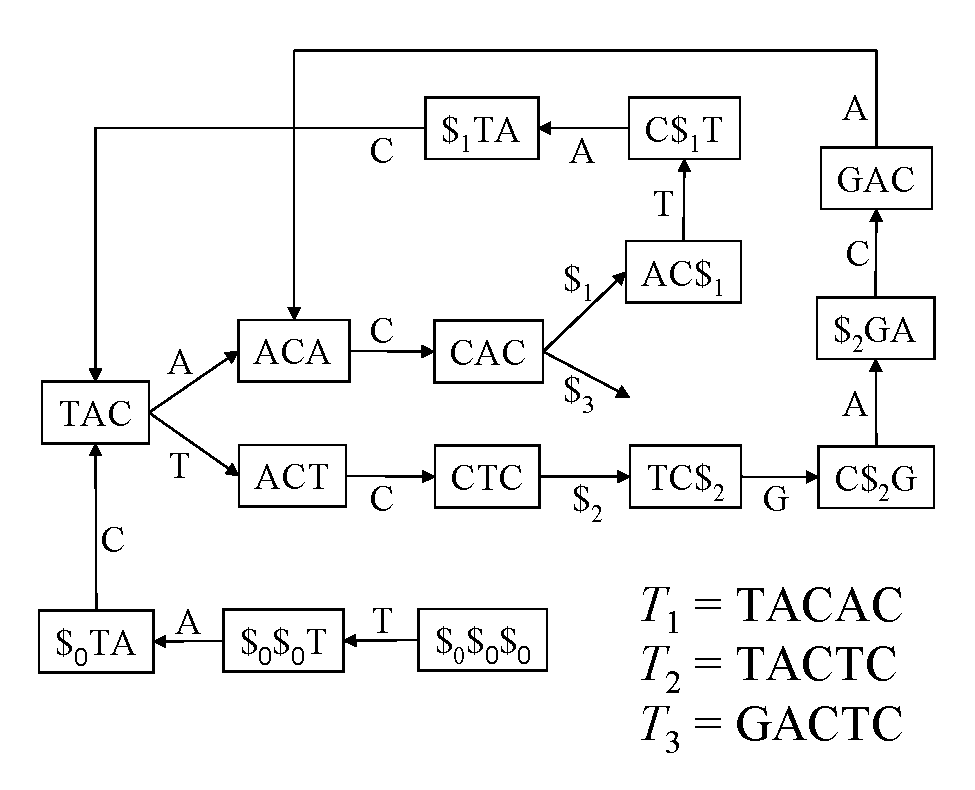
\includegraphics[scale=0.70]{fig3}
\caption{The $3$-dimensional de Bruijn graph of strings `TACAC', `TACTC', and
`GACTC'.}
\label{p1-fig:debruijn}
\end{center}
\end{figure}

\subsection{Basic succinct data structures}\label{p1-sec:rank}

Let $T = T[1] T[2] \cdots T[N]$ be a string of length $N$ on alphabet ${\cal A}$,
that is, $T[i] \in {\cal A}$ for any $i=1,\ldots,N$.
Let $\sigma = |{\cal A}|$ denote the alphabet size.
We can store $T$ in $N \lceil \log_2 \sigma \rceil$ bits.  The space does not
depend on the word size of CPU.  We can retrieve any character $T[i]$ in constant
time using bit operations on words.

The most basic succinct data structure is the one for computing {\rank}, {\select}, and {\access}
values on strings, which are defined as follows.
The value ${\access}(T,i)$ returns $T[i]$ for $1 \le i \le N$.
The value ${\rank}_c(T,i)$ where $c \in {\cal A}$ and $1 \le i \le N$
is the number of $c$'s in $T[1] \cdots T[i]$.  For any $T$ and $c$ we define
${\rank}_c(T,0) = 0$.
The value ${\select}_c(T,j)$ where $c \in {\cal A}$ and $1 \le j \le {\rank}_c(T,N)$
is the position of $j$-th $c$ in $T$.
For any $T$ and $c$ we define ${\select}_c(T,0) = 0$ and for any $j > {\rank}_c(T,N)$
${\select}_c(T,j) = N+1$.
Let $t_r(N,\sigma)$, $t_s(N,\sigma)$, and $t_a(N,\sigma)$ denote the time complexity for computing
{\rank}, {\select}, and {\access}, respectively, on a string of length $N$ and alphabet size $\sigma$.
For brevity, we assume that 
for any $N_1 \le N_2$, $t_r(N_1,\sigma) \le t_r(N_2,\sigma)$ and
for any $\sigma_1 \le \sigma_2$, $t_r(N,\sigma_1) \le t_r(N,\sigma_2)$.
Let $t_b(N,\Sigma)$ denote the maximum of 
$t_r(N,\sigma),t_s(N,\sigma),t_a(N,\sigma)$.

For convenience, we define ${\pred}_c(T,i) = {\select}_c(T, {\rank}_c(T, i))$
which is the position of the first occurrence of $c$ when we scan $T$ from the position $i$ to the head,
and ${\succ}_c(T,i) = {\select}_c(T, {\rank}_c(T, i-1)+1)$
which is the position of the first occurrence of $c$ when we scan $T$ from the position $i$ to the end.
If $T[i]$ is the first (last) occurrence of $c$, {\pred} (\succ) returns $0$ ($N+1$).

%From the definition it holds that
%${\select}_c(T, {\rank}_c(T, i)) \le i$ for any $1 \le i \le n$ and
%${\rank}_c(T, {\select}_c(T, j)) = j$ for any $1 \le j \le {\rank}_c(T,n)$.

There exist many succinct data structures for {\rank} and {\select} on strings.
Among them, we use the one by Ferragina et al.~\cite{FerManMakNav06} for the static case
(the case the string does not change).  A string of $T$ length $n$ on an alphabet of size $\sigma$
can be stored in $nH_0(T) + \Order(\sigma \log n) + \order(n \log\sigma)$ bits so that
{\rank}, {\select} and {\access} queries take $\Order(\log\sigma / \log\log n)$ time,
where $H_0(T)$ denotes the order-$0$ entropy of the string.  Note that if the alphabet size $\sigma$
is $\polylog(n)$, the queries are done in constant time.  For a binary alphabet case,
we can use a simpler data structure that has the same time and space complexities~\cite{RRR07}.

For the dynamic case where the string is modified by inserting or deleting a character,
we use the one by Navarro and Sadakane~\cite{NavSad10} which stores the string
in $nH_0(T) + \Order(\sigma \log n) + \order(n \log\sigma)$ bits so that
{\rank}, {\select} and {\access} queries and insertion and deletion of a character take
$\Order(\frac{\log n}{\log \log n}(1+\frac{\log\sigma}{\log\log n}))$ time.
For polylog-sized alphabets, the operations are done in optimal $\Order(\log n/\log \log n)$ time.
The time complexities for insert and delete are denoted by $t_u(n,\sigma)$.


\subsection{The XBW data structure}
The XBW-transform~\cite{FLMM09} is a method for compressing and indexing labeled trees.
It is an extension of the Burrows-Wheeler transform~\cite{BW94} used for compressing
and indexing strings.  Given a rooted tree with $n$ nodes where each node has a label in
the set of size $\sigma$, the XBW-transform converts the tree into a representation of
$2n + n \log\sigma$ bits.  The size of the representation matches the information-theoretic
lower bound.  We can support tree navigational operations by adding small-size auxiliary
indexes.

Because the XBW is for storing a tree, we cannot use it directly for storing de Bruijn graphs,
which is a cyclic graph.
This paper proposes a new compact representation of de Bruijn graphs of strings.


%%%%%%%%%%%%%%%%%%%%%%%%%%%%%%%%%%%%%%%%%%%%%%%%%%%%%%%%%%%%%%%%%%%%%%%%%%%%%%

\section{Succinct de Bruijn Graphs}\label{p1-sec:sdg}

Let $G$ be a $k$-dimensional de Bruijn graph of a string $T$ of length $N$ on alphabet ${\cal A}$.
Let $n$ and $m$ be the numbers of nodes and edges of $G$, respectively.
A succinct representation of $G$ supports the following operations:
\begin{itemize}
\item ${\cdeg}(v)$ returns the number of outgoing edges from node $v$.
%\item ${\cedge}(v, i)$ 
%\item ${\child}(v, i)$ returns the node $w$ pointed to by the $i$-th outgoing edge of node $v$
%($1 \le i \le {\cdeg}(v)$).
\item ${\child}(v, c)$ returns the node $w$ pointed to by the outgoing edge of node $v$
with edge label $c$.  If no such node exists, it returns $-1$.
\item ${\pdeg}(v)$ returns the number of incoming edges to node $v$.
%\item ${\parent}(v, i)$ returns the node $w$ that is on the $i$-th incoming edge of node $v$
%($1 \le i \le {\pdeg}(v)$).
\item ${\parent}(v, c)$ returns the node $w = (w_1,\ldots,w_k)$ such that 
there is an edge from $w$ and $v$
and $w_1 = c$.  If no such node exists, it returns $-1$.
\item ${\search}(s)$ returns the index $i$ of the node whose label is the string $s$ of length $k$.
%Precisely, $i$ such that ${\last}[i] = 1$ and ${\Node}[i] = s$.
\end{itemize}

We define ${\cal A}^-$ as any set of size $|{\cal A}|$ such that ${\cal A}^- \cap {\cal A} = \emptyset$.
Let $c^-$ denote an element of ${\cal A}^-$ corresponding to an element $c \in {\cal A}$.
We also define a function $u$ as $u(c^-) = c$ for any $c^- \in {\cal A}^-$
and $u(c) = c$ for any $c \in {\cal A}$.  We assume that the function is evaluated in constant time.

\subsection{The succinct representation}

The representation consists of the following components:
\begin{itemize}
\item a string $W = W[1] W[2] \cdots W[m]$ where each character is from ${\cal A} \cup {\cal A}^-$.
\item a string ${\last}$ of length $m$ on the binary alphabet $\{0,1\}$.
\item an array $F$ of length $\sigma = |{\cal A}|$.
\end{itemize}
An example is shown in Figure~\ref{p1-fig:succinctdebruijn}.

The string $W$ is defined as follows.
Each character $W[i]$ represents the label of an edge of $G$.
Each edge $u \rightarrow v$ of $G$ is associated with the node label of $u$.
Those edge labels are sorted in the lexicographic order of reversals of associated node labels.
Ties are broken by edge labels.
Let ${\Node}[i]$ denote the node label for $W[i]$.  This is not explicitly stored.

The string ${\last}$ is defined as
${\last}[i] = 1$ if $i = n$ or ${\Node}[i]$ is different from ${\Node}[i+1]$,
or ${\last}[i] = 0$ otherwise.  From this definition,
all node labels ${\Node}[i]$ with ${\last}[i] = 1$ are distinct, and
those indices $i$ have one-to-one correspondence with the nodes of $G$.
Therefore we use an index $i$ of the strings such that ${\last}[i] = 1$
to represent a node $v$.  
%There are $n$ such indices.
Let $n$ denote the number of nodes.

The array $F$ stores cumulative frequencies of the last characters of node labels.
Namely, for any $c \in {\cal A}$, 
%$F[c] = |\{i \mid 1 \le i \le m, \mbox{the last character of ${\Node}[i]$ is
%smaller than $c$}  \}|$
$F[c] = |\{i \mid 1 \le i \le m, C(i) < c  \}|$
where $C(i)$ denotes the last character of ${\Node}[i]$.
Because $F[\$_i] = i$ for $i = 0,1,\ldots,M$, we need not store them.

The array $F$ is represented in $\Order(\sigma \log m)$ bits.
If $F$ does not change, we can store it as it is using a simple array and $F[c]$ is computed
in constant time.
In a dynamic case that a new node or edge is inserted to the de Bruijn graph,
we have to update $F$ accordingly.  By using a balanced binary tree, $F$ can be maintained
in $\Order(\log \sigma)$ time.

We also use the inverse of $F$, that is, given $i$, we need to know the last character $c$
of ${\Node}[i]$.  In a static case, this can be
computed in constant time using a {\rank}/{\select} data structure of
$\Order(\sigma \log m) + \Order(m \log\log m/\log m)$ bits~\cite{RRR07}.
In a dynamic case, it is done in $\Order(\log \sigma)$ time using a balanced
binary search tree.
%
It can be improved to $\Order(\frac{\log m }{\log \log m}
(1+\frac{\log\sigma}{\log\log m}))$ time using \cite{NavSad10}.
This data structure uses
$\Order(\sigma \log n) + \Order(m \log \log m/\log m)$ bits.
%
Let $t_f$ denote the largest time complexity of those operations.


\begin{figure}[bt]
\begin{center}
  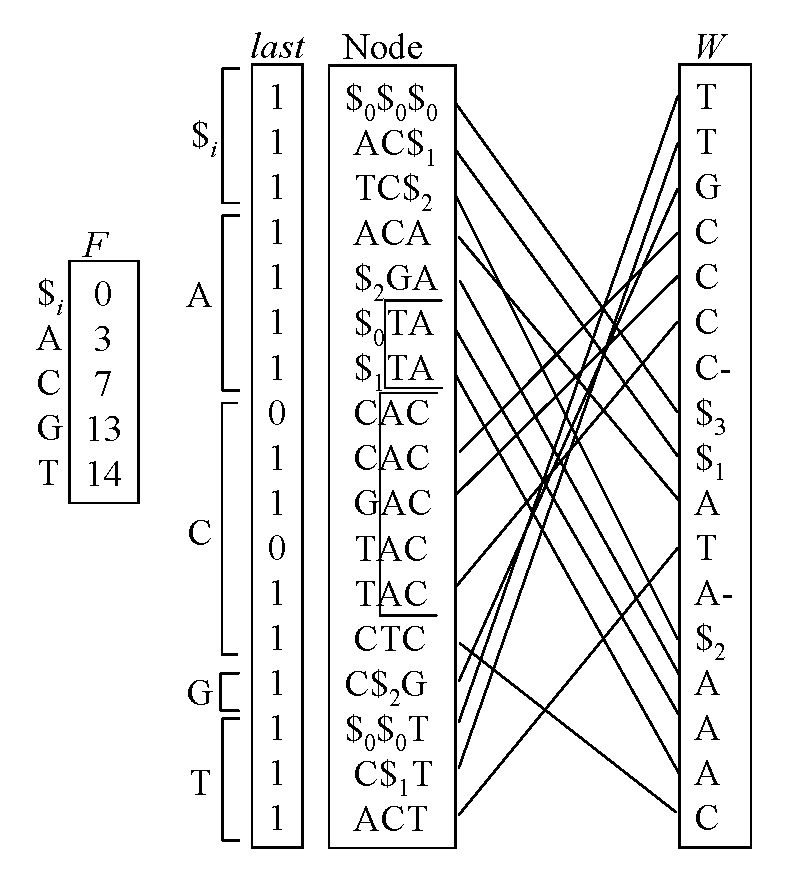
\includegraphics[scale=0.70]{fig4}
\caption{The succinct representation of the de Bruijn graph in Figure~\ref{p1-fig:debruijn}.
Lines between {\Node} and $W$ show {\fwd} and {\bwd} functions.
}
\label{p1-fig:succinctdebruijn}
\end{center}
\end{figure}


A character $W[i]$ is from either ${\cal A}$ or ${\cal A}^-$.
If $W[i]$ is from ${\cal A}^-$, it means that there exists $j < i$ such that
$W[j] = u(W[i])$ and ${\Node}[j]$ and ${\Node}[i]$ have the identical suffix of length $k-1$.

We can define a one-to-one mapping between indices $i$ of ${\last}$ with ${\last}[i] = 1$
and indices $j$ of $W$ with $W[j] \in {\cal A}$.
As stated above, the indices $i$ with ${\last}[i] = 1$ have one-to-one correspondence with
the nodes of the de Bruijn graph $G$.  Consider indices $j$ with $W[j] \in {\cal A}$.
Let ${\Node}^\prime[j]$ denote
the concatenation of the length $k-1$ suffix of ${\Node}[j]$ and $W[j]$.
For any ${\Node}^\prime[j]$, there exists $i$ such that ${\Node}[i] = {\Node}^\prime[j]$.
Because of the definition of $W$, there are no indices $j$ and $j^\prime$ 
($j \neq j^\prime$) such that ${\Node}^\prime[j] = {\Node}^\prime[j^\prime]$.
Therefore there is a one-to-one mapping.  Furthermore, the mapping is represented by
{\rank} and {\select} queries on $W$.
Let $i,j$ be indices such that ${\last}[i] = 1$ and ${\Node}[i] = {\Node}^\prime[j]$.
Let $c = C(i)$ be the last character of ${\Node}[i]$ and 
$r = {\rank}_1({\last}, i) - {\rank}_1({\last}, F[c])$.
Then it holds $j = {\select}_c(W, r)$.  
From $j$, $i$ is computed by $c = W[i]$, $r = {\rank}_c(W, j)$ and
$i = {\select}_1({\last}, {\rank}_1({\last}, F[c]) + r)$.
We define $\bwd(i) = j$ and $\fwd(j) = i$.
The time complexities of $\bwd(i)$ and $\fwd(j)$ are
$\Order(t_f + t_b(m,2\sigma))$.

%Note that the function ${\bwd}(i^\prime)$ for ${\last}[i^\prime] = 0$
%returns the same value as ${\bwd}(i)$ where $i$ is the index such that
%${\last}[i] = 1$ and ${\Node}[i^\prime] = {\Node}[i]$.

Our data structure is similar to the XBW data structure~\cite{FLMM09} in the sense
that the {\last} array in ours is the same as $S_{\last}$ in the XBW.
We propose a new encoding scheme for storing labels of a graph.


\subsection{The {\cdeg} and {\child} operations}
The ${\cdeg}(v)$ operation is easy to support.
We assume that $v$ is the index of ${\last}$ such that ${\last}[v] = 1$ and
${\Node}[v]$ is the label of the node.
From the definition of ${\last}$, it is obvious that 
${\cdeg}(v) = v - {\pred}_1({\last}, v-1)$.
The time complexity is $\Order(t_b(m,2))$.

The ${\child}(v,c)$ operation is done as follows.
For any $1 \le i \le m$, we define $R(i) = [{\pred}_1({\last},i-1)+1,{\succ}_1({\last},i)]$,
which is the range of $W$ and ${\last}$ that for all $j \in R(i)$, ${\Node}[j]$ are identical.
The labels of outgoing edges of node $v$ are stored in $W[j]$ for $j \in R(v)$.
%and they are sorted.  
%
%binary search�����Ȃ��Ă��Crank/select�ł����Ȃ苁�܂��D
%We perform a binary search in the range using the ${\access}$ operation
%on $W$.  Note that during the binary search we regard any character $a^- \in {\cal A}^-$
%as the corresponding character $a$ in ${\cal A}$.
Let $j$ be the index such that $u(W[j]) = c$.
We can find $j$ by ${\pred}_c(W, v)$ and ${\pred}_{c^-}(W, v)$.
Then $x = {\child}(v,c)$ can be computed by $x = \fwd(j)$.

The time complexity for ${\child}(v,c)$ is 
$\Order(t_f + t_b(m, 2\sigma))$.

\subsection{The {\pdeg} and {\parent} operations}
Consider to compute ${\pdeg}(v)$.
Let $d = C(v)$ and $x = bwd(v)$.  Then it holds $d = W[x]$ and the first character
of ${\Node}[x]$ is the label of an edge pointing to $v$.
Let $y = {\succ}_d(W, x)$.  Then all $d^-$ between $W[x]$ and $W[y]$ correspond
to parents of $v$.  The number of such $d^-$ is computed by {\rank} on $W$.
The time complexity is $\Order(t_f + t_b(m,2\sigma))$.

To compute ${\parent}(v,c)$, we need to obtain the first character of ${\Node}[i]$
such that $x \le i < y$ and $u(W[i]) = d$.  The first character of ${\Node}[i]$
is computed by $C(b^{k-1}(i))$ where $b^{k-1}$ stands for applying
${\bwd}({\succ}_1({\last},i))$ repeatedly $k-1$ times.  
We perform a binary search to
find the index $i$ such that $c = C({\bwd}^{k-1}(i))$.
The time complexity is 
$\Order(k(t_f + t_b(m,2\sigma))\log\sigma)$.

\subsection{The {\search} operation}
Recall that ${\search}(s)$ returns the index $i$ of the node whose label 
is the string $s$ of length $k$.
Precisely, it returns $i$ such that ${\last}[i] = 1$ and ${\Node}[i] = s$.
The algorithm for ${\search}(s)$ is similar to \cite{FM05}.
Let $i_1 < i_2 < \cdots < i_w$ be the indices such that
${\last}[i_j] = 1$ and ${\Node}[i_j]$ and $s$ have the same suffix of length $d$ ($1 \le d \le k$).
Let $i_0$ be the smallest index in $R(i_1)$.
Then for any $i$ such that $i_0 \le i \le i_w$, ${\Node}[i]$ and $s$ have the same suffix of length $d$
and for other indices this does not hold.
Therefore ${\search}(s)$ can be done by computing 
ranges $[i_0, i_w]$ for $d = 1,2,\ldots,k$.
Let $c_d$ denote the $d$-th character of $s$ ($1 \le d \le k$).
For $d=1$, the range is $[F[c_1]+1, F[c_1+1]]$.
Given the range $[\ell_d, r_d]$ for $d$,  we can compute the range $[\ell_{d+1}, r_{d+1}]$ for $d+1$
as follows.  The end of the range $r_{d+1}$ is computed by $r_{d+1} = {\child}(r_d, c_{d+1})$.
The beginning of the range $\ell_d$ is computed by ${\pred}_1({\last},{\child}({\succ}_1({\last}, \ell_d), c_{d+1})+1$.

The above algorithm can be simplified.  Instead of computing ranges $[i_0, i_w]$,
we can use $[i_1, i_w]$.  For $d=1$, the range is $[{\succ}_1({\last},F[c_1]+1), F[c_1+1]]$.
Given the range $[\ell_d, r_d]$ for $d$, the range for $d+1$ is obtained by
$r_{d+1} = {\child}(r_d, c_{d+1})$ and $\ell_{d+1} = {\child}(\ell_d, c_{d+1})$.
The time complexity is $\Order(k(t_f + t_b(m,2\sigma)))$.

\subsection{Time and space complexities}
We implement the above data structure for the static case using known succinct data structures.
The array $F$ is stored in $\sigma \log m$ bits.  The data structure for computing $C(i)$
uses $\Order(\sigma \log m) + \Order(m \log \log m/\log m)$ bits.  The operation time $t_f$ is constant.
The string {\last} is stored in $m+\order(m)$ bits so that {\rank}, {\select}, and {\access} takes constant 
time~\cite{RRR07}.  The string $W$ is stored by using \cite{FerManMakNav06}.  
Because the characters
of $W$ are from ${\cal A} \cup {\cal A}^- \cup \{\$_1,\ldots,\$_M\}$, 
the alphabet size is $2\sigma + M$.
%
%Note that there is another character \$ in $W$ which indicates the end of the string, but
%we do not encode it in $W$.  Instead we store the position of the character using $\log m$ bits.
%Then the alphabet size of $W$ is $2\sigma$.  
We can reduce the alphabet size to $2\sigma+1$ by unifying the $M$ terminators
$\$_1,\ldots,\$_M$ into a character \$.  We distinguish two terminators, but
encode them using the same code.

The string $W$ is stored in $m \log (2\sigma+M) +
\Order((\sigma+M) \log m) + \order(m \log\sigma)
 = m + m \log\sigma + \Order((\sigma+M) \log m) + \order(m \log\sigma)$ bits,
and the time complexities $t_r, t_s, t_a$ are 
$\Order(\frac{\log\sigma}{\log\log m})$.
Therefore the time complexities for {\cdeg}, {\pdeg}, {\child}, {\parent},
and {\search} are $\Order(\frac{\log\sigma}{\log\log n})$, 
$\Order(\frac{\log\sigma}{\log\log n})$, 
$\Order(\frac{\log\sigma}{\log\log n})$, 
$\Order(\frac{k\log^2\sigma}{\log\log n})$,
$\Order(\frac{k\log\sigma}{\log\log n})$, respectively.

For polylog-size alphabets, {\cdeg}, {\pdeg} and {\child} takes constant time,
{\parent} takes $\Order(k \log \sigma)$ time,
and {\search} takes $\Order(k)$ time.


%%%%%%%%%%%%%%%%%%%%%%%%%%%%%%%%%%%%%%%%%%%%%%%%%%%%%%%%%%%%%%%%%%%%%%%%%%%%%%

\section{On-line construction}
In this section we propose an on-line construction algorithm of the de Bruijn graph of a string.
Here on-line means given the succinct de Bruijn graph $G$ of a string $T = T[1] \cdots T[N]$, we change it
to the succinct de Bruijn graph $G^\prime$ of the string $T^\prime = T[1] \cdots T[N+1]$ which is made by
appending a character to $T$.
%We give two algorithms; one is space-efficient and the other is faster.
%The former uses no additional space, while the latter uses ..............................
%
%\subsection{Space-efficient algorithm}

As stated above, our succinct representation of $G$ assumes that a character \$ is appended
to the end of $T$.  Let $p$ be the position of \$ in $W$.
To construct the succinct representation of $G^\prime$,
we first change $W[p]$ from \$ to $T[N+1]$ and modify other parts if necessary,
then insert \$ to another position of $W$.  The details are as follows.

Let $p$ be the position of \$ in $W$ for the string $T = T[1] \cdots T[N]$.
If a new character $c = T[N+1]$ is appended to the end of $T$, we change $W[p]$ from \$ to $T[N+1]$.
We have to maintain the invariant that for all $i \in R(p)$, that is, ${\Node}[i] = {\Node}[p]$,
$W[i]$ are distinct.
% and sorted alphabetically.  
%Such $i$'s satisfy
%$p \le i \le {\succ}_1({\last}, p)$.  We do a binary search in this range to find the correct
%position $p^\prime$ for $T[N+1]$.  
Because before changing $W[p]$ they are distinct, we can check the invariant by finding the character
$c = T[N+1]$ or $c^-$ in $W[i]$ such that $i \in R(p)$.  This is done by {\rank} and {\select} on $W$.
%If the same character as $T[N+1]$ does not exist in the range, 
%we insert $T[N+1]$ at the beginning of the range.  Let $x$ denote this position.
%otherwise we do not insert and we delete $W[p]$ and ${\last}[p]$.

If $T[N+1]$ already exists in the range, let $p^\prime$ be its position.
We delete $W[p]$ and ${\last}[p]$ and we insert \$ in $W$ at position $x = {\fwd}(p^\prime)$.
We also insert $0$ in ${\last}[x]$ because ${\Node}[x]$ already exists.
We update $p = x$ and the array $F$ accordingly.

If $T[N+1]$ does not exist in the range,
we change $W[p] = \$ $ to either $c = T[N+1]$ or $c^-$.
To determine $c$ or $c^-$, we first find the nearest occurrence of $c$ to $W[p]$,
namely, its position is $j = {\pred}_c(W, p-1)$ if it exists ($j > 0$).
We compare ${\Node}[j]$ with ${\Node}[p]$.  If they have the same suffix of length $k-1$,
we change $W[p]$ to $c^-$, and otherwise change $W[p]$ to $c$.
We compare characters of ${\Node}[j]$ and ${\Node}[p]$ one by one using the {\bwd} function.
We also compare ${\Node}[j_2]$ with ${\Node}[p]$ where
$j_2 = {\succ}_c(W, p+1)$ if it exists ($j_2 \le m$).
If they share the length $k-1$ suffix, we change $c_2 = W[j_2]$ to $c_2^-$.
This takes $\Order(k(t_f + t_b(m,2\sigma)))$ time.
If the nearest $c$ does not exist ($j = 0$), let $j = F[c]$.
The position $x$ to insert \$ is computed by $x = {\fwd}(j)$.
We insert $0$ to ${\last}[x]$ if $W[p]$ or $W[j_2]$ has a character in ${\cal A}^-$,
or $1$ otherwise.  Finally we set $p = x$ and update the array $F$.

In total, the update operation takes 
$\Order(k(t_f + t_b(m,2\sigma)))$ time.
If we use the dynamic {\rank}/{\select} data structure of \cite{NavSad10}
for $W$ and ${\last}$, $t_b = \Order(\frac{\log m}{\log \log m}(1+\frac{\log\sigma}{\log\log m}))$ time.
We also use \cite{NavSad10} for computing $C(i)$.  Then $t_f = \Order(\frac{\log m }{\log \log m}(1+\frac{\log\sigma}{\log\log m}))$
and the space is $\Order(\sigma \log n) + \Order(m \log \log m/\log m)$ bits.
Because we repeat this update operation $N$ times for all characters of the input string,
the succinct de Bruijn graph can be constructed in
$\Order\left(Nk \cdot \frac{\log m}{\log \log m}
(1+\frac{\log\sigma}{\log\log m})\right)$ time.
For polylog-sized alphabets, it becomes $\Order(Nk \cdot \frac{\log m}{\log \log m})$.

It is easy to construct the static data structure from the dynamic one.
The strings {\last} and $W$ for the static one are generated by
applying {\access} operations to the dynamic one for $i=1,\ldots,m$
in $\Order(m t_b(m,2\sigma))$ time.
After constructing the static strings, the auxiliary data structures for
computing {\rank}/{\select} are constructed in $\Order(m)$ time.

%%%%%%%%%%%%%%%%%%%%%%%%%%%%%%%%%%%%%%%%%%%%%%%%%%%%%%%%%%%%%%%%%%%%%%%%%%%%%%

\section{Conclusion}\label{p1-sec:conclusion}
We have proposed a succinct representation of de Bruijn graphs,
which can be constructed with efficient time and space complexities,
and in an on-line manner.
Therefore they are useful for large-scale genome assembly.

The succinct de Bruijn graph can be also used for data compression.
The PPM (Prediction by Partial Matching) is a text compression algorithm~\cite{CleWit84}.
In the order-$k$ PPM, a character is compressed using statistical information
that it appears after a string of length $k$ based on a given probability distribution.
We can easily extend our succinct de Bruijn graph to be used for PPM compression.
In addition to the array $W$, we use another array to store the numbers of times
that each edge is traversed.  Then we have enough information for compression.
The succinct de Bruijn graph is used for natural language processing because
it stores all $n$-grams in a text.

At the time of publishing, our intended future work was to improve the time complexity for
the on-line construction algorithm, and to implement the data structure and apply it to
assembling large genomes, and PPM data compression. It has since been implemented and used
in the popular assembler MEGAHIT~\cite{megahit}.

The original sample implementation is available at {\tt http://code.google.com/p/csalib/}.


%%%%%%%%%%%%%%%%%%%%%%%%%%%%%%%%%%%%%%%%%%%%%%%%%%%%%%%%%%%%%%%%%%%%%%%%%%%%%%

%\subsection*{Acknowledgments}
%KS and TS are supported in part by KAKENHI 23240002.

%%%%%%%%%%%%%%%%%%%%%%%%%%%%%%%%%%%%%%%%%%%%%%%%%%%%%%%%%%%%%%%%%%%%%%%%%%%%%%
%%%%%%%%%%%%%%%%%%%%%%%%%%%%%%%%%%%%%%%%%%%%%%%%%%%%%%%%%%%%%%%%%%%%%%%%%%%%%%






\chapter{Variable-Order de Bruijn Graphs}

\begin{quote}
%\begin{abstract}
Modern genome sequencing is largely based on a process of randomly breaking replicated copies of a genome into fragments, using various technologies to capture the nucleotide sequence within these fragments (resulting in strings known as reads), and then using assembly software to attempt to reconstruct the original genome sequence from the reads.
This process is challenging as genomes contain repeated regions, and repeated regions much longer than read length confound assemblers, limiting their ability to completely and correctly reconstruct genomes successfully.
Correct and complete genome assembly is important because genomes encode elements that cooperate with others in close proximity, and thus not just the content, but  genome structure has important biological implications.
To the extent quality automated genome reconstruction is possible, there is an additional challenge of accessibility, as some of the most successful assembly software requires unusually high-end servers or clusters.
This limits their usefulness to biologists with access and skill to use such machines and hence more efficient computational techniques are of value.
Beyond efficiency and correctness of algorithms, there is interplay between computational approach, sequencing technology (which vary in read length, accuracy, applicability, and level of detail), and the assembly quality that may result.
In this report, we will expand on the concepts introduced here and review a selection of modern computational assembly tools, the sequence data on which they operate, and discuss important advantages, limitations, and possible extensions of them as well as their relationship to each other in the context of the sequence assembly problem.
%\end{abstract}

\end{quote}
\chapter{Introduction}
\label{chp:introduction}

While consumer-grade genotyping - such as that used by 23andMe - has proven a popular and inexpensive method to determine Single Nucleotide Polymorphisms (SNPs) in individuals, such methods can only detect a set of reference genes, thus limiting their ability to detect all but the simplest variations.

Whole genome sequencing (without a reference) is a powerful alternative, albeit comparatively expensive. However, the price has been steadily declining: while the Human Genome Project cost \$2.7 billion to complete in 2003~\cite{HGP}, as of 2019 it is possible to have a genome sequenced for \$299~\cite{dantelabscost}, and the price continues to drop.

This decline in price is in large part owed to the advent of Next Generation Sequencing (NGS) machines. The “Sanger” sequencing method used in the Human Genome project required a high degree of human interaction, which NGS machines have subsequently automated, greatly increasing the speed and decreasing the cost. And although NGS machines produce much shorter reads (200 bases versus 800 bases in Sanger sequencing - a human genome is 3.4 billion bases), this is overcome by re-sequencing the same DNA.

%There has been another family of DNA sequencers appearing over the past eight years, which can read an entire chromosome at a time. However, they have unpredictable error profiles, making it difficult to sanitize the data, and it is unlikely this will improve without a major breakthrough in physics (cite). Consequently, instead of replacing NGS machines, they are often used in tandem by providing a reference when combining the short read data that NGS machines produce (cite).

The process of combining short reads into longer sequences is called assembly, and while finding the best overlap is NP-hard~\cite{Mye95}, many practical approaches have been proposed (see surveys \cite{KasMor06, MilKor10, Pop09}).

Traditionally, assembly employed an overlap graph, where each read is a node, and an edge exists if two reads have sufficient overlap~\cite{BatJaf02,HuaYan05,MyeSut00}. Assembly then involves computing a Hamiltonian tour of all nodes. This was an acceptable drawback when dealing with Sanger reads, but is prohibitively expensive when dealing with the abundant data that NGS machines produce.

Eulerian assembly~\cite{IW95, PTW} replaces the overlap graph with a de Bruijn graph, where every k-length substring of the reads is a node, and edges represent the k-1 length overlaps, where k is a user selected parameter. The contigs are then found by finding non-branching paths through this graph. Most modern assembler programs use this paradigm~\cite{bankevich2012spades,peng2010idba,Li:2010,Simpson:2009,Butler:2008,Zerbino:2008,SahShi12,MacPrz09}. See \cite{compeau11} for a thorough explanation of de Bruijn graphs and their use in assembly.

\includegraphics*[width=100ex]{images/graph-nodummies.pdf}
\includegraphics*[width=100ex]{images/cdbg.pdf}

While the de Bruijn graph can be constructed more efficiently than the overlap graph, it remains a bottleneck in assembly, both in terms of speed and size, with a de Bruijn graph of a human genome requiring 300 GB of RAM~\cite{Simpson:2009}. Previous work has reduced this to 30 GB~\cite{Conway}. This thesis reduces this to 2 GB, bringing it in line with commodity hardware - a student or field biologist could now perform this on their laptop. Around the same time as the work done in this thesis, an alternative approach with similar performance was published~\cite{wabi}, but the Burrows-Wheeler approach taken in this thesis offers more flexibility and faster edge traversal.

However, it is common for modern assemblers to build multiple de Bruijn graphs. This is because the k parameter significantly influences the topology - if k is too large, the vertices may not have edges, but if k is too small, the graph can become tangled (diagram). The perfect value of k is different for every set of reads, and in fact, due to non-uniform coverage of NGS data, different areas of the same graph may benefit from differing k values. Hence it has become common practice to build multiple graphs with increasing k, and use them in tandem (cite iterative dbg paper). The work in this thesis bypasses this iterative step, and introduces the first de Bruijn graph that can be built once, yet change k values on-the-fly, at only a modest increase in size over the base succinct de Bruijn graph (mention numbers).

Finally, in population genomics, biologists assemble multiple genomes in order to study the variations (give examples and cite). To avoid constructing multiple graphs, Iqbal et al. proposed the Colored de Bruijn Graph~\cite{ICTFM12}. This graph capitalizes on the fact that DNA is rarely unique to an individual. It does this by first constructing a de Bruijn Graph of the entire populations NGS reads, then, each individual is assigned a unique “color”, and the vertices and edges are annotated with the colors that they belong to. In this thesis, we further augment our succinct de Bruijn Graph to efficiently store these colors. When tested with four plant genomes, Iqbal’s structure required 101 GB RAM, while ours only requires 4 GB of RAM. Furthermore, our structure was able to store all known E. Coli genomes in 42 GB, where Iqbal’s was not able to complete, but is estimated to require 3 TB of RAM. We also demonstrate the use of our structure in creating a database of all Antimicrobial Resistance Genes, requiring 245 GB of RAM (an estimated 18 TB with Iqbal’s structure), for rapidly locating resilient bacterial outbreaks in food supply chains.

These three papers demonstrate that the burrows-wheeler approach is efficient, but can also be augmented to support extra queries that are commonplace in many modern assemblers. Due to the wealth of research on Burrows-Wheeler transforms and Suffix Arrays on which the data
structures in this thesis are based, it is likely that the set of supported operations will continue to grow as applications are found.

\section*{Original Work}
%Sections of this thesis are repeated verbatim from these original published papers:
%<each paper title, where it appeared, and a brief description>.
%Succinct de Bruijn Graphs:
%Variable Order de Bruijn Graphs:
%Succinct Colored de Bruijn Graphs:
%

\section{Preliminaries} \label{sec:preliminaries}

%DO WE WANT A FORMAL DEFINITION OF THE DEBRUIJN GRAPH IN HERE?
\subsection{De Bruijn Graphs} \label{sec:dbg}

Given an alphabet $\Sigma$ of $\sigma$ symbols and a set of strings $\lbrace
S_1, S_2, \ldots, S_t \rbrace$, $S_i \in \Sigma^{+}$, the {\em de Bruijn graph}
of order $K$, denoted $G^S_K$, or just $G_K$, when the context is clear, is a
directed, labelled graph defined as follows.

Let $M_{K}$ be the set of distinct $K$-mers (strings of length $K$) that occur
as substrings of some $S_i$. $M_{K+1}$ is defined similarly.  $G_K$ has exactly
$|M_{K}|$ nodes and with each node $u$ we associate a distinct $K$-mer from
$M_{K}$, denoted $\nodelabel(u)$. Edges are defined by $M_{K+1}$: for each
string $T \in M_{K+1}$ there is a directed edge, labelled with symbol $T[K+1]$,
from node $u$ to node $v$, where $\nodelabel(u) = T[1,K]$ and $\nodelabel(v) =
T[2,K+1]$. 

\subsection{Rank and Select} \label{sec:rank} Two basic operations used in almost
every succinct and compressed data structure are {\em rank} and {\em select}.
Given a sequence (string) $S[1,n]$ over an alphabet $\Sigma =
\{1,\ldots,\sigma\}$, a character $c \in \Sigma $, and integers $i$,$j$,
$\rank_c(S,i)$ is the number of times that $c$ appears in $S[1,i]$, and
$\select_c(S,j)$ is the position of the $j$-th occurrence of $c$ in $S$.
%There is a great variety of techniques to answer these queries, with
%suitability depending on the nature of the sequence, for example, on whether or
%not it will be compressed and on the size of the alphabet.
For a binary string $B[1,n]$, the classic solution for rank and
select~\cite{Mun96} is built upon the input sequence, requiring $o(n)$
additional bits.  Generally, $\rank_1$ and $\select_1$ are considered the
default rank and select queries.  More advanced solutions
(e.g.~\cite{bitvector}) achieve zero-order compression of $B$,
%For example, the several structures (e.g.~\cite{bitvector}), (see
%also~\cite{kkp2014}), 
representing it in just $nH_0(B) + o(n)$ bits of space, and supporting $\rank$
and $\select$ operations in constant time. 
%Several practical implementations and improvements of RRR exists (see,
%e.g.,~\cite{kkp2014}).

\subsection{Wavelet Trees} \label{sec:WVT} To support rank and select on larger
alphabet strings, the wavelet tree~\cite{ggv2003,n2013} is a commonly used data
structure that occupies $n\log\sigma + o(n\log\sigma)$ bits of space and
supports $\rank$ and $\select$ queries in $\Oh{\log\sigma}$ time.  Wavelet trees
also support a variety of more complex queries on the underlying string (see,
e.g.~\cite{gnp2012}), in $\Oh{\log\sigma}$ time, and we will make use of some of
this functionality in Section~\ref{sec:implementing}.
%One we will make use of in this paper is the {\em range successor query},
%$\rsucc_c(i,j)$, which returns the smallest character $d > c$ in $S[i,j]$, or
%$\inf$ if no such character exists.  Wavelet trees support \rsucc queries in
%$\Oh{\log\sigma}$ time.


%We will also make use of the Wavelet Tree~\cite{GGV03} data structure on a
%string $T=a_{1}a_{2} \ldots a_{n}$ over an alphabet $\Sigma$.
%
%The Wavelet Tree of $T$ is a binary balanced tree, where each leaf represents a
%symbol of $\Sigma$. The root is associated with the complete sequence $T$. Its
%left child is associated with a subsequence obtained by concatenating the
%symbols $a_i$ of $T$ satisfying $a_i < \sigma /2$. The right child corresponds
%to the concatenation of every symbol $a_i$ satisfying $a_i \geq \sigma$.  This
%relation is maintained recursively up to the leaves, which will be associated
%with the repetitions of a unique symbol.  At each node we store only a binary
%sequence of the same length of the corresponding sequence, using at each
%position a $0$ to indicate that the corresponding symbol is mapped to the left
%child, and a $1$ to indicate the symbol is mapped to the right child.
%
%If the bitmaps of the nodes support constant-time {\em rank} and {\em select}
%queries, then the Wavelet Tree support fast $access$, {\em rank} and {\em
%select} on $T$.
%
%\emph{Access:} In order to obtain the value of $a_{i}$ the algorithm begins at
%the root, and depending on the value of the root bitmap $B$ at position $i$, it
%moves down to the left or to the right child. If the bitmap value is $0$ it
%goes to the left, and replaces $i \leftarrow \rank_{0}(B,i)$. If the bitmap
%value is $1$ it goes to the right child and replaces $i \leftarrow
%\rank_{1}(B,i)$.  When a leaf is reached, the symbol associated with that leaf
%is the value of $a_i$.
%
%\emph{Rank:} To obtain the value of $\rank_c(S,i)$ the algorithm is similar: it
%begins at the root, and goes down updating $i$ as in the previous query, but
%the path is chosen according to the bits of $c$ instead of looking at $B[i]$.
%When a leaf is reached, the $i$ value is the answer.
%
%\emph{Select:} The value of $\select_c(S,j)$ is computed as follows: The
%algorithm begins in the leaf corresponding to the character $c$, and then moves
%upwards until reaching the root.  When it moves from a node to its parent, $j$
%is updated as $j \leftarrow \select_{0}(B,j)$ if the node is a left child, and
%$j \leftarrow \select_{1}(B,j)$ otherwise. When the root is reached, the final
%$j$ value is the answer.
%
%{\em Range Successor Queries}.



\section{BOSS representation}
\label{sec:BOSS}

% TODO: take the concise description of BOSS from CDBG paper?

Conceptually, to build the BOSS representation~\cite{bowe} of a $K$th-order de Bruijn graph from a set of \((K + 1)\)-mers, we first add enough dummy \((K + 1)\)-mers starting with \$s so that if \(\alpha a\) is in the set, then some \((K + 1)\)-mer ends with $\alpha$ ($\alpha$ a $K$-mer, $a$ a symbol).  We also add enough dummy \((K + 1)\)-mers ending with \$ that if \(b \alpha\) is in the set, with $\alpha$ containing no \$ symbols, then some \((K + 1)\)-mer starts with $\alpha$.  We then sort the set of \((K + 1)\)-mers into the right-to-left lexicographic order of their first $K$ symbols (with ties broken by the last symbol) to obtain a matrix.  If the $i$th through $j$th \((K + 1)\)-mers start with $\alpha$, then we say node \([i, j]\) in the graph has label $\alpha$, with \(j - i + 1\) outgoing edges labelled with the last symbols of the $i$th through $j$th \((K + 1)\)-mers.  If there are $n$ nodes in the graph, then there are at most \(\sigma n\) rows in the matrix, i.e., \((K + 1)\)-mers.

For example, if \(K = 3\) and the matrix is the one from Bowe et al.'s paper,
shown in the left of Fig.~\ref{fig:matrix}, then the \(n = 11\) nodes are
\begin{gather*}
 [1, 1], [2, 2], [3, 3], [4, 5], [6, 6], [7, 7], [8, 9], [10,
 10], [11, 11], \\ [12, 12], [13, 13]
\end{gather*}
with labels

\begin{gather*}
 \mathrm{\$\$\$}, \mathrm{CGA}, \mathrm{\$TA}, \mathrm{GAC}, \mathrm{TAC},
\mathrm{GTC}, \mathrm{ACG}, \mathrm{TCG}, \mathrm{\$\$T}, \\
\mathrm{ACT}, \mathrm{CGT},
\end{gather*}%
respectively. The 3rd-order de Bruijn graph itself is shown in the right of the figure.

\begin{figure*}[!t]
\centering
\begin{tabular}{c@{\hspace{10ex}}c}
\begin{tabular}{r@{\hspace{1ex}}@{\hspace{1ex}}@{\hspace{1ex}}l@{\hspace{1ex}}c}
1) & \,\$\,\$\,\$\, & T\\
2) & CGA & C\\
3) & \,\$\,TA & C\\
4) & GAC & G\\
5) & GAC & T\\
6) & TAC & G\\
7) & GTC & G\\
8) & ACG & A\\
9) & ACG & T\\
10) & TCG & A\\
11) & \,\$\,\$\,T & A\\
12) & ACT & \$\\
13) & CGT & C
\end{tabular} &
\raisebox{-10ex}
{\includegraphics*[trim = 0cm 0cm 9cm 24cm, width=50ex]{images/dbg-with-dummies.pdf}}
\end{tabular}
\caption{The BOSS matrix (left) and de Bruijn graph (right) for the quadruples CGAC, GACG, GACT, TACG, GTCG, ACGA, ACGT, TCGA, CGTC.}
\label{fig:matrix}
\hrulefill
\end{figure*}

Bowe et al.\ described a number of queries on the graph, all of which can be implemented in terms of the following three with at most an $\Oh{\sigma}$-factor slowdown:
\begin{itemize}
\item $\forward(v, a)$ returns the node $w$ reached from $v$ by an edge labelled $a$, or NULL if there is no such node;
\item $\backward(v)$ lists the nodes $u$ with an edge from $u$ to $v$;
\item $\lastchar(v)$ returns the last character of $v$'s label.
\end{itemize}
In our example, \(\forward \allowbreak ([8, 9], \mathrm{A}) \allowbreak =
\allowbreak [2, 2]\),
\(\backward \allowbreak ([2, 2]) \allowbreak = \allowbreak [8, 9], [10, 10]\) and
\(\lastchar \allowbreak ([8, 9]) \allowbreak = \allowbreak \mathrm{G}\).
Since $\backward$ always returns at least one node, we can recover any non-dummy node's entire label by $K$ calls to $\lastchar$ interleaved with \(K - 1\) calls to $\backward$.




\section{Varying order}
\label{sec:changing}

If we delete the first column of the matrix in Figure~\ref{fig:matrix}, the result is {\em almost} the BOSS matrix for a 2nd-order de Bruijn graph whose nodes
\[[1, 1], [2, 2], [3, 3], [4, 6], [7, 7], [8, 10], [11, 11], [12, 12], [13, 13]\]
have labels
\[\mathrm{\$\$, GA, TA, AC, TC, CG, \$T, CT, GT}\,,\]
respectively.  Similarly, if we delete the first two columns of the original matrix, the result is almost the BOSS matrix for a 1st-order graph whose nodes
\[[1, 1], [2, 3], [4, 7], [8, 10], [11, 13]\]
have labels
\[\mathrm{\$, A, C, G, T}\,,\]
respectively.  If we delete the first three columns, the result is almost the BOSS graph for the 0th-order graph whose single node \([1, 13]\) has an empty label.  Notice we allow the same node to appear in different graphs, with labels of different lengths.  If readers find this confusing, they can imagine that nodes are triples instead of pairs, with the additional component storing the label's length.

The truncated form of a higher order BOSS differs from the BOSS of a lower order in that
%The problem is that 
some rows are repeated, which could prevent the BOSS representation from working properly.  Suppose that, instead of trying to apply $\forward$, $\backward$ and $\lastchar$ directly to nodes in the new graphs, we augment the BOSS representation of the original graph to support the following three queries:
\begin{itemize}
\item $\shorter(v, k)$ returns the node whose label is the last $k$ characters of $v$'s label;
\item $\longer(v, k)$ lists nodes whose labels have length \(k \leq K\) and end with $v$'s label;
\item $\maxlen(v, a)$ returns some node in the original graph whose label ends with $v$'s label, and that has an outgoing edge labelled $a$, or NULL otherwise. %if there is no such node.
\end{itemize}
If we want a node in the original graph whose label ends with $v$'s label but we do not care about its outgoing edges, then we write \(\maxlen(v, *)\).  Notice $\shorter$ and $\longer$ are symmetric, in the sense that if $v$'s label has length $k_v$ and \(x \in \longer(v, k_v)\), then \(\shorter(x, k_v) = v\).  In our example, \(\shorter([4, 5], 2) = [4, 6]\) while \(\longer([4, 6], 3) = [4, 5], [6, 6]\) and \(\maxlen ([4, 6], \mathrm{G})\) could return either \([4, 5]\) or \([6, 6]\), while \(\maxlen([4, 6], \mathrm{T}) = [4, 5]\) and \(\maxlen([4, 6], \mathrm{A}) = \mathrm{NULL}\).

If $v$ is a node in the original graph --- e.g., $v$ is returned by $\maxlen$ --- then we can use the BOSS implementations of $\forward$, $\backward$ and $\lastchar$.  Otherwise, if $v$'s label has length $k_v$ then
\begin{eqnarray*}
\forward(v, a) & = & \shorter(\forward(\maxlen(v, a), a), k_v)\\
\lastchar(v) & = & \lastchar(\maxlen(v, *))\,.
\end{eqnarray*}
Assuming queries can be applied to lists of nodes, we can compute \(\backward(v)\) as %by computing
\[\shorter(\backward(\maxlen(\longer(v, k_v + 1), *)), k_v),\]
removing any duplicates.

To see why we can compute $\backward$ like this, suppose $v$'s label is \(\alpha a\), so \(\longer(v, \allowbreak k_v + 1)\) returns a list of all \(d \leq \sigma\) nodes whose labels have the form \(b \alpha a\).  Applying $\maxlen$ to this list returns a second list of $d$ nodes, with labels \(\beta_1 b_1 \alpha a, \ldots, \beta_d b_d \alpha a\) of length $K$.  Applying $\backward$ to this second list returns yet a third list, of all the at most \(\sigma d\) nodes whose labels have the form \(c \beta_i b_i \alpha\).  We need only one node returned calling $\backward$ on each node in the second list, so we can discard all but at most $d$ nodes in the third list.  Finally, applying $\shorter$ to the third list returns a fourth list, of all $d$ nodes whose labels have the form \(b_i \alpha\), each of which may be repeated at most $\sigma$ times in the list.



\section{Implementing $\shorter$, $\longer$ and $\maxlen$}
\label{sec:implementing}

The BOSS representation includes a wavelet tree over the last column $W$ of the BOSS matrix, and a bitvector $L$ of the same length with 1s marking where nodes' intervals end.  In our example, \(W = \mathrm{TCCGTGGATAA\$C}\) and \(L = 1110111011111\).

%With these data structures, 
Now we can implement \(\maxlen([i, j], a)\) in $\Oh{\log \sigma}$ time: we use $\rank$ and $\select$ on $W$ to find an occurrence \(W [r]\) of $a$ in \(W [i..j]\), if there is one; we then use $\rank$ and $\select$ on $L$ to find the last bit \(L [i' - 1] = 1\) with \(i' \leq r\) and the first bit \(L [j'] = 1\) with \(j' \geq r\), and return \([i', j']\).  (If there is no occurrence of 1 strictly before \(L [r]\), then we set \(i' = 1\).)  We can implement \(\maxlen([i, j], *)\) in $\Oh{1}$ time: instead of using $\rank$ and $\select$ on $W$ to find $r$, we simply choose any $r$ between $i$ and $j$.

In our example, for \(\maxlen([4, 6], \mathrm{G})\) we first find an occurence \(W [r]\) of G in \(W [4..6]\), which could be either \(W [4]\) or \(W [6]\); if we choose \(r = 4\) then the last bit \(L [i' - 1] = 1\) with \(i' \leq r\) is \(L [3]\) and the first bit \(L [j'] = 1\) with \(j' \geq r\) is \(L [5]\), so we return \([i', j'] = [4, 5]\); if we choose \(r = 6\) then the last bit \(L [i' - 1] = 1\) with \(i' \leq r\) is \(L [5]\) and the first bit \(L [j'] = 1\) with \(j' \geq r\) is \(L [6]\), so we return \([i', j'] = [6, 6]\).

To implement $\shorter$ and $\longer$, we store a wavelet tree over the sequence $L^*$ in which \(L^* [i]\) is the length of the longest common suffix of the label of the node in the original graph whose interval includes $i$, and the label of the node whose interval includes \(i + 1\); this takes $\Oh{\log K}$ bits per \((K + 1)\)-mer in the matrix.  To save space, we can omit $K$s in $L^*$, since they correspond to 0s in $L$ and indicate that $i$ and \(i + 1\) are in the interval of the same node in the original graph; the wavelet tree then takes $\Oh{\log K}$ bits per node in the original graph and $\Oh{n \log K}$ bits in total.  In our example, \(L^* = 0, 1, 0, 3, 2, 1, 0, 3, 2, 0, 1, 1\) (and we can omit the 3s to save space).

For \(\shorter([i, j], k)\), we use the wavelet tree over $L^*$ to find the largest \(i' \leq i\) and the smallest \(j' \geq j\) with \(L^* [i' - 1], L^* [j'] < k\) and return \([i', j']\), which takes $\Oh{\log K}$ time.  For \(\longer([i, j], k)\), we use the wavelet tree to find the set \(B = \{b\,:\,L^* [b] < k\,;\,i - 1 \leq b \leq j\}\) --- which includes \(i - 1\) and $j$ --- and then, for each consecutive pair \((b, b')\) in $B$, we report \([b + 1, b']\); this takes a total of $\Oh{|B| \log K}$ time.  With these implementations, if the time bounds for \(\forward(v, a)\), \(\backward(v)\) and \(\lastchar(v)\) are $\Oh{t_\forward}$, $\Oh{t_\backward}$ and $\Oh{t_\lastchar}$ when $v$ is a node in the original graph, respectively, then they are $\Oh{t_\forward + \log \sigma + \log K}$, $\Oh{\sigma (t_\backward + \log K)}$ and $\Oh{t_\lastchar + 1}$ when $v$ is not a node in the original graph.

In our example, for \(\shorter([4, 5], 2)\) we find the largest \(i' \leq 4\) and the smallest \(j' \geq 5\) with \(L^* [i' - 1], L^* [j'] < 2\) --- which are 4 and 6, respectively --- and return \([4, 6]\).  For \(\longer([4, 6], 3)\) we find the set \(B = \{b\,:\,L^* [b] < 3\,;\,3 \leq b \leq 6\} = \{3, 5, 6\}\) and report \([4, 5]\) and \([6, 6]\).

A smaller but slower approach is not to store $L^*$ explicitly but to support access to any cell \(L^* [i]\) by finding the nodes in the original graph whose intervals include $i$ and \(i + 1\), then using $\backward$ and $\lastchar$ to compute their labels and find the length of their longest common suffix; this takes a total of $\Oh{K (t_\backward + t_\lastchar)}$ time.  To implement $\shorter$ and $\longer$, we store a range-minimum data structure~\cite{fh2011} over $L^*$, which takes \(2 n + o (n)\) bits and returns the position of the minimum value in a specified substring of $L^*$ in $\Oh{1}$ time.

For \(\shorter([i, j], k)\), we use binary search and range-minimum queries to find the largest \(i' \leq i\) and the smallest
\(j' \geq j\) with \(L^* [i' - 1], L^* [j'] < k\) and return \([i', j']\), which takes $\Oh{K (t_\backward + t_\lastchar) \log (n \sigma)}$ time. 
%(With a more complicated use of the range-minimum data structure, which we will describe in the full version of this paper, we use $\Oh{K^2 (t_\backward + t_\lastchar)}$ time.)
For \(\longer([i, j], k)\), we recursively split \([i, j]\) into subintervals with range-minimum queries, at each step using $\backward$ and $\lastchar$ to check that the minimum value found is less than $k$; this takes $\Oh{K (t_\backward + t_\lastchar)}$ time per node returned.  With these implementations, \(\forward(v, a)\), \(\backward(v)\) and \(\lastchar(v)\) take $\Oh{t_\forward + K (t_\backward + t_\lastchar) \log (n \sigma)}$, $\Oh{\sigma K (t_\backward + t_\lastchar) \log (n \sigma) + \sigma^2 t_\backward}$ and $\Oh{t_\lastchar + 1}$ time, respectively, when $v$ is not a node in the original graph.

For \(\sigma = \Oh{1}\), our bounds are summarized in the following theorem. % We will provide more details in the full version of this paper.

\begin{theorem}
\label{thm:bounds}
When \(\sigma = \Oh{1}\), we can store a variable-order de Bruijn graph in $\Oh{n \log K}$ bits on top of the BOSS representation, where $n$
is the number of nodes in the $K$th-order de Bruijn graph, and support \forward\ and \backward\ in $\Oh{\log K}$ time and \lastchar\ in
$\Oh{1}$ time.  We can also use $\Oh{n}$ bits on top of the BOSS representation, at the cost of using $\Oh{K \log n / \log \log n}$ time
for \forward\ and \backward.
\end{theorem}

%shorter - logK
%longer - |B| log K time (for a set of B resulting nodes)

%K^2 log^2 n / log log n

%O(B K^2 log^2 n / log log n)

\section{Experiments}
\label{sec:experiments}

\begin{table}[t!]
%\caption{Construction Time and Memory Usage (top), and Mean Time per Navigation Operation (lower).}
\caption{Input size (top), construction time, memory use, and structure size (middle), and mean time taken for each 
navigation operation (lower), for all data sets and both structures. For variable-order, the multipliers in
parenthesis are the increase over the fixed-order results. Cells marked ``N/A'' for fixed-order indicate operations not
possible with that structure.
%The times in parentheses for $\longer$ are the mean times per node in the resulting set.
}
\scriptsize
\setlength\tabcolsep{1.8pt}
\begin{tabularx}{\textwidth}{@{}Rd{3.2}d{4.9}d{3.2}d{4.9}d{3.2}d{5.9}d{3.2}d{5.9}@{}}
% manual : http://ftp.jaist.ac.jp/pub/CTAN/macros/latex/required/tools/tabularx.pdf
						%\cline{2-9}
\toprule
{\bf Dataset}     & \multicolumn{2}{c}{{\em E.~coli}} & \multicolumn{2}{c}{Human chromosome 14} & \multicolumn{2}{c}{Human} 		& \multicolumn{2}{c}{Parrot} \\
% I think DSK size + number of K-mers is enough to demonstrate the increasing data set size
% I don't have times for DSK, so I'd have to run those again if needed
%Genome Size (bp) & \multicolumn{2}{c}{{4,639,221}} & \multicolumn{2}{c}{88,289,540} & \multicolumn{2}{c}{} 		& \multicolumn{2}{c}{} \\
%Number of Reads & \multicolumn{2}{c}{{}} & \multicolumn{2}{c}{} & \multicolumn{2}{c}{} 		& \multicolumn{2}{c}{} \\
%\midrule
%K & \multicolumn{2}{c}{{27}} & \multicolumn{2}{c}{55} & \multicolumn{2}{c}{55} 		& \multicolumn{2}{c}{55} \\
%Frequency Threshold & \multicolumn{2}{c}{{1}} & \multicolumn{2}{c}{1} & \multicolumn{2}{c}{2} 		& \multicolumn{2}{c}{1} \\
%DSK Time (mins) & \multicolumn{2}{c}{{}} & \multicolumn{2}{c}{} & \multicolumn{2}{c}{} 		& \multicolumn{2}{c}{} \\
{\bf DSK Size (GB)} & \multicolumn{2}{c}{{1.52}} & \multicolumn{2}{c}{6.88} & \multicolumn{2}{c}{26.74} 		& \multicolumn{2}{c}{70.28} \\
{\bf\boldmath Number of $K$-mers} & \multicolumn{2}{c}{{204,098,902}} & \multicolumn{2}{c}{461,445,333} & \multicolumn{2}{c}{1,794,522,954} 		& \multicolumn{2}{c}{4,716,731,435} \\
{\bf BOSS Order} & \multicolumn{1}{c}{fixed} 	& \multicolumn{1}{c}{variable} & \multicolumn{1}{c}{fixed} 	& \multicolumn{1}{c}{variable} & \multicolumn{1}{c}{fixed} 	& \multicolumn{1}{c}{variable} & \multicolumn{1}{c}{fixed} 	& \multicolumn{1}{c}{variable} \\
\midrule
%\cline{1-9}
{\bf Construction (mins)} & 3.93 & 5.09 \enspace (1.30{\sf x}) & 14.37 & 18.72 \enspace (1.30{\sf x}) & 64.45 & 83.85 \enspace (1.30{\sf x})& 162.58 & 225.73 \enspace (1.39{\sf x})\\
{\bf Graph Size (GB)}  			   & 0.16  & 0.41 \enspace (2.56{\sf x})  & 0.40   & 1.38 \enspace (3.45{\sf x}) & 1.67 & 5.42 \enspace (3.25{\sf x}) & 4.20 & 13.60 \enspace (3.24{\sf x}) \\
{\bf Peak RAM (GB)}  		 & 3.16 & 3.16 \enspace (1.00{\sf x}) & 3.22 & 3.22 \enspace (1.00{\sf x})& 7.65 & 9.31 \enspace (1.22{\sf x}) & 15.30 & 15.29 \enspace (1.00{\sf x}) \\
{\bf Peak Disk (GB)}  	 & 12.17 & 12.17 \enspace (1.00{\sf x}) & 56.68 & 56.68 \enspace (1.00{\sf x}) & 248.37 & 248.37 \enspace (1.00{\sf x}) & 562.28 & 562.28 \enspace (1.00{\sf x})\\
%\cline{1-9}
\midrule
$\forward$ ($\mu$s)   & 6.00 & 17.03 \enspace (2.84{\sf x}) &6.24	&16.17 \enspace (2.59{\sf x}) &7.07	&18.31 \enspace (2.59{\sf x})&7.77	 &19.39 \enspace (2.50{\sf x})\\
$\backward$ ($\mu$s)  & 8.23 & 59.77 \enspace (7.26{\sf x}) &8.47	&55.63 \enspace (6.57{\sf x}) &9.27	&62.85 \enspace (6.78{\sf x})&10.46 &63.87 \enspace (6.11{\sf x})\\
$\lastchar$ ($\mu$s)  & 0.01 &  0.01 \enspace (1.00{\sf x}) &0.01	& 0.01 \enspace (1.00{\sf x}) &0.01	& 0.01 \enspace (1.00{\sf x})&0.01	 &0.01 \enspace (1.00{\sf x})\\

$\maxlen$ ($\mu$s)    &\multicolumn{1}{r}{N/A}  & 1.43   &\multicolumn{1}{r}{N/A} &1.56	   &\multicolumn{1}{r}{N/A}  	&2.02	    &\multicolumn{1}{r}{N/A}  &2.46 \\ 
$\maxlen_c$ ($\mu$s)  &\multicolumn{1}{r}{N/A}  &	5.41  &\multicolumn{1}{r}{N/A} &5.98	   &\multicolumn{1}{r}{N/A}  &6.71	    &\multicolumn{1}{r}{N/A}  &7.49 \\
$\shorter_1$ ($\mu$s) &\multicolumn{1}{r}{N/A}   &	14.65 &\multicolumn{1}{r}{N/A} &17.72	 &\multicolumn{1}{r}{N/A} 	  &19.54	  &\multicolumn{1}{r}{N/A}  &19.84 \\
$\shorter_2$ ($\mu$s) &\multicolumn{1}{r}{N/A}  &	14.83 &\multicolumn{1}{r}{N/A} &17.79	 &\multicolumn{1}{r}{N/A}  	&19.68	  &\multicolumn{1}{r}{N/A}  &19.98 \\
$\shorter_4$ ($\mu$s) &\multicolumn{1}{r}{N/A}   &	15.11 &\multicolumn{1}{r}{N/A} &18.02	 &\multicolumn{1}{r}{N/A}   &19.90	  &\multicolumn{1}{r}{N/A}  &20.20 \\
$\shorter_8$ ($\mu$s) &\multicolumn{1}{r}{N/A}   &	15.73 &\multicolumn{1}{r}{N/A} &18.39	 &\multicolumn{1}{r}{N/A}   &20.29	  &\multicolumn{1}{r}{N/A}  &20.64 \\
%$\shorter$ ($\mu$s)   &\multicolumn{1}{r}{N/A}   &	15.08 &\multicolumn{1}{r}{N/A} &17.98	 &\multicolumn{1}{r}{N/A}   &19.85	  &\multicolumn{1}{r}{N/A}  &20.17 \\ % mean avg of above 4
$\longer_1$ ($\mu$s)  &\multicolumn{1}{r}{N/A}   &21.53   &\multicolumn{1}{r}{N/A} &18.61	 &\multicolumn{1}{r}{N/A}   &21.06	  &\multicolumn{1}{r}{N/A}  &20.57 \\ 
$\longer_2$ ($\mu$s)  &\multicolumn{1}{r}{N/A}  &56.96   &\multicolumn{1}{r}{N/A} &41.08	 &\multicolumn{1}{r}{N/A}   &49.01	  &\multicolumn{1}{r}{N/A}  &47.07\\
$\longer_4$ ($\mu$s)  &\multicolumn{1}{r}{N/A}   &503.60  &\multicolumn{1}{r}{N/A} &323.50	 &\multicolumn{1}{r}{N/A}   &446.51	  &\multicolumn{1}{r}{N/A}  &428.97 \\
$\longer_8$ ($\mu$s)  &\multicolumn{1}{r}{N/A}  &6441.33 &\multicolumn{1}{r}{N/A}  &5338.38 &\multicolumn{1}{r}{N/A}   &18349.80	&\multicolumn{1}{r}{N/A}  &24844.80 \\

%$\longer_1$ ($\mu$s)  &\multicolumn{1}{r}{N/A} &21.53 \enspace (10.82)  &\multicolumn{1}{r}{N/A} &18.61 \enspace (12.38)  &\multicolumn{1}{r}{N/A} &21.06 \enspace (13.25)    &\multicolumn{1}{r}{N/A} &20.57 \enspace (12.99)\\ 
%$\longer_2$ ($\mu$s)  &\multicolumn{1}{r}{N/A} &56.96 \enspace (8.74)   &\multicolumn{1}{r}{N/A} &41.08 \enspace (11.24)  &\multicolumn{1}{r}{N/A} &49.01 \enspace (11.74)    &\multicolumn{1}{r}{N/A} &47.07 \enspace (11.02)\\
%$\longer_4$ ($\mu$s)  &\multicolumn{1}{r}{N/A} &503.60 \enspace (7.98)  &\multicolumn{1}{r}{N/A} &323.50 \enspace (10.59) &\multicolumn{1}{r}{N/A} &446.51 \enspace (11.04)   &\multicolumn{1}{r}{N/A} &428.97 \enspace (9.95)\\
%$\longer_8$ ($\mu$s)  &\multicolumn{1}{r}{N/A} &6441.33 \enspace (6.44) &\multicolumn{1}{r}{N/A} &5338.38 \enspace (9.03) &\multicolumn{1}{r}{N/A} &18349.80 \enspace (10.09) &\multicolumn{1}{r}{N/A} &24844.80 \enspace (9.48)\\

%$\longer_1$ nodes&	N/A	39.80	N/A	30.06	N/A	31.78	N/A	31.66
%$\longer_2$ nodes&	N/A	130.32	N/A	73.11	N/A	83.48	N/A	85.42
%$\longer_4$ nodes&	N/A	1262.84	N/A	610.77	N/A	809.06	N/A	861.91
%$\longer_8$ nodes&	N/A	20010.15	N/A	11824.04	N/A	36370.68	N/A	52388.38
\bottomrule
%\cline{2-9}
\end{tabularx}
% $\dagger$ $\lastchar$ is a reverse lookup in a very small array, so the speed is in fractions of a nanosecond.
% $\ddagger$ $\longer$ is reported as the average time  for the inputs $1$,$2$,$4$,$8$, due to much longer calculation time. }
\label{tab:nav-time}
\end{table}

%We have implemented the faster version of our data structure on top of an efficient implementation of the BOSS single-$K$ data structure\footnote{The
We have implemented the wavelet tree based data structure on top of an efficient implementation of the BOSS single-$K$ data structure\footnote{The
implementation is released under GPLv3 license at \url{http://github.com/cosmo-team/cosmo}. As Cosmo is under continuous development,
a static snapshot of the code used in this paper is available at \url{https://github.com/cosmo-team/cosmo/tree/varord-paper}.}.
Both structures make use of the SDSL-lite software library\footnote{\url{https://github.com/simongog/sdsl-lite}} for succinct data structures, and the
the construction code makes use of the STXXL software library\footnote{\url{https://github.com/stxxl/stxxl}} for external memory data structures and sorting.
The construction code is also concurrent in many places.%, making use of C++11 threads, and OpenMP\footnote{\url{http://openmp.org/}} for parallel internal memory sorting.
The smaller but slower version was not implemented.
%Further implementation details are described in \ref{sec:implementation}.

% TODO : cite their algorithmic paper?
% What makes STXXL good:
% http://stxxl.sourceforge.net/tags/master/introduction.html
% http://stxxl.sourceforge.net/tags/master/design.html
% http://stxxl.sourceforge.net/tags/master/design_algo_sorting.html
% http://stxxl.sourceforge.net/tags/master/citelist.html

% System
Our test machine was a server with a hyperthreaded quad-core 2.93 Ghz Intel Core i7-875K CPU and 16 GB RAM running
Ubuntu Server 14.04. Four Samsung 850 EVO 250GB SSDs were used for temporary storage for STXXL,
with a fifth identical drive used for temporary storage for SDSL-Lite and final graph output. In order to make
use of STXXL's parallel disk and asynchronous I/O support\footnote{\url{http://stxxl.sourceforge.net/tags/master/design_algo_sorting.html}},
the SSDs were not in a RAID configuration. The input files were read from a mechanical 2TB 7200 RPM disk.
% I might have been able to load the DSK files from a SSD thinking back... but it wouldn't make a difference except faster run time *for everything*

To minimize the effect of external factors on our results, each experiment was repeated three times with the minimum values
reported. The swap file was disabled, forcing the operating system to keep each graph completely in memory, and
there were no other users on the server.

% TODO : should construction be moved up and merged with the above?
% TODO : describe the construction algorithm
% TODO : describe why we needed external construction

\subsection{Test Data}

%To assess assembly quality, we aligned the reads to the {\em E.~coli} reference genome (substr.  K-12) using BWA (version 0.5.9) \cite{li2009fast} with default parameters.  We call a read {\em mapped} if BWA outputs an alignment for it and {\em unmapped} otherwise.  Analysis of the alignments revealed that 98\% of the reads mapped to the reference genome, representing an average depth of approximately $600\times$.  Next, we determined the amount of memory and time needed for our method for a larger dataset.  For that, we 
%The reference genome was also downloaded from the website (Reference genome GCA\_000001405.16).  
% Analysis of the alignments revealed that 98\% of the reads mapped to the reference genome, which represents 
% approximately 47x coverage of the genome.

In order to test the scalability of our approach, we repeated the experiment on readsets of varying size.
Our first data set consists of 27 million paired-end 100 character reads (strings)
from {\em E.~coli} (substr.  K-12). It was obtained from the NCBI Short Read Archive (accession 
ERA000206, EMBL-EBI Sequence Read Archive). The total size of this data set is around 2.3 GB compressed on disk (6 GB uncompressed).

The second data set is 36 million 155 character reads from the Human chromosome 14 Illumina reads used in the GAGE
benchmark\footnote{\url{http://gage.cbcb.umd.edu/}}, totalling 1.3 GB compressed on disk (6 GB uncompressed).

For our third data set we obtained 1,415 million  paired-end 100 character Human genome reads
(SRX01231) that were generated by Illumina Genome Analyzer (GA) IIx platform. The total size of this data set is 130 GB compressed on disk (470 GB uncompressed).

Our fourth data set is 700 million paired-end 101 character reads, and 131 paired-end 75 character reads from the short
insert libraries of the Parrot data (ERA201590) provided in Assemblathon 2\cite{assemblathon2}.
The total size of this data set is 64 GB compressed on disk (245 GB uncompressed).

%We ran DSK on each... The human data set required too much external memory, and the final dBG size would have been too large to fit in internal memory,
%so had to be re-run with the frequency threshold set to 2.

We used DSK~\cite{dsk} on each data set to find the unique $(K+1)$-mers.
It is usual to have DSK ignore low-frequency $(K+1)$-mers (as they may result from sequencing errors). 
However, removing such $(K+1)$-mers may result in the removal of some $k$-mers with $k \leq K$ that would 
otherwise have an acceptable frequency. We therefore set the frequency threshold to be as low as possible: $1$ (accepting 
all $(K+1)$-mers) for all data sets except for the Human genome data set, which was too big for our SSDs during construction,
and too big to fit into RAM afterwards. Hence, for the Human genome data set, the frequency threshold was $2$.

%\footnote{This increases the resulting size, but the size relative to the standard BOSS representation can still be compared.
%Variable-$K$ frequency filtering can be implemented using the $L^*$ vector, but will affect the dummy edge calculations, and
%is hence designated as future work.}.
% TODO: mention mercy kmers (Megahit) as another strategy? ultimately we just don't want gaps

A value of $K = 27$ was chosen
%\footnote{Note that the BOSS de Bruijn graph is defined in terms of $K+1$-mers, so DSK must be run for $K+1$ (i.e. 28 and 56) rather than for $K$.}
for the {\em E.~coli} data, and $K = 55$
for the Human data sets as these values produced good assemblies in previous papers (see, e.g.,~\cite{paul}). $K = 55$ was also chosen for the Parrot
data set, %as there was no clear choice for $K$ from the Assemblathon 2 contestants, and
as it produced a graph that almost filled the main memory.
The resulting file sizes and $(K+1)$-mer totals are shown in Table~\ref{tab:nav-time}.

% TODO: Run experiment with one data set over multiple Ks to see how it scales that way

% TODO: Time DSK (multithreaded) (I don't have timings for these)
%DSK took 28 and 58 minutes to run on the {\em E.~coli} and human data sets, respectively.

\subsection{Construction}
\label{sec:construction}

In order to convert the input DSK data to the format required by BOSS (in the correct order, with dummy edges, as required by both single-$K$ and variable-$K$ structures),
we use the following process, which has been designed with disk I/O in mind.

While reading the DSK input data, we generate and add the reverse complements for each $(K+1)$-mer, then sort them by their first $K$ symbols (the source nodes). Concurrently, we also sort another copy of the $(K+1)$-mers and their reverse complements by their last $K$ symbols (the target nodes). Let the resulting tables
be $A$ and $B$, respectively.

Next, we calculate the set differences $A-B$, comparing only the $K$-length prefixes to the $K$-length suffixes respectively. This tells us which source nodes do not
appear as target nodes, which we prepend with $\$$ signs to create the required incoming dummy edges ($K$ each), and then sort by the first $K$ symbols. Concurrently, we also calculate $B-A$ to give us
the nodes requiring outgoing dummy edges (to which we append $\$$). Let the resulting tables be $I$ and $O$, respectively. At this point $B$ can be deleted.
%\footnote{This will create duplicate strings, which can be avoided using Longest Common Prefix calculations.}.

Finally, we perform a three-way merge (by first $K$ symbols) of $A$, $I$, and $O$, outputting the rightmost column. In the case of the variable-$K$ graph,
we also calculate the $L^{*}$ values while merging. Finally, we construct the necessary succinct indexes from the output.

The time bottleneck in the above process is clearly in sorting the $A$ and $I$ tables. $|I|$ can be as big as $K|A|$, but in practice only $1\%$ or fewer
nodes require incoming dummies. Our elements are of size $\Oh{K}$, thus, overall, construction of both data structures takes $\Oh{K^2|A|\log|A|}$ time
and $\Oh{K^2|A|}$ space in theory, but in practice takes $\Oh{K|A|\log|A|}$ time and $\Oh{K|A|}$ space.

%The large file sizes necessitated an external construction scheme.

% Draw attention to the limited difference
%The only place that construction differs for the variable order de Bruijn graph is during the merge, where the longest common suffix length is calculated
%for consecutive edges, and written to disk. Finally, when constructing the rank and select structures, the variable order de Bruijn graph creates a Wavelet Tree
%as well.


\subsection{Results}

For each data set, the $(K+1)$-mers from DSK (and their reverse complements) were converted into the BOSS format
using the process outlined in \ref{sec:construction}, using the external memory vectors and multithreaded, external
memory sort from STXXL. The BOSS structure and $L^{*}$ wavelet tree were then built using indexes from SDSL-lite.

Construction times and structure sizes are shown in Table~\ref{tab:nav-time}.
While the variable-$K$ BOSS structure is around $30\%$ slower to build, and $2.6$ to $3.5$ times larger 
than the standard BOSS structure, this is clearly much faster and less space consuming than building 
$K$ separate instances of the BOSS structure. The peak RAM and disk usage is the same for both structures
except in the case of the Human genome data set, where the variable-$K$ BOSS structure used $22\%$ more RAM.
% TODO : repeat, if same results, trace RAM usage, work out why?

% identical peak disk and RAM
% TODO : Does this sounds week since we didn't measure building/storing each static-k dbg individually?
% TODO : Should we compare it to megahit?

%% TODO: fix the xs in this table? \times doesnt handle \em well though
%\begin{table}[h!]
%\begin{tabularx}{\textwidth}{@{\extracolsep{\fill} } r  c  c   c  c }
%						& \multicolumn{2}{c}{{\em Escherichia coli}} 		& \multicolumn{2}{c}{Human chromosome 14} \\
%						\cline{2-5}
%   						& BOSS 		& multi-K BOSS			& BOSS  		&  multi-K BOSS  \\
%\hline
%Wall Time (mins) & 19  & 25 {\em(1.32x)} & 153 & 203 {\em(1.33x)} \\
%Final Size (MB)  & 163 & 420 {\em(2.58x)} & 414 & 1416 {\em(3.42x)}\\
%Genome Size (bp) 	&  \multicolumn{2}{c}{4,639,221} 			&  \multicolumn{2}{c}{88,289,540} \\
%Number of Reads 			&  \multicolumn{2}{c}{27 M} 				&  \multicolumn{2}{c}{36.5 M}  \\
%DSK Time (mins) 	&  \multicolumn{2}{c}{28} 			&  \multicolumn{2}{c}{58} \\
%\hline
%\end{tabularx}
%\caption{Summary of data sets, as well as construction time and final space for BOSS de Bruijn graph and multi-$K$ de Bruijn graph. For the multi-$K$ BOSS representation, the
%increase factor is shown in parentheses.}
%\label{tab:build}
%\end{table}

%Due to the non-trivial engineering effort required to integrate a particular de Bruijn graph 
%structure in a live assembler, we compare our new data structure to the original BOSS structure
%by measuring average times for navigation operations.
To measure navigation functions $\forward$ and $\backward$ we took the mean time 
over 20,000 random queries. For the variable-$K$ graph, the $k$ values for each node 
were chosen randomly between $8$ and $K$. 
%(involves only a reverse lookup on a very small array). 
Results are shown in Table~\ref{tab:nav-time}. 
The new structure makes the $\forward$ operation $2.5$ to $3$ times slower for $k < K$, though we 
note that for $k = K$ $\forward$ time is identical.
The $\backward$ operation is much slower in the new structure, but is much less frequently 
used than $\forward$ in assembly algorithms (for a variation that supports fast
$\backward$ calculations, see \cite{varorder-latin}). We also measured $\lastchar$, which took only
nanoseconds on both structures.

To see how fast the order can be changed, we timed $\shorter$ and $\longer$ for
changes of $1$, $2$, $4$, and $8$ symbols. Our experiments show that in practice changing 
order by a single symbol ($\shorter_1$ and $\longer_1$) is a cheap operation, taking around the
same time as $\forward$. For larger changes in order, the time for $\shorter$ is stable
($\shorter_1$, $\shorter_2$, $\shorter_4$, and $\shorter_8$ all take roughly the same time),
whereas $\longer$ takes significantly more time as the difference in order increases. This is because
$\longer$ must compute a set of nodes, and the size of that set grows roughly exponentially with
the change in order ($\longer$ takes around $10 \mu$s per node when averaged over the size of the resulting set).
%If not every node in the result is to be visited, the set could instead be calculated lazily.

As expected, $\maxlen$ is very fast (it requires a single rank and select operation
over a bit vector), and only slightly affected when finding the specified outgoing edge label (which
uses a rank and select over the BOSS wavelet tree instead).

% TODO: add separate measurements for 2,4,8... but as order changes increase, the... factor is more evident.



\chapter{Conclusions}
\label{sec:conclusions}

%\section{Future Work}
%\label{sec:future-work}


%\subsection*{Acknowledgments}
%We thank two anonymous reviewers for thoughtful comments that materially improved this manuscript.
%
\chapter{Succinct Colored de Bruijn Graphs}

\begin{quote}
%\begin{abstract}
Modern genome sequencing is largely based on a process of randomly breaking replicated copies of a genome into fragments, using various technologies to capture the nucleotide sequence within these fragments (resulting in strings known as reads), and then using assembly software to attempt to reconstruct the original genome sequence from the reads.
This process is challenging as genomes contain repeated regions, and repeated regions much longer than read length confound assemblers, limiting their ability to completely and correctly reconstruct genomes successfully.
Correct and complete genome assembly is important because genomes encode elements that cooperate with others in close proximity, and thus not just the content, but  genome structure has important biological implications.
To the extent quality automated genome reconstruction is possible, there is an additional challenge of accessibility, as some of the most successful assembly software requires unusually high-end servers or clusters.
This limits their usefulness to biologists with access and skill to use such machines and hence more efficient computational techniques are of value.
Beyond efficiency and correctness of algorithms, there is interplay between computational approach, sequencing technology (which vary in read length, accuracy, applicability, and level of detail), and the assembly quality that may result.
In this report, we will expand on the concepts introduced here and review a selection of modern computational assembly tools, the sequence data on which they operate, and discuss important advantages, limitations, and possible extensions of them as well as their relationship to each other in the context of the sequence assembly problem.
%\end{abstract}

\end{quote}
\chapter{Introduction}
\label{chp:introduction}

While consumer-grade genotyping - such as that used by 23andMe - has proven a popular and inexpensive method to determine Single Nucleotide Polymorphisms (SNPs) in individuals, such methods can only detect a set of reference genes, thus limiting their ability to detect all but the simplest variations.

Whole genome sequencing (without a reference) is a powerful alternative, albeit comparatively expensive. However, the price has been steadily declining: while the Human Genome Project cost \$2.7 billion to complete in 2003~\cite{HGP}, as of 2019 it is possible to have a genome sequenced for \$299~\cite{dantelabscost}, and the price continues to drop.

This decline in price is in large part owed to the advent of Next Generation Sequencing (NGS) machines. The “Sanger” sequencing method used in the Human Genome project required a high degree of human interaction, which NGS machines have subsequently automated, greatly increasing the speed and decreasing the cost. And although NGS machines produce much shorter reads (200 bases versus 800 bases in Sanger sequencing - a human genome is 3.4 billion bases), this is overcome by re-sequencing the same DNA.

%There has been another family of DNA sequencers appearing over the past eight years, which can read an entire chromosome at a time. However, they have unpredictable error profiles, making it difficult to sanitize the data, and it is unlikely this will improve without a major breakthrough in physics (cite). Consequently, instead of replacing NGS machines, they are often used in tandem by providing a reference when combining the short read data that NGS machines produce (cite).

The process of combining short reads into longer sequences is called assembly, and while finding the best overlap is NP-hard~\cite{Mye95}, many practical approaches have been proposed (see surveys \cite{KasMor06, MilKor10, Pop09}).

Traditionally, assembly employed an overlap graph, where each read is a node, and an edge exists if two reads have sufficient overlap~\cite{BatJaf02,HuaYan05,MyeSut00}. Assembly then involves computing a Hamiltonian tour of all nodes. This was an acceptable drawback when dealing with Sanger reads, but is prohibitively expensive when dealing with the abundant data that NGS machines produce.

Eulerian assembly~\cite{IW95, PTW} replaces the overlap graph with a de Bruijn graph, where every k-length substring of the reads is a node, and edges represent the k-1 length overlaps, where k is a user selected parameter. The contigs are then found by finding non-branching paths through this graph. Most modern assembler programs use this paradigm~\cite{bankevich2012spades,peng2010idba,Li:2010,Simpson:2009,Butler:2008,Zerbino:2008,SahShi12,MacPrz09}. See \cite{compeau11} for a thorough explanation of de Bruijn graphs and their use in assembly.

\includegraphics*[width=100ex]{images/graph-nodummies.pdf}
\includegraphics*[width=100ex]{images/cdbg.pdf}

While the de Bruijn graph can be constructed more efficiently than the overlap graph, it remains a bottleneck in assembly, both in terms of speed and size, with a de Bruijn graph of a human genome requiring 300 GB of RAM~\cite{Simpson:2009}. Previous work has reduced this to 30 GB~\cite{Conway}. This thesis reduces this to 2 GB, bringing it in line with commodity hardware - a student or field biologist could now perform this on their laptop. Around the same time as the work done in this thesis, an alternative approach with similar performance was published~\cite{wabi}, but the Burrows-Wheeler approach taken in this thesis offers more flexibility and faster edge traversal.

However, it is common for modern assemblers to build multiple de Bruijn graphs. This is because the k parameter significantly influences the topology - if k is too large, the vertices may not have edges, but if k is too small, the graph can become tangled (diagram). The perfect value of k is different for every set of reads, and in fact, due to non-uniform coverage of NGS data, different areas of the same graph may benefit from differing k values. Hence it has become common practice to build multiple graphs with increasing k, and use them in tandem (cite iterative dbg paper). The work in this thesis bypasses this iterative step, and introduces the first de Bruijn graph that can be built once, yet change k values on-the-fly, at only a modest increase in size over the base succinct de Bruijn graph (mention numbers).

Finally, in population genomics, biologists assemble multiple genomes in order to study the variations (give examples and cite). To avoid constructing multiple graphs, Iqbal et al. proposed the Colored de Bruijn Graph~\cite{ICTFM12}. This graph capitalizes on the fact that DNA is rarely unique to an individual. It does this by first constructing a de Bruijn Graph of the entire populations NGS reads, then, each individual is assigned a unique “color”, and the vertices and edges are annotated with the colors that they belong to. In this thesis, we further augment our succinct de Bruijn Graph to efficiently store these colors. When tested with four plant genomes, Iqbal’s structure required 101 GB RAM, while ours only requires 4 GB of RAM. Furthermore, our structure was able to store all known E. Coli genomes in 42 GB, where Iqbal’s was not able to complete, but is estimated to require 3 TB of RAM. We also demonstrate the use of our structure in creating a database of all Antimicrobial Resistance Genes, requiring 245 GB of RAM (an estimated 18 TB with Iqbal’s structure), for rapidly locating resilient bacterial outbreaks in food supply chains.

These three papers demonstrate that the burrows-wheeler approach is efficient, but can also be augmented to support extra queries that are commonplace in many modern assemblers. Due to the wealth of research on Burrows-Wheeler transforms and Suffix Arrays on which the data
structures in this thesis are based, it is likely that the set of supported operations will continue to grow as applications are found.

\section*{Original Work}
%Sections of this thesis are repeated verbatim from these original published papers:
%<each paper title, where it appeared, and a brief description>.
%Succinct de Bruijn Graphs:
%Variable Order de Bruijn Graphs:
%Succinct Colored de Bruijn Graphs:
%

%\section{Methods}
\label{sec:methods}

Our data structure for colored de Bruijn graphs is based on the succinct representation of individual de Bruijn graphs introduced by \cite{BOSS12}---which we refer to as the BOSS representation from the authors' initials---so we start by describing that representation.  We note that BOSS is itself a generalization of FM-indexes~\citep{FM05} obtained by extending the Burrows-Wheeler transform (BWT) from strings to the multisets of edge-labels of de Bruijn graphs.  We then give a general explanation of how we add colors, and finally give details of our implementation.

\subsection{BOSS Representation}
\label{subsec:boss}

Consider the de Bruijn graph \(G = (V, E)\) for a set of $k$-mers, with each $k$-mer \(a_0 \cdots a_{k - 1}\) representing a directed edge from the node labelled \(a_0 \cdots a_{k - 2}\) to the node labelled \(a_1 \cdots a_{k - 1}\), with the edge itself labelled \(a_{k - 1}\).  Define the nodes' co-lexicographic order to be the lexicographic order of their reversed labels.  Let $F$ be the list of $G$'s edges sorted co-lexicographically by their ending nodes, with ties broken co-lexicographically by their starting nodes (or, equivalently, by their $k$-mers' first characters).  Let $L$ be the list of $G$'s edges sorted co-lexicographically by their starting nodes, with ties broken co-lexicographically by their ending nodes (or, equivalently, by their own labels).  If two edges $e$ and $e'$ have the same label, then they have the same relative order in both lists; otherwise, their relative order in $F$ is the same as their labels' lexicographic order.  Defining the edge-BWT (EBWT) of $G$ to be the sequence of edge labels sorted according to the edges' order in $L$, so \(\elabel (L [h]) = \EBWT (G) [h]\) for all $h$, this means that if $e$ is in position $p$ in $L$, then in $F$ it is in position
\begin{equation*}
|\{d\,:\,d \in E,\ \elabel (d) \prec \elabel (e)\}| + \EBWT (G).\rank_{\elabel (e)} (p) - 1\,,
\end{equation*}
where \(\EBWT (G).\rank_{\elabel (e)} (p)\) is the number of times $\elabel (e)$ appears in \(\EBWT (G) [1,p]\).  It follows that if we have, first, an array storing \(|\{d\,:\,d \in E,\ \elabel (d) \prec c\}|\) for each character $c$ and, second, a fast rank data structure on \(\EBWT (G)\) then, given an edge's position in $L$, we can quickly compute its position in $F$.

Let $B_F$ be the bitvector with a 1 marking the position in $F$ of the last incoming edge of each node, and let $B_L$ be the bitvector with a 1 marking the position in $L$ of the last outgoing edge of each node.  Given a character $c$ and the co-lexicographic rank of a node $v$, we can use $B_L$ to find the interval in $L$ containing $v$'s outgoing edges, then we can search in \(\EBWT (G)\) to find the position of the one $e$ labelled $c$.  We can then find $e$'s position in $F$, as described above.  Finally, we can use $B_F$ to find the co-lexicographic rank of $e$'s ending node.  With the appropriate implementations of the data structures, we can store $G$ in \((1 + o (1)) |E| (\lg \sigma + 2)\) bits, where $\sigma$ is the size of the alphabet (i.e., 4 for DNA), such that when given a character $c$ and the co-lexicographic rank of a node $v$, in $\Oh{\log \log \sigma}$ time we can find the node reached from $v$ by following the directed edge labelled $c$, if such an edge exists.

If we know the range \(L [i..j]\) of $k$-mers whose starting nodes end with a pattern $P$ of length less than \((k - 1)\), then we can compute the range \(F [i'..j']\) of $k$-mers whose ending nodes end with \(P c\), for any character $c$, since
\begin{eqnarray*}
    i' & = & |\{d\,:\,d \in E,\ \elabel (d) \prec c\}| + \EBWT (G).\rank_c (i - 1)\\ 
    j' & = & |\{d\,:\,d \in E,\ \elabel (d) \prec c\}| + \EBWT (G).\rank_c (j) - 1\,.
\end{eqnarray*}
It follows that, given a node $v$'s label, we can find the interval in $L$ containing $v$'s outgoing edges in $\Oh{k \log \log \sigma}$ time, provided there is a directed path to $v$ (not necessarily simple) of length at least \(k - 1\).  In general there is no way, however, to use \(\EBWT (G)\), $B_F$ and $B_L$ alone to recover the labels of nodes with no incoming edges.

To prevent information being lost and to be able to support searching for any node given its label, Bowe et al.\ add extra nodes and edges to the graph, such that there is a directed path of length at least \(k - 1\) to each original node.  Each new node's label is a \((k - 1)\)-mer that is prefixed by one or more copies of a special symbol $\$$ not in the alphabet and lexicographically strictly less than all others.  Notice that, when new nodes are added, the node labelled $\$^{k - 1}$ is always first in co-lexicographic order and has no incoming edges.  Bowe et al.\ also attach an extra outgoing edge labelled $\$$, that leads nowhere, to each node with no original outgoing edge.  The edge-BWT and bitvectors for this augmented graph are, together, the BOSS representation of $G$.

\subsection{Adding Color}
\label{subsec:color}

We cannot represent the colored de Bruijn graph for a multiset \(\mathcal{G} = \{G_1, \ldots, G_t\}\) of individual de Bruijn graphs satisfactorily by simply representing each individual graph separately, for two reasons: first, the memory requirements would quickly become impractical and, second, we should be able to answer efficiently queries such as ``which individual graphs contain this edge?''  Therefore, we set $G$ to be the union of the individual graphs and build the BOSS representation only for $G$.  As long as most of the $k$-mers are common to most of the individual graphs, the memory needed to store $G$ is comparable to that need to store an individual graph.

To indicate which edges of $G$ are in which individual graphs, we build and store a two-dimensional binary array $C$ in which \(C [i, j]\) indicates whether the $i$th edge in $G$ is present in the $j$th individual de Bruijn graph (i.e., whether that edge has the $j$th color). 
(Recall from the description above of BOSS that we consider the edges in $G$ to be sorted lexicographically by the reversed labels of their starting nodes, with ties broken lexicographically by their own single-character labels.) 
If the individual graphs are sufficiently similar, then we can compress $C$ effectively and store it in such a way that we can still access its individual bits quickly and support fast rank and select queries on the rows.  (A $\select$ query on the $i$th row takes an argument $r$ and returns the index $j$ of the $r$th individual graph that contains the $i$th edge in $G$.)  In the next subsection we give details of some relatively simple compression strategies that support fast access, rank and select.  With these data structures, we can navigate efficiently in any of the individual graphs and switch between them.  For example, we can efficiently check whether an edge has a particular color (with an access), count the number of colors it has (with a $\rank$ query) or list them (with repeated $\select$ queries).  We have not yet considered more sophisticated compression schemes that could still offer fast queries while taking advantage of, e.g., correlations among the variations or grouping of the individual graphs by subpopulation.

Figure~\ref{fig:purple} shows an example of how we represent a colored de Bruijn graph consisting of two individual de Bruijn graphs.  Suppose we are at node {\tt ACG} in the graph, which is the co-lexicographically eighth node.  Since the eighth 1 in $B_L$ is \(B_L [10]\) and it is preceded by two 0s, we see that {\tt ACG}'s outgoing edges' labels are in \(\EBWT [8..10]\), so they are {\tt A}, {\tt C} and {\tt T}.  Suppose we want to follow the outgoing edge $e$ labelled {\tt C}.  We see from \(C [9, 0..1]\) (i.e., the tenth column in $C^\mathrm{T}$) that $e$ appears in the second individual graph but not the first one (i.e., it is blue but not red).    There are four edges labelled {\tt A} in the graph and three {\tt C}s in \(\EBWT (G) [0..9]\), so $e$ is \(F [6]\).  (Since edges labelled {\tt \$} have only one end, they are not included in $L$ or $F$.)  From counting the 1s in \(B_F [0..6]\), we see that $e$ arrives at the fifth node in co-lexicographic order that has incoming edges.  Since the first node, {\tt \$\$\$}, has no incoming edges, that means $e$ arrives at the sixth node in co-lexicographic order, {\tt CGC}.

\begin{figure*}
\begin{tabular}{c@{\hspace{0.03\textwidth}}c@{\hspace{0.03\textwidth}}c}
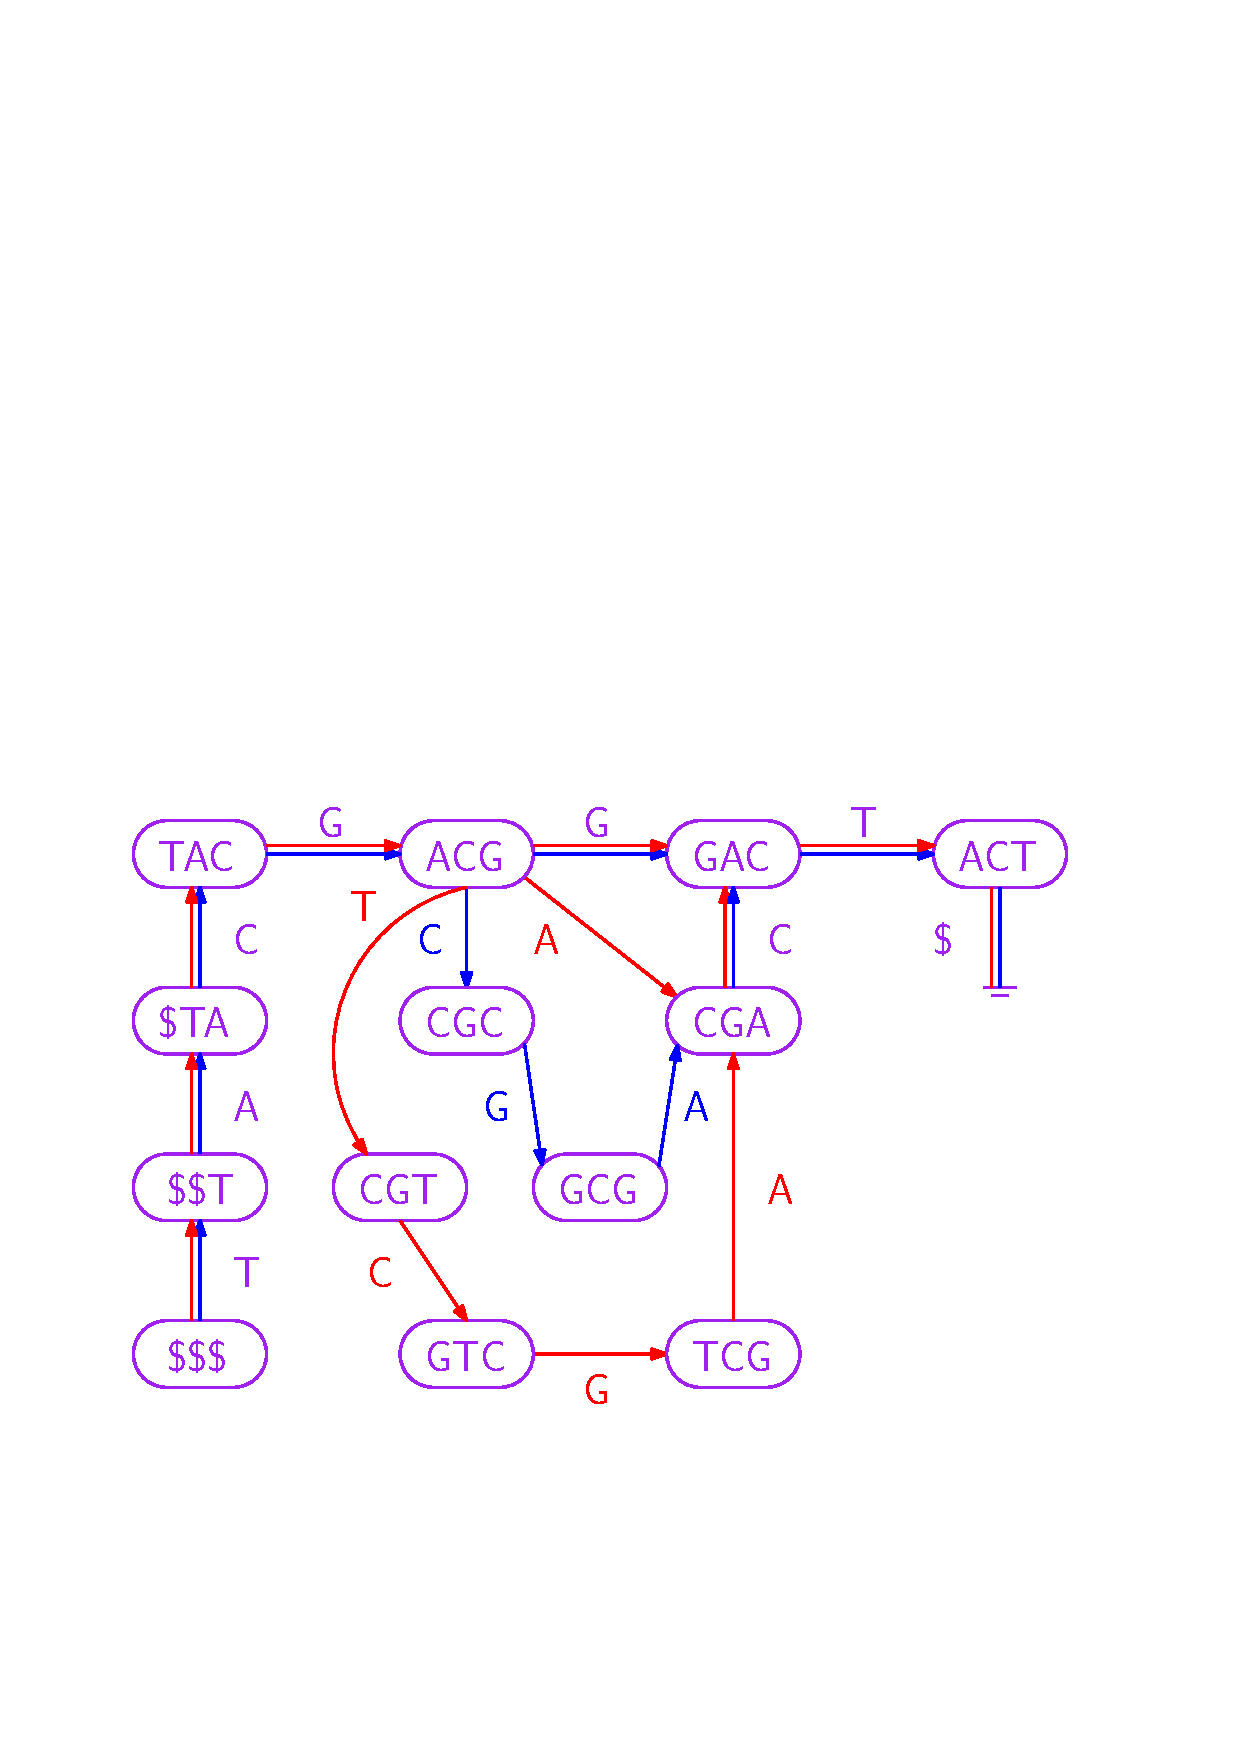
\includegraphics[width=.31\textwidth]{purplegraph} &
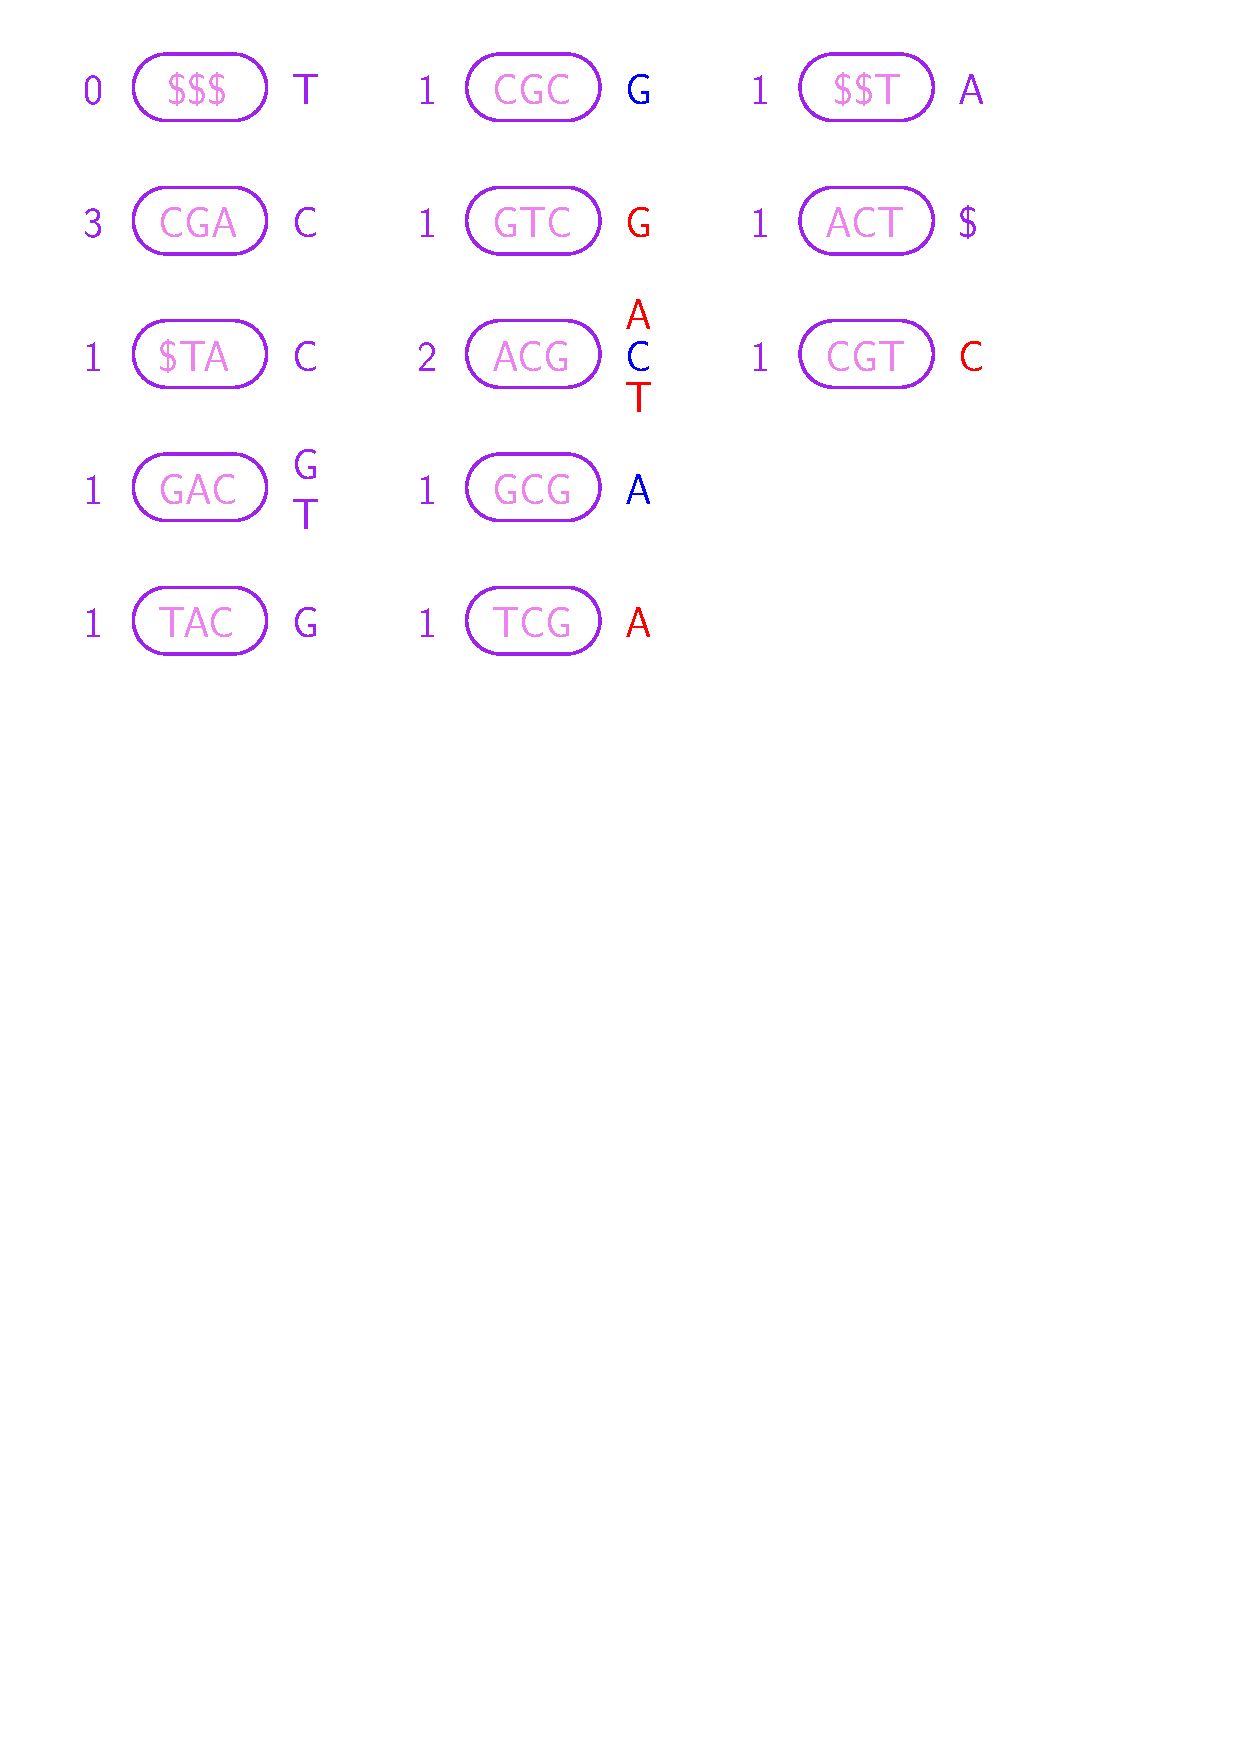
\includegraphics[width=.31\textwidth]{newpurplemapping} &
\raisebox{11ex}{$\begin{array}{rr}
   \EBWT (G) = & \mathtt{TCCGTGGGACTAAA\$C}\\[1ex]
         B_F = & \mathtt{ 001111110111111}\\
         B_L = & \mathtt{1110111100111111}\\[1ex]
C^\mathrm{T} = & \mathtt{0000001001010000}\\
               & \mathtt{0000000110101001}
\end{array}$}
\end{tabular}
\caption{{\bf Left:} A colored de Bruijn graph consisting of two individual graphs, whose edges are shown in red and blue.  (We can consider all nodes to be present in both graphs, so they are shown in purple.)  {\bf Center:} The nodes sorted into co-lexicographic order, with each node's number of incoming edges shown on its left and the labels of its outgoing edges shown on its right.  The edge labels are shown in red or blue if the edges occur only in the respective graph, or purple if they occur in both.  {\bf Right:} Our representation of the colored de Bruijn graph: the edge-BWT and bitvectors for the BOSS representation for the union of the individual graphs, and the binary array $C$ (shown transposed) whose bits indicate which edges are present in which individual graphs.}
\label{fig:purple}
\end{figure*}

\subsection{Implementation}
\label{subsec:implementation}

We now give some details of how our data structure is implemented and constructed in practice.

\subsubsection{Data Structure}

The arsenal of component tools available to succinct data structures designers has grown considerably in recent years~\citep{Navarro16}, with many methods now implemented in libraries. We chose to make heavy use of the succinct data structures library (SDSL)\footnote{\url{https://github.com/simongog/sdsl-lite}} 
in our implementation.

\(\EBWT (G)\), the sequence of edge labels, is encoded in a wavelet tree, which allows us to perform fast rank queries, essential to all our graph navigations. The bitvectors of the wavelet tree  and the $B$ bitvector are stored in the Raman-Raman-Rao (RRR) encoding~\citep{RRR07}.
%[SJP: RRR will be significantly slower than a plain encoding, and I'm not sure it will reduce the size of the WT very much - this is something we need to test. We might even want to use something other than a WT].
The rows of the color matrix, $C$, are concatenated (i.e. $C$ is stored in row-major order) and this single long bit string is then compressed.  It is either stored with RRR encoding,  or alternately Elias-Fano encoding~\citep{elias1974efficient,fano1971number,bitvector} which supports online construction.  Online construction is important for datasets where $C$ is too large to fit in memory in uncompressed form, such as our metagenomic sample dataset.  These encodings reduce the size of $C$ considerably because we expect rows to be very sparse
%(i.e. most $k$-mers are contained in most samples),
and both encodings exploit this sparseness. 
%[SJP: we really should be using the access-optimised encoding that Travis and I suggested --- RRR is overkill and likely slower].

\subsubsection{Construction}

\chapter{Space-efficient CSA construction}\label{chapter:construction}

In this chapter, we investigate the direct construction of compressed suffix arrays, extending the results in Paper~II. We are mostly interested in algorithms whose space usage is dominated by the CSA itself, making it possible to build indexes for texts that are larger than memory size.

The standard way of constructing compressed suffix arrays is to build a suffix array first, and then compress it. There are many existing algorithms \cite{Puglisi2007}, with the best of them working in $O(n)$ time and requiring $2n$ bits of working space in addition to the text and the suffix array \cite{Nong2009}. Yet as a compressed suffix array usually requires less than $n$ bytes of memory \cite{Ferragina2009a}, and can take less than $n$ \emph{bits} with highly repetitive texts (see Section~\ref{sect:rlcsa experiments}), this approach limits the use of CSAs to much smaller texts than could be handled in the available memory.

Many of the suffix array construction algorithms can be adapted to construct the Burrows-Wheeler transform directly. This often replaces the $4n$ to $8n$-byte suffix array with a $n$-byte BWT, reducing memory usage considerably. Yet even the best algorithms \cite{Kaerkkaeinen2007,Okanohara2009} require the text or the BWT --- or both --- in memory, limiting the size of the texts that can be indexed. External memory algorithms for constructing the suffix array \cite{Dementiev2008a} and the Burrows-Wheeler transform \cite{Ferragina2012} exist, but they tend to be slow in practice. In principle, dynamic self-indexes (see Section~\ref{sect:dynamic indexes}) could be used for space-efficient CSA construction, but the implementations seen so far are both slower and require more memory than the alternatives.

Direct algorithms for compressed suffix array construction \cite{Hon2007,Na2007,Hon2009} are the best solution so far. We are especially interested in the algorithm of Hon \etal{Hon2007} that works in $O(n \log n)$ time and requires $\abs{\CSA} + O(n)$ bits of memory. The algorithm essentially uses a static index to simulate CSA construction by a dynamic index, inserting many suffixes in a single update. We describe two practical variants of this algorithm: one that is more space-efficient and another one that can be faster than the original. As the basic building block, we describe an algorithm for merging compressed suffix arrays.

A similar idea has been recently used for constructing the Burrows-Wheeler transform for a large collection of short texts in external memory \cite{Bauer2011}. Instead of inserting large blocks of text at once, the algorithm extends each text by a single character in each step. This way, the algorithm remains simple and has to maintain only a small amount of state information, making it fast and space-efficient in practice. On the other hand, if the texts are longer than a few hundred characters, the algorithm requires too many passes over the data to be useful.


\section{Merging Burrows-Wheeler transforms}\label{sect:merging}

\paragraph{Algorithm of Hon et al.}

The construction algorithm of Hon \etal{Hon2007} can be interpreted as updating the Burrows-Wheeler transform of a text. Assume that we have already constructed $\BWT$ for some text $T$, and we want to update it for $ST$, where $S$ is a sequence of length $l$. We call the suffixes of $ST$ starting in $S$ the \emph{long suffixes} of $ST$, and the rest of the suffixes \emph{short suffixes}.

\begin{definition}
Let $T$ and $T'$ be two texts. The \emph{rank array} $\RA[1,\abs{T'}]$ of text $T'$ relative to text $T$ is an array such that $\RA[i] = \mrank(T, T'[i,\abs{T'}])$. The rank array of a set of suffixes of text $T'$ relative to text $T$ is the corresponding subsequence of array $\RA$.
\end{definition}

The definition also generalizes for collections of texts.

Updating the BWT starts with computing the rank array of long suffixes of text $ST$ relative to text $T$. Backward searching can be used to compute the rank array in a similar way as in the update rule for dynamic compressed suffix arrays (see Section~\ref{sect:dynamic indexes}). A detailed algorithm can be found in Figure~\ref{fig:rank array}.

\begin{figure}
\begin{tabbing}
mm\=mm\=mm\= \kill
\> \textbf{function} $\operatorname{computeRanks}(\mrank(T,T), S, l)$ \\
\> \> $pos \leftarrow \mrank(T, T)$ \\
\> \> \textbf{for} $i \leftarrow l$ \textbf{to} $1$ \\
\> \> \> $pos \leftarrow C[S[i]] + \mrank_{S[i]}(\BWT, pos) + 1$ \\
\> \> \> $\RA[i] \leftarrow pos$ \\
\> \> \textbf{return} $\RA$
\end{tabbing}

\caption{Computing the rank array of long suffixes of text $ST$ relative to text $T$ by backward searching the Burrows-Wheeler transform of $T$.}\label{fig:rank array}
\end{figure}

In addition to determining the lexicographic ranks of long suffixes among short suffixes, we must also determine their ranks among themselves. Conceptually this is done by sorting the long suffixes by their first $l$ characters, breaking ties by using the suffix array of $T$. With both ranks, we can determine the lexicographic ranks of long suffixes among all suffixes.

\begin{lemma}[Fact 1 in \cite{Hon2007}]
The lexicographic rank of a long suffix $S'$ among all suffixes of $ST$ is the sum of its lexicographic ranks among long suffixes and among short suffixes.
\end{lemma}

At this point, we have the lexicographic ranks among long suffixes in suffix array order, and the ranks among short suffixes in text order. By sorting the rank array in increasing order, we get both ranks in suffix array order. This follows from the fact that $S_{1} < S_{2}$ implies $\mrank(T, S_{1}) \le \mrank(T, S_{2})$. Hence the lexicographic ranks of long suffixes among short suffixes must form a non-decreasing sequence, when put into suffix array order. The entire merging algorithm is as follows.

\begin{enumerate}

\item Determine the rank array $\RA$ by the algorithm in Figure~\ref{fig:rank array}. Sort it to get array $\RA'$, and update this array by rule $\RA'[i] \leftarrow \RA'[i] + i$ to get the lexicographic ranks of long suffixes among all suffixes.

\item Sort the long suffixes, and form $\BWT_{S}$ as the subsequence of $\BWT_{ST}$ corresponding to the long suffixes.

\item Update $\BWT_{T}[\mrank(T, T)] \leftarrow S[l]$, and then merge $\BWT_{S}$ and $\BWT_{T}$ to get $\BWT_{ST}$. The merging is done by inserting characters from $\BWT_{S}$ to positions marked in $\RA'$, filling the rest of the positions with characters from $\BWT_{T}$.

\end{enumerate}

\begin{lemma}[Lemma 10 in \cite{Hon2007}]
The above algorithm updates $\BWT_{T}$ to $\BWT_{ST}$ in $O(l \log n + n)$ time, requiring $4l \log n + n + o(n)$ bits of space in addition to $\BWT_{S}$ and $\BWT_{T}$.
\end{lemma}

\paragraph{Merging compressed suffix arrays.}

A simplified version of the above algorithm can be used to merge two compressed suffix arrays. Assume that we have compressed suffix arrays for two texts $T$ and $T'$, and we want to merge them to get a compressed suffix array for the collection $\mathcal{C} = \set{T, T'}$. We select $\CSA_{T}$ as the basic index, and update it to get $\CSA_{\mathcal{C}}$.

In step 1, we get the rank array by searching $\CSA_{T}$ for text $T'$. However, as we are inserting entire texts instead of extending existing texts, we start with $\RA[\abs{T'}] = 1$, as the end marker of $T'$ will come immediately after the end marker of $T$ in lexicographic order. Step 2 is not needed, as we already have $\CSA_{T'}$. Step 3 works as above, except that we are merging compressed BWTs instead of plain BWTs. If we merge the bit vectors of an index of the CSA family one at a time, we are forced to scan the array $\RA'$ at least $\sigma$ times. This can be avoided by merging all bit vectors simultaneously, using a buffer of $\Theta(\sigma)$ characters to avoid polling each of the bit vectors for the next \onebit\ too often.

\begin{lemma}\label{lemma:merging}
The above algorithm merges compressed suffix arrays $\CSA_{T}$ and $\CSA_{T'}$, where $\abs{T'} \le \abs{T}$, in $O(\abs{T'} \cdot (t_{B} + \log \abs{T'}) + \min(\abs{\CSA_{TT'}}, \abs{T}))$ time, where $t_{B}$ is the time required for one step of backward searching. Working space is $\abs{T'} \log \abs{TT'} + O(\sigma \log n)$ bits in addition to the CSAs and $T'$.
\end{lemma}

The lemma applies for indexes of both CSA and FMI families, as long as individual bit vectors can be merged in time relative to their compressed size, and a sequential scan of a bit vector can be done in $O(n_{1})$ time. It generalizes immediately to merging compressed suffix arrays of collections of sequences.

We can also output the rank array directly in suffix array order, avoiding the $O(\abs{T'} \log \abs{T'})$ term in the time bound, if we backward search $\CSA_{T'}$ simultaneously. This allows us to store the array $\RA'$ as a bit vector of length $\abs{TT'}$, which can be much less than the $\abs{T'} \log \abs{TT'}$ bits of a plain array, if the texts are of similar size. We do not even need the text $T'$, as it can be efficiently extracted from $\CSA_{T'}$ (in blocks of $d$ characters in the CSA family, as extraction proceeds in forward direction). In practice, none of these optimizations are very useful, as backward searching is much more expensive than integer sorting.


\section{Construction algorithm}\label{sect:construction}

The merging algorithm can be used as the basic building block of a space-efficient CSA construction algorithm. Assume that we have a large collection of texts $\mathcal{C}$ with total length $N$. The algorithm is as follows, with $\CSA_{i}$ denoting the compressed suffix array of collection $\mathcal{C}_{i}$.
\begin{enumerate}
\item Split the collection into $m$ smaller collections $\mathcal{C}_{1}, \dotsc, \mathcal{C}_{m}$ of size $N/m$.
\item Build $\CSA = \CSA_{1}$, and use it as a basis for the final index.
\item For $i = 2, \dotsc, m$, build $\CSA_{i}$ and merge it with $\CSA$ to get the new $\CSA$.
\end{enumerate}

Note that if there are $r$ sequences in the union of collections $\mathcal{C}_{1}, \dotsc, \mathcal{C}_{i}$, the rank array of collection $\mathcal{C}_{i+1}$ must have value $r$ for each end marker in the collection.

\begin{theorem}
Let $\mathcal{C}$ be a collection of texts with total length $N$ that can be split into $m$ subcollections of size $N/m$. We can use the merging algorithm to construct a compressed suffix array for $\mathcal{C}$ in $O(N + m \cdot \min(\abs{\CSA}, N))$ time using $\abs{\CSA} + \max_{i}(\abs{\CSA_{i}}) + O((N/m + \sigma) \log N)$ bits of space, where $\sigma$ is the size of the alphabet and $\CSA_{i}$ is a CSA for the $i$th subcollection.
\end{theorem}

\begin{proof}
We assume that the CSA is based on bit vectors that support \rank\ and \select\ in $O(1)$ time. By using backward searching on $\CSA_{i}$ to output the rank array directly in suffix array order, we can do all merges within the given time and space bounds. The result follows by using any linear-time suffix array construction algorithm for building the partial indexes $\CSA_{i}$.
\end{proof}

The algorithm can be efficiently parallelized on a single machine. For building the partial indexes, we can either use a parallel suffix array construction algorithm or, if memory allows, index multiple subcollections in parallel. Backward searching can be parallelized, as it does not change the state of the index. Parallel sorting is a well-researched topic, so it does not matter, whether we construct the rank array in text order or in suffix array order. Finally, merging can be parallelized by either merging multiple bit vectors simultaneously, or by dividing a bit vector into multiple parts for merging. If the final CSA is small enough to fit into the memory of a single system, we can also use a computer cluster for construction.


\section{Indexing a single sequence}\label{sect:single sequence}

With practical implementation choices, the algorithm in Section~\ref{sect:construction} uses roughly $(2N/m) \log N$ bits of working space to construct a compressed suffix array for a collection of total size $N$ in $m$ parts, while the algorithm of Hon \etal{Hon2007} uses roughly $(4N/m) \log N + N$ bits. As the algorithms are otherwise almost the same, this represents a significant improvement in space usage without any similar penalty in performance. On the other hand, the collection must be partitioned at sequence boundaries, while the algorithm of Hon et~al.\ can use arbitrary partitioning. In this section, we show how this limitation can be lifted by using $(3N/m) \log N$ bits of working space, with the possibility of making the algorithm faster in practice.

As noted in Section~\ref{sect:merging}, $S_{1} < S_{2}$ implies $\mrank(T, S_{1}) \le \mrank(T, S_{2})$ for any text $T$ and any sequences $S_{1}$ and $S_{2}$. In particular, this means that $T'[i,\abs{T'}] < T'[j,\abs{T'}]$ implies $\RA[i] \le \RA[j]$ in the merging algorithm. Additionally, $T'[i] < T'[j]$ implies $T'[i] + \RA[i] < T'[j] + \RA[j]$. This means that sequence $T' + \RA$ (where $(T'+\RA)[i] = T'[i] + \RA[i]$) has the same suffix array as text $T'$.

\begin{lemma}\label{lemma:rank array}
Let $T$ and $T'$ be two texts. Then $T' + \RA$ has the same suffix array as text $T'$, where $\RA$ is the rank array of text $T'$ relative to text $T$.
\end{lemma}

If text $T$ is much longer than text $T'$, most elements in the rank array are likely to be unique. Hence it should be faster to build a suffix array for the rank array than for the text itself. This gives us the following algorithm.
\begin{enumerate}
\item Split the collection into $m$ smaller collections $\mathcal{C}_{1}, \dotsc, \mathcal{C}_{m}$ of size $N/m$.
\item Build $\CSA = \CSA_{1}$, and use it as a basis for the final index.
\item For $i = 2, \dotsc, m$, determine the rank array $\RA$ of collection $\mathcal{C}_{i}$ relative to the union of all previous collections $\mathcal{C}'$. Build a suffix array of $\mathcal{C}_{i} + \RA$, use it to build $\CSA_{i}$, and merge $\CSA_{i}$ with $\CSA$ to get the new $\CSA$.
\end{enumerate}

We may have to split a text $T = S T'$ into two collections, so that $T' \in \mathcal{C}_{i}$ and $S \in \mathcal{C}_{i+1}$. In this case, we append an end marker to string $S$, and put $x = \mrank(\mathcal{C}',T')$ in the corresponding position in the rank array. As the end marker must be unique to get the correct suffix array, we increment the rank array by $1$ for all other positions $i$, where $\RA[i] \ge x$. Furthermore, if collection $\mathcal{C}'$ contains $r$ texts, and there are $r'$ texts with regular end markers in collection $\mathcal{C}_{i+1}$, we reserve ranks $r, \dots r+r'-1$ for the end markers to get the correct ordering between them, and increment all other values by $r'-1$. Note that we have to remove the position corresponding to the end marker of string $S$ from the suffix array before constructing $\CSA_{i+1}$, as the end marker is not included in the original collection. Note that all changes to the rank array must be reversed, before it can be used in merging.

\begin{theorem}
Let $\mathcal{C}$ be a collection of texts with total length $N$, and let $m > 0$ be an integer. We can use the merging algorithm to construct a compressed suffix array for $\mathcal{C}$ in $O(N + m \cdot \min(\abs{\CSA}, N))$ time using $\abs{\CSA} + \max_{i}(\abs{\CSA_{i}}) + O((N/m + \sigma) \log N)$ bits of space, where $\sigma$ is the size of the alphabet and $\CSA_{i}$ is a CSA for the $i$th subcollection.
\end{theorem}

The working space is now roughly $(3N/m) \log N$ bits, as suffix array construction algorithms generally require $(2N/m) \log N$ bits of writable space with large alphabets, and the rank array must be kept intact during construction.


\section{Implementation}\label{sect:construction implementation}

Two variants of the construction algorithm are included in the implementation of RLCSA (see Chapter~\ref{chapter:rlcsa}). Written in C++, the principal goal of the implementation is to allow indexing text collections that are too large to fit into memory. The implementation has been parallelized by using \emph{OpenMP} and either \emph{MCSTL}\footnote{\url{http://algo2.iti.kit.edu/singler/mcstl/}} or the version of MCSTL integrated into GCC, the \emph{libstdc++ parallel mode}. Both algorithms assume that the collection is stored on disk as a set of $m$ files, each of them less than $4$ gigabytes in size.

First of the algorithms, \emph{Merge}, is an implementation of the algorithm in Section~\ref{sect:construction}. It first builds RLCSAs for all of the subcollections, using a parallelized prefix-doubling algorithm (see below) for the task, and stores them on disk. After all partial indexes have been built, the algorithm starts merging them. Merging has also been parallelized, assuming that the current subcollection consists of multiple texts, so that multiple threads can be used to construct the rank array. The merging phase requires roughly $9n$ bytes of memory in addition to the two RLCSAs, where $n = N/m$ is the size of a subcollection. This includes $8n$ bytes for the rank array and $n$ bytes for the collection. In practice, working space can be significantly more than that, as in-place merging of bit vectors has not been implemented.

The second algorithm, \emph{Fast}, is the algorithm from Section~\ref{sect:single sequence}, except that splitting a text into two subcollections has not been implemented. It processes the subcollections one at a time, using the rank array to build a RLCSA, before merging it with the existing index. This variant uses $25n$ to $29n$ bytes of working space, where the extra $16n$ to $20n$ bytes comes from the suffix array construction algorithm.

Both algorithms use a parallelized \emph{prefix-doubling} algorithm to build the partial indexes. Prefix-doubling-based algorithms are useful for constructing suffix arrays for collections, as we can easily afford having different lexicographic values for the end markers of different sequences. A prefix-doubling algorithm maintains an invariant that array $\SA_{k}$ contains the suffixes in lexicographic order, and array $\RA_{k}$ contains the lexicographic ranks of the suffixes in text order, when the ordering is based on $k$\nobreakdash-character prefixes of each suffix. From these arrays, $\SA_{2k}$ can be determined by sorting $\SA_{k}$ with $(\RA_{k}[\SA_{k}[i]], \RA_{k}[\SA_{k}[i]+k])$ as the sort key for $\SA_{k}[i]$. From $\SA_{2k}$, it is then easy to determine $\RA_{2k}$ in linear time. If sorting is also done in linear time, the prefix-doubling algorithm uses $O(n \log n)$ time for a collection of size $n$.

\newpage The algorithm has been influenced by the suffix array construction algorithm of Larsson and Sadakane \cite{Larsson2007}. If suffix $\SA_{k}[i]$ has already been sorted, we have $\RA_{k}[i] = \RA_{2k}[i]$ and $\SA_{k}[i] = \SA_{2k}[i]$. Hence we have to handle only unsorted ranges in subsequent iterations. To make parallelization easier, we store the unsorted ranges explicitly as pairs of $32$\nobreakdash-bit integers. In the worst case, there can be almost $n/2$ unsorted ranges in both $\SA_{k}$ and $\SA_{2k}$, requiring up to $4n$ bytes of space. In practice, the ranges take at most $n$ bytes of space.

As the first part of the sort key is equal for all suffixes in an unsorted range, we only have to use $\RA_{k}[\SA_{k}[i]+k]$ as the sort key for $\SA_{k}[i]$. To avoid cache misses during sorting, we sort pairs $(\SA_{k}[i], \RA_{k}[\SA_{k}[i]+k])$ of two $32$\nobreakdash-bit integers, instead of retrieving the sort key indirectly. This increases the space usage of the algorithm by $4n$ bytes to a total of $12n$ to $16n$ bytes. Initially, we use the parallel quicksort from MCSTL to sort pairs $(i, T[i,i+1])$ or $(i,T[i])$, depending on whether we can pack two characters into a single $32$\nobreakdash-bit integer. Later, we divide the unsorted ranges between a number of threads, and use the standard sequential sorting algorithm from STL to sort each of the ranges.

The suffix array construction algorithm used in Fast differs from the basic version above. As we are building the suffix array for the rank array instead of the collection, we have to use $64$\nobreakdash-bit sort keys in the initial sorting, and cannot pack two adjacent characters into the key. On the other hand, as the elements of $\RA_{k}$ are $32$\nobreakdash-bit integers, we can pack both $\RA_{k}[\SA_{k}[i]+k]$ and $\RA_{k}[\SA_{k}[i]+2k]$ into the sort key of $\SA_{k}[i]$, and obtain $\SA_{3k}$ instead of $\SA_{2k}$. This prefix-tripling algorithm uses $16n$ to $20n$ bytes of memory, and is usually somewhat faster than the prefix-doubling variant.


\section{Experiments}

To compare the performance of Merge and Fast, we used both algorithms to build RLCSA for two data sets from Paper~II. The first of them, \emph{fiwiki}, is the Finnish language Wikipedia with full version history ($42.03$ gigabytes), while the other, \emph{enwiki}, is a snapshot of the English language Wikipedia ($41.46$ gigabytes). Of the two data sets, fiwiki is a highly repetitive collection. The construction was done on the same system as in Section~\ref{sect:rlcsa experiments}, using 8 parallel threads.

The only other CSA construction algorithm for collections that are too large to fit into memory is the algorithm of Hon \etal{Hon2007} that is essentially an earlier variant of Merge. Some implementations \cite{Lam2008,Li2009} of the algorithm exist, but they can only be used for constructing uncompressed BWT for texts over $2$\nobreakdash-bit alphabets such as DNA sequences. As the algorithms are so similar to each other, any performance differences would most likely be due to implementation choices.

Another way to construct CSAs for collections larger than the main memory is to use an external memory suffix array or BWT construction algorithm. The fastest known general-purpose algorithm is the \emph{bwte} of Ferragina \etal{Ferragina2012}. Distantly related to the algorithm of Hon \etal{Hon2007}, bwte builds an index for the long suffixes, streams the already indexed part of text to determine the \emph{gap array}, and uses the gap array to merge the new index with the existing BWT. The gap array, closely related to the rank array, stores the number of short suffixes falling between two lexicographically adjacent long suffixes. If a collection of size $N$ is indexed in $m$ passes, bwte takes $O(mN)$ time, streams $O(mN \log \sigma)$ bits of data, and requires $O((N/m) \log (N/m))$ bits of working space. As our test environment uses network storage with relatively low transfer rates, it was not reasonable to use it for testing external memory algorithms. Instead, we used a system with a quad-core 2.93 GHz Intel Core i7\nobreakdash-870 processor running OS~X 10.6.8 with bwte. This system had $16$ gigabytes of memory and a solid-state drive.

We split both data sets into $400$\nobreakdash-megabyte subcollections for Merge and Fast, and also used $800$\nobreakdash-megabyte subcollections with Merge. We built RLCSA with default parameters $b = 32$ bytes and $d = 128$. The final index sizes were $14.33$ GB for enwiki and $4.42$ GB for fiwiki. For bwte, we used $1.5$\nobreakdash-gigabyte subcollections, resulting in $28$ (enwiki) and $29$ (fiwiki) passes over the input collection.

In the fiwiki collection, different versions of the same document are stored consecutively. This is almost the worst possible ordering for Fast. If a number of lexicographically adjacent suffixes belong to the same subcollection, they will have the same values in the rank array, and sorting them probably requires many iterations. To test the effect of document ordering, we sorted the sequences in fiwiki by their timestamps. We then compared Merge using $400$ and $800$\nobreakdash-megabyte and $1.5$\nobreakdash-gigabyte subcollections with Fast using $400$\nobreakdash-megabyte subcollections on the new collection \emph{fiwiki-sorted}.

\begin{table}
\centering
\renewcommand{\tabcolsep}{.1cm}
\begin{tabular}{lcccccccccc}
\hline\noalign{\smallskip}
\textbf{Algorithm} & & \textbf{Time} & \textbf{Space} & \textbf{Speed} & & \textbf{Build} & \textbf{Rank} & \textbf{Sort} & \textbf{Merge} & \textbf{I/O} \\

\noalign{\smallskip}
\hline
\noalign{\smallskip}
\multicolumn{10}{l}{\textbf{enwiki}} \\
Merge-400  & & 10.3 & 24.5 & 1.14 & & 3.91 & 1.52 & 0.94 & 3.28 & 0.68 \\
Merge-800  & &  8.6 & 27.0 & 1.36 & & 3.34 & 1.50 & 0.94 & 2.14 & 0.71 \\
Fast-400   & &  8.9 & 30.0 & 1.32 & & 3.24 & 1.51 & 0.92 & 2.97 & 0.28 \\
bwte-1536  & & 84.3 & 12.0 & 0.14 & & --   & --   & --   & --   & --   \\
\noalign{\smallskip}
\multicolumn{10}{l}{\textbf{fiwiki}} \\
Merge-400  & & 11.8 & 11.6 & 1.01 & & 6.96 & 1.38 & 0.87 & 2.23 & 0.37 \\
Merge-800  & & 10.1 & 14.0 & 1.18 & & 5.68 & 1.34 & 0.88 & 1.64 & 0.57 \\
Fast-400   & & 10.5 & 19.4 & 1.14 & & 6.27 & 1.37 & 0.86 & 1.73 & 0.27 \\
bwte-1536  & & 72.9 & 12.0 & 0.16 & & --   & --   & --   & --   & --   \\
\noalign{\smallskip}
\multicolumn{10}{l}{\textbf{fiwiki-sorted}} \\
Merge-400  & & 12.6 & 11.5 & 0.95 & & 7.48 & 1.25 & 0.94 & 2.36 & 0.60 \\
Merge-800  & & 11.2 & 15.0 & 1.07 & & 6.38 & 1.20 & 0.96 & 2.10 & 0.52 \\ 
Merge-1536 & & 11.3 & 22.9 & 1.06 & & 7.08 & 1.18 & 0.95 & 1.66 & 0.45 \\
Fast-400   & & 10.1 & 19.7 & 1.18 & & 5.51 & 1.25 & 0.94 & 2.33 & 0.11 \\
\noalign{\smallskip}
\hline
\end{tabular}

\caption{Indexing two $41$ to $42$\nobreakdash-gigabyte collections. Construction time in hours, memory usage in gigabytes, and construction speed in megabytes per second. For Merge and Fast, the numbers also include a breakdown of time usage between partial index construction (Build), rank array construction (Rank), rank array sorting (Sort), index merging (Merge), and I/O and other overhead (I/O). The number in algorithm name indicates subcollection size in megabytes.}\label{table:construction}
\end{table}

Construction times and memory requirements can be seen in Table~\ref{table:construction}. Note that while the results for bwte include just BWT construction, building RLCSA would not increase construction time significantly. In general, Fast is faster than Merge with the same subcollection size, while Merge offers better time/space trade-offs. However, when the sequences have been sorted by their timestamps, Fast becomes faster than Merge with the same amount of memory, as it can build the partial indexes much faster.
% See Chapter~\ref{chapter:conclusions} for discussion on other ways of using the rank array to speed up partial index construction.

\newpage Both Merge and Fast are much faster than bwte. While bwte is an external memory algorithm, its performance is constrained by CPU speed in practice. Most of the time is taken by the construction of the gap arrays. This requires backward searching for a volume of data equal to roughly $m/2$ times the size of the collection --- more than $500$ gigabytes in these experiments. As backward searching is easy to parallelize, minor modifications should make bwte more competitive on current hardware.

Even though the prefix-doubling algorithm has superlinear time complexity, increasing subcollection size from $400$ megabytes to $800$ megabytes decreases the time required for constructing the partial indexes. A probable explanation is that while the total amount of work increases with block size, the algorithm parallelizes better when sorting larger sets of suffixes. Merging also takes less time with larger block sizes, as fewer merges are required. Still, the effect of subcollection size on running time remains small.

%[SJP: The following overly detailed description is from Alex. To be refined.]
%
%Getting + sorting necessary kmers
%1 read in the node, coverages and edge bitmaps
%2 iterate over the color bitmap, then in an inner loop iterate over
%edge symbols. I then make an inverted symbol by color bit matrix
%3 for each symbol that has a non-zerod row in the matrix, I shift the
%node and append the symbol to make a k-mer (edge)
%4 I reverse the nucleotides of the kmer so it will be sorted in colex
%order, and I also compute the reverse complement
%5 I add (kmer, color-bitmap), (revcomp, color-bitmap) pairs to a
%sorting container (which generates runs, then merges them on access
%later) which drops the last symbol before sorting (table F)
%6 I also add the kmer and revcomp (no color data) to another sorting
%container which sorts based on the whole string (table L)
%Note: In the old version, only 6 was done. The radix sort used two
%tables, so by saving the buffer table we had the second-last iteration
%as well, which meant we had table F
%Note: 5 and 6 are sorted in parallel on different disks for my
%version, so it is faster than a multi-pass version (tested), but also
%uses 2x the disk space. It isnt a radix sort though, so it doesnt
%double the table size. i.e. for both implementations, we use 2x the number 
%of input kmers to add rev comps, then 2x again for F and L.
%
%Generating incoming dummy edges:
%7. i use std::set-difference to take both tables (wrapping the
%iterator so access return just the first k-1 syms from kmers in of F,
%and the last k-1 syms from kmers in L, and both made to be unique - no
%duplicates). This calculates F - L, since any node without a
%predecessor needs an incoming dummy.
%8. it outputs the k-1-mers from F to a provided function, which loops
%(k-2) times to generate \$... \$\$... \$\$\$... (these extra shifts aren't
%technically needed, except to be able to generate the labels for
%incoming dummies again)
%9. each of these is added to another sorter, like above, to be sorted
%on their first k-1 symbols (with \$ sorting before any other symbols).
%Note: before 9, even without all the shifts, the dummies are output in
%the same order as L (colex of whole edge).
%Note: colors dont need to be looked at here (we treat dummies as
%having 0 color for now)
%
%Merging and outgoing dummies:
%Note: You could do a L-F set difference to get outgoing dummies, but
%they are generated in the right order for F, so I combined them into
%one big merge step at the end.
%10. I make a wrapped iterator to access F without the color
%information, but to save it to a color variable that is in scope. This
%way I can merge the color in as I'm writing the kmers out.
%11. I take the two tables F and L, and the dummies. I merge the
%dummies into F (although this time comparing all k symbols), but I
%also calculate the L-F set difference as I'm going. Kind of like a
%3-way merge. If a node is in L that isnt in F, I shift that node and
%append a $ on the right: ....$
%12. each of these is sent to a function, which checks all the first
%k-1 symbols, and last k-1 symbols to generate the B and B' vectors
%(which show the range of entries for nodes in L and F)
%13. the last symbol is written to a file along with the bit vectors
%(interleaved and packed into 64bit blocks)
%14. the color (which is a variable that is now overwritten by the
%iterator wrapper) is written to a separate file.
%
%
%\begin{figure}
%\begin{center}
%\includegraphics[width=.5\textwidth]{New+Doc+5_1.jpg} \\[10ex]
%\caption{Construction of the succinct colored de Bruijn graph, from input to output.}
%\label{fig:construction}
%\end{center}
%\end{figure}

\subsubsection{Traversal}
We implemented two traversal methods based on those of {\sc Cortex} with a modification in light of our intention to apply $\ours$ to metagenomic reads looking for AMR gene presence.

The first, {\it bubble calling}, is a simple algorithm to detect sequence variation in genomic data. It consists of iterating over a set of $k$-mers in order to find places where bubbles start and terminate.  When combined with the $k$-mer color (in a colored de Bruijn graph), this enables identification of places where genomic sequences diverge from one another.  The differing region of the two sequences will form the two arms of a bubble, each colored with only one of the two sequence's colors.  A bubble is identified when a vertex has two outgoing edges. Each edge is followed in turn to navigate a non-branching path until reaching a vertex with two incoming edges. If the terminating vertex is the same for both paths, we call this a bubble. Colors for the bubbles are determined by looking at the color assignment of the corresponding $(k)$-mers. Our implementation in $\ours$ closely follows the pseudocode given by \cite{ICTFM12}.
%; however, it navigates the graph only in a forward direction to see if both paths converge at the same vertex, while {\sc Cortex} navigates the graph backwards and forwards to find a path of adjacent vertices.


{\sc Cortex}'s traversal algorithms were designed for single isolates. For the beef safety experiments, which use metagenomic samples, we implemented a traversal inspired by {\sc Cortex}'s {\it path divergence} algorithm.  In the original {\sc Cortex} path divergence algorithm, bubbles are identified where a user-supplied reference sequence prescribes a walk through a (possibly tangled) sections of the graph in one arm of a bubble while the alternative arm must be branch free.  This branch free requirement on the second arm could be a problem for metagenomic data. Due to the presence of tangle inducing homologous genomes and risk of inferring erroneous, chimeric sequences (which comprise reads from a mix of genomes in the sample), variant detection in metagenomic data is more complex. % FIXME: citation required?
In the absence of a simple metagenomic-aware traversal algorithm, we implemented a variation of the path divergence algorithm which addresses a simpler problem, primarily for the purpose of measuring performance.  This algorithm uses a reference guided approach and allows us to measure the memory footprint at traversal time as well as the time savings of not traversing the entire dataset.  For this purpose, we focus specifically on the presence of AMR genes (our reference sequence) rather than variants of those genes; in our derived algorithm we ignore sample path segments leading away from and returning to the AMR gene path.  This avoids some of the problems with tangles, incomplete coverage, or read errors.  Thus as we traverse the gene path, we simply count the number of samples in each sample group that color the current edge.   We note that keeping $C$ in row major order allows us to compute this count in constant time as the difference between two $\rank$ queries.  







%% \subsubsection{{\sc\bf Cortex}'s Graph Implementation}

%% Before discussing our experimental results, we give a brief description of the colored de Bruijn graph data structure that is implemented in the current {\sc Cortex} release, which we use as a baseline to measure our performance against in the next section. 

%% {\sc Cortex} implements the colored de Bruijn graph using a hash table. Each entry in the hash table stores a $(k - 1)$-mer (vertex in the graph) as well as the following fields: the $(k-1)$-mer labelling this vertex, {\sf coverage} (an array, indexed by color), {\sf status}, and {\sf edges} (indicating adjacent $(k - 1)$-mers in the graph). 

%% The $(k-1)$-mer part of the hashtable entry is a compile time determined length, composed of multiple 64-bit fields (sufficient to accommodate $k-1$ nucleotides, represented as two bits each).
%% The coverage information is used for error correction prior to graph construction, e.g., to remove low-coverage $k$-mers assumed to be the result of sequence errors. Later, when processing the graph, the {\sf coverage} array is used to determine if a $k$-mer exists for a given color (coverage of 0 for a given color indicates the $(k-1)$-mer does not exist in that sample). The {\sf status} field is used at runtime to record whether the vertex has been previously visited, and to store other information specific to a given algorithm (e.g. bubble finding). Finally, an {\sf edges} field is stored for each $k$-mer and each color. It is one byte in size, and each of the eight bits indicate which bases precede and follow the $k$-mer for this color. Since there are four possible predecessors and successors, one byte is sufficient.

\section{Results} \label{sec:results} 

\subsection{Datasets} \label{subsec:data}

Our first dataset consists of approximately 6.9 million paired-end 101 bp reads from the prokaryote genome {\em Francisella tularensis}, generated by Illumina Genome Analayzer (GA) IIx platform. 
It was obtained from the NCBI Short Read Archive (accession number SRR063416). The reference genome was also downloaded from the NCBI website (Reference genome NC\_006570.2).  
The {\em  Francisella tularensis} genome is 1,892,775 bp in length. As a measure of quality assurance, we aligned the reads to the {\em Francisella tularensis} genome using BWA (version 0.5.9) \cite{bwa} with default parameters.  
We call a read {\em mapped} if BWA outputs an alignment for it and {\em unmapped} otherwise.  
Analysis of the alignments revealed that 97\% of the reads mapped to the reference genome, representing an average depth of approximately $367\times$.  

Our second dataset consists of approximately  31.3 million paired-end 100 bp reads from the loblolly pine  ({\em Pinus taeda} L.) genome~\cite{pine}.  
We downloaded the reference genome from the pine genome website~\cite{pinetreeweb} and simulated reads from the largest five hundred scaffolds from the reference using ART~\cite{art} (art illumina). 
% FIXME: What does the read simulator do with runs of N's in scaffolds?  How do these affect our pipelines?
ART was ran with parameters that simulated 100 bp paired end reads with 200 bp insert size and 50x coverage.  
The substitution error rate was reduced to one 10th of the default profile.  
The data for this experiment is available on the $\sequel$ website.  
We simulated an optical map using the reference genome for {\em Francisella tularensis} and loblolly pine since there is no publicly available one for these genomes.  


%Our second dataset consists of approximately 6.9 million paired-end 100 bp reads from the prokaryote genome {\em Porphyromonas gingivalisi}, generated by Illumina Genome Analayzer (GA) IIx platform. It was obtained from the NCBI Short Read Archive (accession number SRR413299). The reference genome was also downloaded from the NCBI website (Reference genome NC\_002950.2).  The {\em  Porphyromonas gingivalisi} genome is 2,343,476 bp in length. As a measure of quality assurance, we aligned the reads to the reference genome using BWA (version 0.5.9) with default parameters~\cite{bwa}.   This analysis of the alignments revealed that 98\% of the reads mapped to the reference genome, representing an average depth of approximately $404\times$.  


\begin{table}[h!]
\begin{center}
\caption{The performance comparison between major assembly tools on the \emph{Francisella tularensis} dataset  (1,892,775 bp, 6,907,220 reads, 101 bp)  using QUAST in default mode \cite{quast}. 
All statistics are based on contigs no shorter than 500 bp. N50 is defined as the length for which the collection of all contigs of that length or longer contains at least half of the sum of the lengths of all contigs, and for which the collection of all contigs of that length or shorter also contains at least half of the sum of the lengths of all contigs.  
\# unaligned is the number of contigs that did not align to the reference genome, or only partially aligned (part).  
Total is sum of the length of all contigs. 
MA is the number of (extensively) misassembled contigs.  
local MA is the total number of contigs that had local misassemblies. 
MA (bp) is the total length of the MA contigs.  
GF is the genome fraction percentage, which is the fraction of genome bases that are covered by the assembly. 
--rr and ++rr denotes before and after repeat resolution, respectively.}
\begin{tabular}{|c|c|c|c|c|c|c|c|c|c}
\hline
\textbf{Assembler} 			&{\bf \# contigs }		& \textbf{N50}	& \textbf{Largest (bp)}	& \textbf{Total (bp) }	&\textbf{MA}	&\textbf{local MA}	& {\bf MA (bp)} 		& \textbf{GF (\%)} \\ 
 						&{\bf (\# unaligned) }		& 			& 					& 				&			& 			& 				& \\ \hline
Velvet					& 358 (3 + 35 part)		& 7,377		& 39,381				& 1,762,202 		& 11			& 36			& 84,965			& 92.09			  \\ \hline
SOAPdenovo 				& 307 (3 + 31 part)		& 8,767		& 39,989				& 2,018,158 		& 10			& 35			& 96,258			& 92.05				\\ \hline
ABySS					& 96 (1 part)  			& 27,975  		& 88,275				& 1,875,628		& 64  		& 32			& 1,330,684		& 95.87  			 	 \\ \hline
SPAdes (--rr)				& 102 (2 + 11 part) 		&  25,148		& 87,449				& 1,788,634		& 11 			& 30			& 258,309			& 92.81			 	 \\ \hline
SPAdes (+rr)				& 100 (2 + 17 part) 		&  26,876		& 87,891				& 1,797,197 		& 23 			& 31			& 497,356			& 93.75			 	 \\ \hline
IDBA						& 109 (1 + 10 part)		& 23,223 		& 87,437 				& 1,768,958		& 10			& 31			& 221,087			& 92.64  				 \\ \hline
%HyDA					& 					&			&  					&  				&  			&			&				& 			 	 \\ \hline
\end{tabular}
\label{tab:ging}
%\end{center}
%\end{table}
%\begin{table}[ht!]
%\begin{center}
\vspace{10mm}
\caption{\footnotesize{The performance comparison between major assembly tools on Loblolly pine ({\em Pinus taeda} L.) genome dataset (62,647,324 bp, 31.3 million reads, 100 bp) using QUAST in default mode \cite{quast}.}}
\label{tab:pine}
\begin{tabular}{|c|c|c|c|c|c|c|c|c|c}
\hline
\textbf{Assembler} 			&{\bf \# contigs }		& \textbf{N50}	& \textbf{Largest (bp)}	& \textbf{Total (bp) }	&\textbf{MA}	&\textbf{local MA}	& {\bf MA (bp)} 		& \textbf{GF (\%)} \\ 
 						&{\bf (\# unaligned) }		& 			& 					& 				&			& 			& 				& \\ \hline
Velvet					& 13,327 (0)			& 1,740		& 10,823				& 51,851,131 		& 0			& 0			& 0				& 62.21			  \\ \hline
SOAPdenovo 				& 16,126 (0 + 1 part)		& 7,950		& 63,004				& 57,205,817 		& 0			& 0			& 0				& 90.01				\\ \hline
ABySS					& 4,586 (16 + 89 part)  	& 37,089  		& 201,382				& 63,349,408		& 127  		& 715		& 1,391,565		& 98.17  			 	 \\ \hline
SPAdes (--rr)				& 20,671 (4 + 10 part) 	& 4,809		& 44,993				& 45,079,764		& 7 			& 11			& 65,079			& 81.30			 	 \\ \hline
SPAdes (+rr)				& 8,607 (7 + 102 part) 	& 16,957		& 108,442				& 59,730,939 		& 299 		& 57			& 3,734,609		& 94.57			 	 \\ \hline
IDBA						& 22,409 (3 + 31 part)	& 3,990 		& 40,213				& 49,765,854		& 61			& 200		& 292,769			& 79.03  				 \\ \hline
\end{tabular}
\end{center}
\end{table}


We assembled both sets of reads with a wide variety of state-of-the-art assemblers.  The versions used were those that were publicly available before or on September 1, 2014: 
%These were: 
SPAdes (version 3.1)~\cite{spades}; Velvet (version  1.2.10)~\cite{Zerbino:2008}; SOAPdenovo (version 2.04)~\cite{soap}; ABySS (version 1.5.2)~\cite{Simpson:2009}; and IDBA-UD (version 1.1.1)~\cite{idbaud}.
SPAdes outputs two assemblies: before repeat resolution and after repeat resolution --- we report both.
Some of the assemblers emitted both contigs and scaffolds.  We considered contigs only but note that all scaffolds had a greater number of misassembly errors. 
{\em We emphasize that our purpose here is not to compare the various assemblers, but demonstrate that all assemblers produce misassembly errors, which are in need of consideration and correction.  } 

We used Quast \cite{quast} in default mode to evaluate the assemblies.  
Quast defines misassembly error as being {\em extensive} or {\em local}.  
A (extensive) misassembled contig is defined as one that satisfies one following conditions:  (a) the left flanking sequence aligns over 1 kbp away from the right flanking sequence on the reference; (b) flanking sequences overlap on more than 1 kbp; (c) flanking sequences align to different strands or different chromosomes. 
Whereas, a local misassembled contig is one that satisfies the following conditions: (a) two or more distinct alignments cover the breakpoint; (b) the gap between left and right flanking sequences is less than 1 kbp; and the left and right flanking sequences both are on the same strand of the same chromosome of the reference genome.  
We made a minor alteration to Quast to output which contigs contain local misassembly errors.  
A contig can contain both extensive and local misassembly errors.  
Any correctly assembled contig is one that does not contain either type of error.  

\subsection{Detection of Misassembly Errors in {\em Francisella tularensis}} \label{sec:tularensis}

Table~\ref{tab:ging} gives the assembly statistics corresponding to this experiment.  
Comparable assembly results on this data were reported by Ilie et al.~\cite{sage}, though in some cases we used more recent software releases (e.g., for SPAdes).  
Note that the number of locally misassembled contigs and the number of extensively misassembled contigs is not disjoint.
A contig can be locally and extensively misassembled.   
Thus, Table \ref{tab:ging} gives the number of contigs having at least one extensive misassembly error, and the number of contigs having at least one local misassembly error.

\begin{table}[h!]
\begin{center}
\caption{The performance comparison of our method on the \emph{Francisella tularensis} dataset. 
The true positive rate (TPR) in this context is a contig that is misassembled and is predicted to be so. 
The false positive rate (FPR) is a correctly assembled contig that was predicted to be misassembled.
The TPR and FPR is given as a percentage with the raw values given in brackets}
{\setlength{\tabcolsep}{1em}
\begin{tabular}{|l|c|c|c|c|}
\hline
\textbf{Correction Method}								& \textbf{Assembler}		&{\bf MA TPR}			& {\bf local MA TPR}		& \textbf{FPR}	\\ \hline
							& Velvet				& 100\% (11 / 11)		& 100\% (36 / 36)		& 58\% (180 / 312)		\\ 
							& SOAPdenovo		& 100\% (10 / 10)		& 100\% (35 / 35)		& 63\% (165 / 263)	\\ 
 misSEQuel								& ABySS				& 100\% (64 / 64)		& 100\% (32 / 32)		& 87\% (20 / 23)			\\ 
(paired-end data only)				& SPAdes (--rr)			& 100\% (11 / 11)		& 100\% (30 / 30)		& 83\% (52 / 63)		\\ 
							& SPAdes (++rr)		& 100\% (23 / 23)		& 100\% (31 / 31)		& 86\% (49 / 57)		\\ 
							& IDBA				& 100\% (10 / 10)		& 100\% (31 / 31)		& 38\% (57 / 149) \\ \hline \hline
				
							& Velvet				& 55\% (6 / 11)			& 69\% (25 / 36)			& 24\% (76 / 312)	\\ 
							& SOAPdenovo		& 80\% (8 / 10)			& 63\% (22 / 35)			& 29\% (77 / 263)	\\ 
misSEQuel					& ABySS				& 69\% (44 / 64)		& 88\% (28 / 32)			& 13\% (3 / 23)		\\ 
(optical mapping data only)		& SPAdes (--rr)			& 91\% (10 / 11)		& 87\% (26 / 30)			& 21\% (13 / 63)		\\ 
							& SPAdes (++rr)		& 87\% (20 / 23)		& 81\% (25 / 31)			& 16\% (9 / 57)			\\ 
							& IDBA				& 90\% (9 / 10)			& 77\% (24 / 31)			& 10\% (15 / 149)		\\ 
\hline \hline
					
							& {\bf Velvet}					& {\bf 55\% (6 / 11)}			& {\bf 100\% (26 / 36)}		&	{\bf 22\% (68 / 312)}	\\ 
							& {\bf  SOAPdenovo}				& {\bf 80\% (8 / 10)}			&{\bf 84\% (21 / 35)}			&	{\bf 20\% (53 / 263)}	\\
 {\sc\bf misSEQuel}				& {\bf ABySS}					& {\bf 69\% (44 / 64)}			& {\bf 88\% (28 / 32)}			&	{\bf 13\% (3 / 23)}		\\ 
{\bf (paired-end and optical}	& {\bf  SPAdes (--rr)}				&{\bf 91\% (10 / 11)}			& {\bf 87\% (26 / 30)}			&	{\bf 19\% (12 / 63)}		\\ 
{\bf mapping data)}				& {\bf SPAdes (++rr)}				&{\bf 97\% (20 / 23)}			& {\bf 81\% (25 / 31)}			&	{\bf 16\% (9 / 57)}		\\ 
							& {\bf IDBA}					&{\bf 90\% (9 / 10)}			&{\bf  77\% (24 / 31)}			&	{\bf 9\% (14 / 149)}		\\ 
\hline \hline
							& Velvet						& 55\% (6 / 11)		& 11\% (4 / 36)				& $<$ 1\% (2 / 312)		\\ 
							& SOAPdenovo				& 20\% (2 / 10)		& 14\% (5 / 35)				& 2\% (6 / 263)	\\  
REAPR						& ABySS						& 13\% (8 / 64)		& 13\% (4 / 32)				& 4\% (1 / 23)			\\  
							& SPAdes (--rr)					& 27\% (3 / 11)		& 27\% (8 / 30)				& 5\% (3 / 63)			\\ 
							& SPAdes (++rr)				& 0\% (0 / 23)		& 19\% (6 / 31)				& 11\% (6 / 57)		\\
							& IDBA						& 40\% (4 / 10)		& 13\% (4 / 31)				& 4\% (6 / 149)			\\ 
\hline
\end{tabular}}
\label{tab:roc}
\end{center}
\end{table}



Table \ref{tab:roc} shows the results for: (a) $\sequel$ with paired-end data only; (b) $\sequel$ with optical mapping data only; and (c) $\sequel$ with both optical mapping and paired-end data in order to demonstrate the gain of combining both types of data.  
As demonstrated by these results, using short read paired-end data alone produces a high false positive rate, since it is unable to distinguish between structural variations within the genome and misassembly errors.  
This is an inherent shortcoming of short read data and demonstrates that in order to decrease the false positive rate, another source of information must be used in combination.
Optical mapping data has a much lower false positive rate and when used in combination with paired-end data, produces optimal results.  The lowest false positive rate was witnessed when both optical mapping and paired-end data were used.  In some cases, the reduction in the false positive rate was dramatic; from 87\% (ABySS, paired-end data) to 13\% (ABySS, paired-end and optical mapping data).  The true positive rate of locally misassembled contigs was between 77\% and 100\% when both paired-end and optical mapping data were used.  Lastly, true positive rate of extensively misassembled contigs was between 55\% and 100\% when both paired-end and optical mapping data were used. 

In our experiments, we iterate through combinations of three enzymes from the REBASE enzyme database \cite{roberts2010rebase} and use the set of enzymes that performed best.  
Our results demonstrate that with a good enzyme choice over half of all extensively misassembled contigs, and over 75\% of locally misassembled contigs can be identified with only a 9\%-22\% false discovery rate.
 
\subsection{Detection of Misassembly Errors in Loblolly Pine}\label{sec:pine}

The results for the loblolly pine are shown in Table \ref{tab:roc_pine}.  Both Velvet and SOAPdenovo produced zero misassembled contigs on this dataset, so we do not include them in Table~\ref{tab:roc_pine}.
% just shows results for the remaining assemblies.
$\sequel$ correctly identifies between 31\% and 100\% of extensively misassembled contigs, and between 57\% and 73\% of locally misassembled contigs.  The false positive rate was between 0.6\% and 43\%.  Although, REAPR has a lower false positive rate (between 3\% and 11\%), it is only capable of identifying a small number of extensively misassembled contigs (between 2\% and 14\%) and a small number of locally misassembled contigs (between 2\% and 27\%).  

Lastly, the restriction enzymes used in our experiments were chosen to be optimal by considering the set of all possible enzymes in the aformentioned database.  
Nonetheless, we note that if the enzyme combination was chosen at random then the expected false positive rate and true positive rate would decrease by a small fraction for majority of the assemblies considered.  
See the Appendix for prototypical ROC curves and heatmaps illustrating the density of enzyme combinations at various detection rates.



\begin{table}[h!]
\begin{center}
\caption{The performance comparison of our method on the loblolly pine dataset. 
Again, a true positive in this context is a contig that is misassembled and is predicted to be so. 
A false positive is a correctly assembled contig that was predicted to be misassembled.}
{\setlength{\tabcolsep}{1em}
\begin{tabular}{|l|c|c|c|c|}
\hline
\textbf{Correction Method}& \textbf{Assembler} 		&{\bf MA TPR}				& {\bf local MA TPR}					& \textbf{FPR}	 \\ \hline
 					& {\bf ABySS}				&  {\bf 31\% (40 / 127)}		&  {\bf 57\% (405 / 715)} 		  	 	& {\bf 43\% (1,604 / 3,754)}		 	 \\ 
{\sc\bf misSEQuel}		& {\bf SPAdes (--rr)}			&  {\bf 100\% (7 / 7)}			&  {\bf 73\% (8 / 11)}			 		& {\bf $<$1\% (135 / 20,653)	}	 	 \\ 
					& {\bf SPAdes (+rr)}			&  {\bf 67\% (199 / 299)}		& {\bf 67\% (38 / 57)}			 		& {\bf 38\% (3,117 / 8,254)} 		 	 \\ 
					& {\bf IDBA}				&  {\bf 52\% (32 / 61)}		&  {\bf 73\% (145 / 200)} 		  	 	& {\bf 19\% (4,258 / 22,150)}			 \\ 
\hline 
					& ABySS					& 7\% (9 / 127) 				& 2\% (12 / 715) 		  			& 3\% (112 / 3,754)		 \\  
 REAPR				& SPAdes (--rr)				& 14\% (1 / 7)				& 27\% (3 / 11)		 				& 6\% (1,323 / 20,653)		 	 \\ 
					& SPAdes (+rr)				& 7\% (21 / 299)			& 5\% (3 / 57)		 				& 5\% (424 / 8,254)	 \\ 
					& IDBA					& 2\% (1 / 61)				& 6\% (12 / 200)		  	 		&11\% (2,354 / 22,150)		 \\  
\hline
\end{tabular}}
\label{tab:roc_pine}
\end{center}
\end{table}


\subsection{Practical Considerations: Memory and Time} \label{mem_time}

We evaluated the memory and time requirements of $\sequel$.   Since $\sequel$ is a multi-threaded application, its wall-clock-time depends on the computing resources available to the user.  
$\sequel$ required a maximum of 8 threads, 16 GB and 1.5 hours on all assemblies of {\em  Francisella tularensis}, and a maximum of 20 GB and 2.5 hours to complete on all assemblies of loblolly pine.
Most genome assemblers require an incomparably greater amount of time and memory and thus, from a practical perspective, the requirements of $\sequel$ are not a significant increase.  
The difference in the resource requirements of $\sequel$ in comparison to modern assemblers is due to the fact it operates contig-wise rather than genome-wise and therefore, only deals with a significantly smaller portion of the data at a single time.
We conclude by mentioning that $\sequel$ is not optimized for memory and time and both could be further reduced but reimplementing the red-black positional de Bruijn graph using memory and time succinct data structures. 


\chapter{Conclusions}
\label{sec:conclusions}

%\section{Future Work}
%\label{sec:future-work}


%\subsection*{Acknowledgements}
%The authors would like to thank Journi Sir\'{e}n from the Wellcome Trust Sanger Institute for many insightful discussions, and Zamin Iqbal for his assistance with testing {\sc Cortex}.




%
%\section{Experiments}
\label{sec:experiments}

\begin{table}[t!]
%\caption{Construction Time and Memory Usage (top), and Mean Time per Navigation Operation (lower).}
\caption{Input size (top), construction time, memory use, and structure size (middle), and mean time taken for each 
navigation operation (lower), for all data sets and both structures. For variable-order, the multipliers in
parenthesis are the increase over the fixed-order results. Cells marked ``N/A'' for fixed-order indicate operations not
possible with that structure.
%The times in parentheses for $\longer$ are the mean times per node in the resulting set.
}
\scriptsize
\setlength\tabcolsep{1.8pt}
\begin{tabularx}{\textwidth}{@{}Rd{3.2}d{4.9}d{3.2}d{4.9}d{3.2}d{5.9}d{3.2}d{5.9}@{}}
% manual : http://ftp.jaist.ac.jp/pub/CTAN/macros/latex/required/tools/tabularx.pdf
						%\cline{2-9}
\toprule
{\bf Dataset}     & \multicolumn{2}{c}{{\em E.~coli}} & \multicolumn{2}{c}{Human chromosome 14} & \multicolumn{2}{c}{Human} 		& \multicolumn{2}{c}{Parrot} \\
% I think DSK size + number of K-mers is enough to demonstrate the increasing data set size
% I don't have times for DSK, so I'd have to run those again if needed
%Genome Size (bp) & \multicolumn{2}{c}{{4,639,221}} & \multicolumn{2}{c}{88,289,540} & \multicolumn{2}{c}{} 		& \multicolumn{2}{c}{} \\
%Number of Reads & \multicolumn{2}{c}{{}} & \multicolumn{2}{c}{} & \multicolumn{2}{c}{} 		& \multicolumn{2}{c}{} \\
%\midrule
%K & \multicolumn{2}{c}{{27}} & \multicolumn{2}{c}{55} & \multicolumn{2}{c}{55} 		& \multicolumn{2}{c}{55} \\
%Frequency Threshold & \multicolumn{2}{c}{{1}} & \multicolumn{2}{c}{1} & \multicolumn{2}{c}{2} 		& \multicolumn{2}{c}{1} \\
%DSK Time (mins) & \multicolumn{2}{c}{{}} & \multicolumn{2}{c}{} & \multicolumn{2}{c}{} 		& \multicolumn{2}{c}{} \\
{\bf DSK Size (GB)} & \multicolumn{2}{c}{{1.52}} & \multicolumn{2}{c}{6.88} & \multicolumn{2}{c}{26.74} 		& \multicolumn{2}{c}{70.28} \\
{\bf\boldmath Number of $K$-mers} & \multicolumn{2}{c}{{204,098,902}} & \multicolumn{2}{c}{461,445,333} & \multicolumn{2}{c}{1,794,522,954} 		& \multicolumn{2}{c}{4,716,731,435} \\
{\bf BOSS Order} & \multicolumn{1}{c}{fixed} 	& \multicolumn{1}{c}{variable} & \multicolumn{1}{c}{fixed} 	& \multicolumn{1}{c}{variable} & \multicolumn{1}{c}{fixed} 	& \multicolumn{1}{c}{variable} & \multicolumn{1}{c}{fixed} 	& \multicolumn{1}{c}{variable} \\
\midrule
%\cline{1-9}
{\bf Construction (mins)} & 3.93 & 5.09 \enspace (1.30{\sf x}) & 14.37 & 18.72 \enspace (1.30{\sf x}) & 64.45 & 83.85 \enspace (1.30{\sf x})& 162.58 & 225.73 \enspace (1.39{\sf x})\\
{\bf Graph Size (GB)}  			   & 0.16  & 0.41 \enspace (2.56{\sf x})  & 0.40   & 1.38 \enspace (3.45{\sf x}) & 1.67 & 5.42 \enspace (3.25{\sf x}) & 4.20 & 13.60 \enspace (3.24{\sf x}) \\
{\bf Peak RAM (GB)}  		 & 3.16 & 3.16 \enspace (1.00{\sf x}) & 3.22 & 3.22 \enspace (1.00{\sf x})& 7.65 & 9.31 \enspace (1.22{\sf x}) & 15.30 & 15.29 \enspace (1.00{\sf x}) \\
{\bf Peak Disk (GB)}  	 & 12.17 & 12.17 \enspace (1.00{\sf x}) & 56.68 & 56.68 \enspace (1.00{\sf x}) & 248.37 & 248.37 \enspace (1.00{\sf x}) & 562.28 & 562.28 \enspace (1.00{\sf x})\\
%\cline{1-9}
\midrule
$\forward$ ($\mu$s)   & 6.00 & 17.03 \enspace (2.84{\sf x}) &6.24	&16.17 \enspace (2.59{\sf x}) &7.07	&18.31 \enspace (2.59{\sf x})&7.77	 &19.39 \enspace (2.50{\sf x})\\
$\backward$ ($\mu$s)  & 8.23 & 59.77 \enspace (7.26{\sf x}) &8.47	&55.63 \enspace (6.57{\sf x}) &9.27	&62.85 \enspace (6.78{\sf x})&10.46 &63.87 \enspace (6.11{\sf x})\\
$\lastchar$ ($\mu$s)  & 0.01 &  0.01 \enspace (1.00{\sf x}) &0.01	& 0.01 \enspace (1.00{\sf x}) &0.01	& 0.01 \enspace (1.00{\sf x})&0.01	 &0.01 \enspace (1.00{\sf x})\\

$\maxlen$ ($\mu$s)    &\multicolumn{1}{r}{N/A}  & 1.43   &\multicolumn{1}{r}{N/A} &1.56	   &\multicolumn{1}{r}{N/A}  	&2.02	    &\multicolumn{1}{r}{N/A}  &2.46 \\ 
$\maxlen_c$ ($\mu$s)  &\multicolumn{1}{r}{N/A}  &	5.41  &\multicolumn{1}{r}{N/A} &5.98	   &\multicolumn{1}{r}{N/A}  &6.71	    &\multicolumn{1}{r}{N/A}  &7.49 \\
$\shorter_1$ ($\mu$s) &\multicolumn{1}{r}{N/A}   &	14.65 &\multicolumn{1}{r}{N/A} &17.72	 &\multicolumn{1}{r}{N/A} 	  &19.54	  &\multicolumn{1}{r}{N/A}  &19.84 \\
$\shorter_2$ ($\mu$s) &\multicolumn{1}{r}{N/A}  &	14.83 &\multicolumn{1}{r}{N/A} &17.79	 &\multicolumn{1}{r}{N/A}  	&19.68	  &\multicolumn{1}{r}{N/A}  &19.98 \\
$\shorter_4$ ($\mu$s) &\multicolumn{1}{r}{N/A}   &	15.11 &\multicolumn{1}{r}{N/A} &18.02	 &\multicolumn{1}{r}{N/A}   &19.90	  &\multicolumn{1}{r}{N/A}  &20.20 \\
$\shorter_8$ ($\mu$s) &\multicolumn{1}{r}{N/A}   &	15.73 &\multicolumn{1}{r}{N/A} &18.39	 &\multicolumn{1}{r}{N/A}   &20.29	  &\multicolumn{1}{r}{N/A}  &20.64 \\
%$\shorter$ ($\mu$s)   &\multicolumn{1}{r}{N/A}   &	15.08 &\multicolumn{1}{r}{N/A} &17.98	 &\multicolumn{1}{r}{N/A}   &19.85	  &\multicolumn{1}{r}{N/A}  &20.17 \\ % mean avg of above 4
$\longer_1$ ($\mu$s)  &\multicolumn{1}{r}{N/A}   &21.53   &\multicolumn{1}{r}{N/A} &18.61	 &\multicolumn{1}{r}{N/A}   &21.06	  &\multicolumn{1}{r}{N/A}  &20.57 \\ 
$\longer_2$ ($\mu$s)  &\multicolumn{1}{r}{N/A}  &56.96   &\multicolumn{1}{r}{N/A} &41.08	 &\multicolumn{1}{r}{N/A}   &49.01	  &\multicolumn{1}{r}{N/A}  &47.07\\
$\longer_4$ ($\mu$s)  &\multicolumn{1}{r}{N/A}   &503.60  &\multicolumn{1}{r}{N/A} &323.50	 &\multicolumn{1}{r}{N/A}   &446.51	  &\multicolumn{1}{r}{N/A}  &428.97 \\
$\longer_8$ ($\mu$s)  &\multicolumn{1}{r}{N/A}  &6441.33 &\multicolumn{1}{r}{N/A}  &5338.38 &\multicolumn{1}{r}{N/A}   &18349.80	&\multicolumn{1}{r}{N/A}  &24844.80 \\

%$\longer_1$ ($\mu$s)  &\multicolumn{1}{r}{N/A} &21.53 \enspace (10.82)  &\multicolumn{1}{r}{N/A} &18.61 \enspace (12.38)  &\multicolumn{1}{r}{N/A} &21.06 \enspace (13.25)    &\multicolumn{1}{r}{N/A} &20.57 \enspace (12.99)\\ 
%$\longer_2$ ($\mu$s)  &\multicolumn{1}{r}{N/A} &56.96 \enspace (8.74)   &\multicolumn{1}{r}{N/A} &41.08 \enspace (11.24)  &\multicolumn{1}{r}{N/A} &49.01 \enspace (11.74)    &\multicolumn{1}{r}{N/A} &47.07 \enspace (11.02)\\
%$\longer_4$ ($\mu$s)  &\multicolumn{1}{r}{N/A} &503.60 \enspace (7.98)  &\multicolumn{1}{r}{N/A} &323.50 \enspace (10.59) &\multicolumn{1}{r}{N/A} &446.51 \enspace (11.04)   &\multicolumn{1}{r}{N/A} &428.97 \enspace (9.95)\\
%$\longer_8$ ($\mu$s)  &\multicolumn{1}{r}{N/A} &6441.33 \enspace (6.44) &\multicolumn{1}{r}{N/A} &5338.38 \enspace (9.03) &\multicolumn{1}{r}{N/A} &18349.80 \enspace (10.09) &\multicolumn{1}{r}{N/A} &24844.80 \enspace (9.48)\\

%$\longer_1$ nodes&	N/A	39.80	N/A	30.06	N/A	31.78	N/A	31.66
%$\longer_2$ nodes&	N/A	130.32	N/A	73.11	N/A	83.48	N/A	85.42
%$\longer_4$ nodes&	N/A	1262.84	N/A	610.77	N/A	809.06	N/A	861.91
%$\longer_8$ nodes&	N/A	20010.15	N/A	11824.04	N/A	36370.68	N/A	52388.38
\bottomrule
%\cline{2-9}
\end{tabularx}
% $\dagger$ $\lastchar$ is a reverse lookup in a very small array, so the speed is in fractions of a nanosecond.
% $\ddagger$ $\longer$ is reported as the average time  for the inputs $1$,$2$,$4$,$8$, due to much longer calculation time. }
\label{tab:nav-time}
\end{table}

%We have implemented the faster version of our data structure on top of an efficient implementation of the BOSS single-$K$ data structure\footnote{The
We have implemented the wavelet tree based data structure on top of an efficient implementation of the BOSS single-$K$ data structure\footnote{The
implementation is released under GPLv3 license at \url{http://github.com/cosmo-team/cosmo}. As Cosmo is under continuous development,
a static snapshot of the code used in this paper is available at \url{https://github.com/cosmo-team/cosmo/tree/varord-paper}.}.
Both structures make use of the SDSL-lite software library\footnote{\url{https://github.com/simongog/sdsl-lite}} for succinct data structures, and the
the construction code makes use of the STXXL software library\footnote{\url{https://github.com/stxxl/stxxl}} for external memory data structures and sorting.
The construction code is also concurrent in many places.%, making use of C++11 threads, and OpenMP\footnote{\url{http://openmp.org/}} for parallel internal memory sorting.
The smaller but slower version was not implemented.
%Further implementation details are described in \ref{sec:implementation}.

% TODO : cite their algorithmic paper?
% What makes STXXL good:
% http://stxxl.sourceforge.net/tags/master/introduction.html
% http://stxxl.sourceforge.net/tags/master/design.html
% http://stxxl.sourceforge.net/tags/master/design_algo_sorting.html
% http://stxxl.sourceforge.net/tags/master/citelist.html

% System
Our test machine was a server with a hyperthreaded quad-core 2.93 Ghz Intel Core i7-875K CPU and 16 GB RAM running
Ubuntu Server 14.04. Four Samsung 850 EVO 250GB SSDs were used for temporary storage for STXXL,
with a fifth identical drive used for temporary storage for SDSL-Lite and final graph output. In order to make
use of STXXL's parallel disk and asynchronous I/O support\footnote{\url{http://stxxl.sourceforge.net/tags/master/design_algo_sorting.html}},
the SSDs were not in a RAID configuration. The input files were read from a mechanical 2TB 7200 RPM disk.
% I might have been able to load the DSK files from a SSD thinking back... but it wouldn't make a difference except faster run time *for everything*

To minimize the effect of external factors on our results, each experiment was repeated three times with the minimum values
reported. The swap file was disabled, forcing the operating system to keep each graph completely in memory, and
there were no other users on the server.

% TODO : should construction be moved up and merged with the above?
% TODO : describe the construction algorithm
% TODO : describe why we needed external construction

\subsection{Test Data}

%To assess assembly quality, we aligned the reads to the {\em E.~coli} reference genome (substr.  K-12) using BWA (version 0.5.9) \cite{li2009fast} with default parameters.  We call a read {\em mapped} if BWA outputs an alignment for it and {\em unmapped} otherwise.  Analysis of the alignments revealed that 98\% of the reads mapped to the reference genome, representing an average depth of approximately $600\times$.  Next, we determined the amount of memory and time needed for our method for a larger dataset.  For that, we 
%The reference genome was also downloaded from the website (Reference genome GCA\_000001405.16).  
% Analysis of the alignments revealed that 98\% of the reads mapped to the reference genome, which represents 
% approximately 47x coverage of the genome.

In order to test the scalability of our approach, we repeated the experiment on readsets of varying size.
Our first data set consists of 27 million paired-end 100 character reads (strings)
from {\em E.~coli} (substr.  K-12). It was obtained from the NCBI Short Read Archive (accession 
ERA000206, EMBL-EBI Sequence Read Archive). The total size of this data set is around 2.3 GB compressed on disk (6 GB uncompressed).

The second data set is 36 million 155 character reads from the Human chromosome 14 Illumina reads used in the GAGE
benchmark\footnote{\url{http://gage.cbcb.umd.edu/}}, totalling 1.3 GB compressed on disk (6 GB uncompressed).

For our third data set we obtained 1,415 million  paired-end 100 character Human genome reads
(SRX01231) that were generated by Illumina Genome Analyzer (GA) IIx platform. The total size of this data set is 130 GB compressed on disk (470 GB uncompressed).

Our fourth data set is 700 million paired-end 101 character reads, and 131 paired-end 75 character reads from the short
insert libraries of the Parrot data (ERA201590) provided in Assemblathon 2\cite{assemblathon2}.
The total size of this data set is 64 GB compressed on disk (245 GB uncompressed).

%We ran DSK on each... The human data set required too much external memory, and the final dBG size would have been too large to fit in internal memory,
%so had to be re-run with the frequency threshold set to 2.

We used DSK~\cite{dsk} on each data set to find the unique $(K+1)$-mers.
It is usual to have DSK ignore low-frequency $(K+1)$-mers (as they may result from sequencing errors). 
However, removing such $(K+1)$-mers may result in the removal of some $k$-mers with $k \leq K$ that would 
otherwise have an acceptable frequency. We therefore set the frequency threshold to be as low as possible: $1$ (accepting 
all $(K+1)$-mers) for all data sets except for the Human genome data set, which was too big for our SSDs during construction,
and too big to fit into RAM afterwards. Hence, for the Human genome data set, the frequency threshold was $2$.

%\footnote{This increases the resulting size, but the size relative to the standard BOSS representation can still be compared.
%Variable-$K$ frequency filtering can be implemented using the $L^*$ vector, but will affect the dummy edge calculations, and
%is hence designated as future work.}.
% TODO: mention mercy kmers (Megahit) as another strategy? ultimately we just don't want gaps

A value of $K = 27$ was chosen
%\footnote{Note that the BOSS de Bruijn graph is defined in terms of $K+1$-mers, so DSK must be run for $K+1$ (i.e. 28 and 56) rather than for $K$.}
for the {\em E.~coli} data, and $K = 55$
for the Human data sets as these values produced good assemblies in previous papers (see, e.g.,~\cite{paul}). $K = 55$ was also chosen for the Parrot
data set, %as there was no clear choice for $K$ from the Assemblathon 2 contestants, and
as it produced a graph that almost filled the main memory.
The resulting file sizes and $(K+1)$-mer totals are shown in Table~\ref{tab:nav-time}.

% TODO: Run experiment with one data set over multiple Ks to see how it scales that way

% TODO: Time DSK (multithreaded) (I don't have timings for these)
%DSK took 28 and 58 minutes to run on the {\em E.~coli} and human data sets, respectively.

\subsection{Construction}
\label{sec:construction}

In order to convert the input DSK data to the format required by BOSS (in the correct order, with dummy edges, as required by both single-$K$ and variable-$K$ structures),
we use the following process, which has been designed with disk I/O in mind.

While reading the DSK input data, we generate and add the reverse complements for each $(K+1)$-mer, then sort them by their first $K$ symbols (the source nodes). Concurrently, we also sort another copy of the $(K+1)$-mers and their reverse complements by their last $K$ symbols (the target nodes). Let the resulting tables
be $A$ and $B$, respectively.

Next, we calculate the set differences $A-B$, comparing only the $K$-length prefixes to the $K$-length suffixes respectively. This tells us which source nodes do not
appear as target nodes, which we prepend with $\$$ signs to create the required incoming dummy edges ($K$ each), and then sort by the first $K$ symbols. Concurrently, we also calculate $B-A$ to give us
the nodes requiring outgoing dummy edges (to which we append $\$$). Let the resulting tables be $I$ and $O$, respectively. At this point $B$ can be deleted.
%\footnote{This will create duplicate strings, which can be avoided using Longest Common Prefix calculations.}.

Finally, we perform a three-way merge (by first $K$ symbols) of $A$, $I$, and $O$, outputting the rightmost column. In the case of the variable-$K$ graph,
we also calculate the $L^{*}$ values while merging. Finally, we construct the necessary succinct indexes from the output.

The time bottleneck in the above process is clearly in sorting the $A$ and $I$ tables. $|I|$ can be as big as $K|A|$, but in practice only $1\%$ or fewer
nodes require incoming dummies. Our elements are of size $\Oh{K}$, thus, overall, construction of both data structures takes $\Oh{K^2|A|\log|A|}$ time
and $\Oh{K^2|A|}$ space in theory, but in practice takes $\Oh{K|A|\log|A|}$ time and $\Oh{K|A|}$ space.

%The large file sizes necessitated an external construction scheme.

% Draw attention to the limited difference
%The only place that construction differs for the variable order de Bruijn graph is during the merge, where the longest common suffix length is calculated
%for consecutive edges, and written to disk. Finally, when constructing the rank and select structures, the variable order de Bruijn graph creates a Wavelet Tree
%as well.


\subsection{Results}

For each data set, the $(K+1)$-mers from DSK (and their reverse complements) were converted into the BOSS format
using the process outlined in \ref{sec:construction}, using the external memory vectors and multithreaded, external
memory sort from STXXL. The BOSS structure and $L^{*}$ wavelet tree were then built using indexes from SDSL-lite.

Construction times and structure sizes are shown in Table~\ref{tab:nav-time}.
While the variable-$K$ BOSS structure is around $30\%$ slower to build, and $2.6$ to $3.5$ times larger 
than the standard BOSS structure, this is clearly much faster and less space consuming than building 
$K$ separate instances of the BOSS structure. The peak RAM and disk usage is the same for both structures
except in the case of the Human genome data set, where the variable-$K$ BOSS structure used $22\%$ more RAM.
% TODO : repeat, if same results, trace RAM usage, work out why?

% identical peak disk and RAM
% TODO : Does this sounds week since we didn't measure building/storing each static-k dbg individually?
% TODO : Should we compare it to megahit?

%% TODO: fix the xs in this table? \times doesnt handle \em well though
%\begin{table}[h!]
%\begin{tabularx}{\textwidth}{@{\extracolsep{\fill} } r  c  c   c  c }
%						& \multicolumn{2}{c}{{\em Escherichia coli}} 		& \multicolumn{2}{c}{Human chromosome 14} \\
%						\cline{2-5}
%   						& BOSS 		& multi-K BOSS			& BOSS  		&  multi-K BOSS  \\
%\hline
%Wall Time (mins) & 19  & 25 {\em(1.32x)} & 153 & 203 {\em(1.33x)} \\
%Final Size (MB)  & 163 & 420 {\em(2.58x)} & 414 & 1416 {\em(3.42x)}\\
%Genome Size (bp) 	&  \multicolumn{2}{c}{4,639,221} 			&  \multicolumn{2}{c}{88,289,540} \\
%Number of Reads 			&  \multicolumn{2}{c}{27 M} 				&  \multicolumn{2}{c}{36.5 M}  \\
%DSK Time (mins) 	&  \multicolumn{2}{c}{28} 			&  \multicolumn{2}{c}{58} \\
%\hline
%\end{tabularx}
%\caption{Summary of data sets, as well as construction time and final space for BOSS de Bruijn graph and multi-$K$ de Bruijn graph. For the multi-$K$ BOSS representation, the
%increase factor is shown in parentheses.}
%\label{tab:build}
%\end{table}

%Due to the non-trivial engineering effort required to integrate a particular de Bruijn graph 
%structure in a live assembler, we compare our new data structure to the original BOSS structure
%by measuring average times for navigation operations.
To measure navigation functions $\forward$ and $\backward$ we took the mean time 
over 20,000 random queries. For the variable-$K$ graph, the $k$ values for each node 
were chosen randomly between $8$ and $K$. 
%(involves only a reverse lookup on a very small array). 
Results are shown in Table~\ref{tab:nav-time}. 
The new structure makes the $\forward$ operation $2.5$ to $3$ times slower for $k < K$, though we 
note that for $k = K$ $\forward$ time is identical.
The $\backward$ operation is much slower in the new structure, but is much less frequently 
used than $\forward$ in assembly algorithms (for a variation that supports fast
$\backward$ calculations, see \cite{varorder-latin}). We also measured $\lastchar$, which took only
nanoseconds on both structures.

To see how fast the order can be changed, we timed $\shorter$ and $\longer$ for
changes of $1$, $2$, $4$, and $8$ symbols. Our experiments show that in practice changing 
order by a single symbol ($\shorter_1$ and $\longer_1$) is a cheap operation, taking around the
same time as $\forward$. For larger changes in order, the time for $\shorter$ is stable
($\shorter_1$, $\shorter_2$, $\shorter_4$, and $\shorter_8$ all take roughly the same time),
whereas $\longer$ takes significantly more time as the difference in order increases. This is because
$\longer$ must compute a set of nodes, and the size of that set grows roughly exponentially with
the change in order ($\longer$ takes around $10 \mu$s per node when averaged over the size of the resulting set).
%If not every node in the result is to be visited, the set could instead be calculated lazily.

As expected, $\maxlen$ is very fast (it requires a single rank and select operation
over a bit vector), and only slightly affected when finding the specified outgoing edge label (which
uses a rank and select over the BOSS wavelet tree instead).

% TODO: add separate measurements for 2,4,8... but as order changes increase, the... factor is more evident.



%
%\chapter{Conclusions}
\label{sec:conclusions}

%\section{Future Work}
%\label{sec:future-work}

%
%\chapter*{Acknowledgements}

First and foremost, I could not have completed my PhD without the sponsorship of Soukendai and NICTA.

I’d also like to thank the following people for mentoring me:

\begin{itemize}
\item \textbf{Justin Zobel} -- You helped me secure funding to start my PhD, and introduced me to the de Bruijn graph and DNA assembly. Without your help, I may not have started a PhD. You also taught many of the professors I had in University, so I owe a lot to you transitively speaking, too.
\item \textbf{Kathryn Holt} -- Thank you for spending countless hours teaching me about biology in your office. Coming from a school that taught creationism, this was mind expanding, and incredibly influential on the way I would think in general.
\item \textbf{Tom Conway} -- You kicked off the succinct de Bruijn graph subfield, and took the time to help me understand your paper over several lunches.
\item \textbf{Simon Puglisi} -- Thank you for introducing me to succinct data structures. I think I’ve always done my best work whenever I’m with you, whether that is writing a paper, or rolling a cigarette and having a glass of wine in Helsinki.
\item \textbf{Kunihiko Sadakane} -- Thank you for helping a young student pursue his dream of doing a PhD in succinct data structures in Japan, and being patient when I spent too much time having fun in Tokyo. You have encyclopedic knowledge, and I was incredibly lucky to be your student.
\item \textbf{Uno Takeaki} -- You were always able to calm my anxieties of being a 30-something PhD student, and encouraged me to enjoy writing my dissertation. Thank you for your guidance, patience, and understanding.
\item \textbf{Martin Muggli} -- Thank you for being somebody I could ask questions that I really should already know the answer to, and for carrying the codebase on. Thanks as well for the real-talk. I learned a lot about myself from you.
\item \textbf{Travis Gagie, Jouni Siren, and Christina Boucher} -- co-authors, incredibly smart and creative, and a pleasure to work with.
\item \textbf{James Harland} -- For introducing me to research, encouraging exploration, and for being a fantastic mentor.
\item \textbf{Rayan Chikhi, Dinghua Li, Sean Jackman, Jared Simpson, Roberto Grossi, Rajeev Raman, and Srinivasa Rao Satti} -- For being available to answer my questions about a field that was new to me, and for making me feel like a welcome member of our research community.
\item \textbf{Nick Greenfield and Nava Whiteford} -- For hiring me as a succinct de Bruijn graph consultant!
\item \textbf{James Hayton and Javier Grande} -- This dissertation has been a monkey on my back for years, but you cut through my anxieties and helped me get it done.
\end{itemize}

Of my family and friends, these people helped me immeasurably:

\begin{itemize}
\item \textbf{John Bowe} -- For finding out exactly how cheap Tokyo is not. Thanks for sponsoring me.
\item \textbf{Christine Mulvey -- Thank you for helping me learn to program as a kid -- I remember you debugging my basic programs that I typed in from library books. And for doing my assignments in school} -- why didn’t you do my dissertation though!?
\item \textbf{James and Nikolas Bowe} -- For the brotherly encouragement and competition. I can finally say I’m better than you both.
\item \textbf{Christian Sea Jones} -- Thanks for looking after me in Tokyo, as well as laughing every time I said “I’m trying to finish my dissertation”. Do or do not, there is no try.
\item \textbf{Ellen Chou} -- For being the first person I met in Tokyo, showing me the cool bars and how to do purikura, and giving me an amazing birthday present a few days after I moved there.
\end{itemize}

It was incredibly nostalgic to sit here and write this list and reflect on how grateful I am to have met each of you.


%\appendix
%\include{chapters/tables}

% Enable this to list all bibliography entries
%\nocite{*}

\bibliographystyle{unsrt}
\bibliography{bibliography}

\end{document}
